\documentclass{UVKABoA4}

\usepackage{graphicx} % Standardpaket zur Grafikeinbindung
\usepackage{amsmath,amssymb} % Erweiterung des Mathematik-Modus
\usepackage[colorinlistoftodos, german]{todonotes} % Option 'disable' entfernt alle ToDos
\usepackage[absolute,overlay]{textpos}
\usepackage{vmargin}          % Adjust margins in a simple way
\usepackage{tikz}
\usepackage{subcaption}
\usepackage{textcomp}

\usepackage{algorithm}
\usepackage{algpseudocode} 

% Toggle the following two lines to switch between english and german layout
\usepackage[english]{babel} % Neue deutsche Rechtschreibung und Silbentrennung.


\usepackage[raiselinks=true,
            bookmarks=true,
            bookmarksopenlevel=1,
            bookmarksopen=true,
            bookmarksnumbered=true,
            hyperindex=true,
            plainpages=false,
            pdfpagelabels=true,
            pdfborder={0 0 0.5}]{hyperref}


\makeatletter

\def\tagform@#1{\maketag@@@{\ignorespaces [#1]\unskip\@@italiccorr}}	% Anpassung der Formelnummerierung
\makeatother

\makeindex

\newcommand{\myname}{Forename~Surname}
\newcommand{\headtitle}{Title of thesis\\ 
                        Second title line}
\newcommand{\floatingtitle}{Title of thesis - Second title line}
\newcommand{\thesistype}{Master thesis}

\newcommand{\reviewerone}{Prof.~Dr.--Ing.~J.~M.~Zöllner}
\newcommand{\reviewertwo}{Prof.~Dr.--Ing.~R.~Dillmann}
\newcommand{\advisor}{Dipl.--Inform.~Max~Mustermann}

\newcommand{\timestart}{XX. Monat 20XX}
\newcommand{\releaseyear}{2016}
\newcommand{\timeend}{XX. Monat \releaseyear}
\newcommand{\releasemonth}{in Monat \releaseyear}


% Names of the organizations
\newcommand{\department}{\iflanguage{english}{Department of Computer Science}
                                             {Fakultät für Informatik}}
\newcommand{\institute}{\iflanguage{english}{Institute for Anthropomatics}
                                            {Institut für Anthropomatik}}
\newcommand{\fzidepartment}{Abteilung Technisch Kognitive Assistenzsysteme}
\newcommand{\fziname}{\iflanguage{english}{FZI Research Center for Information Technology}
                                          {FZI Forschungszentrum Informatik}}

% A graphic best describing your thesis
\newcommand{\titlefig}{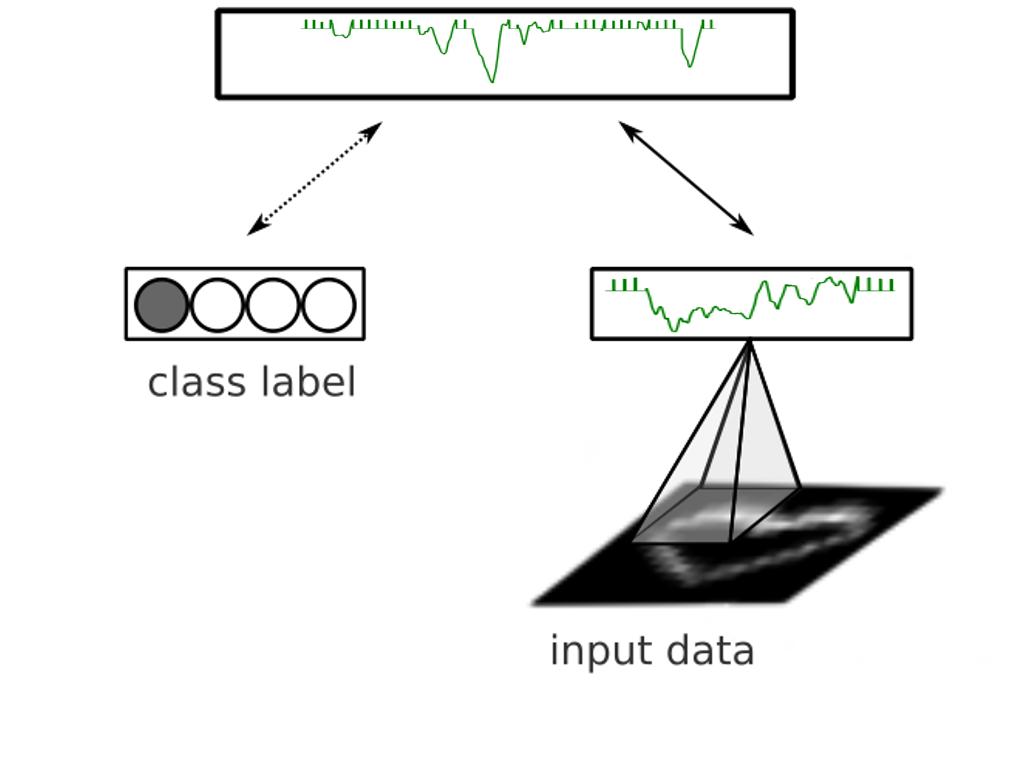
\includegraphics[width=1.0\textwidth]{graphics/not-the-final-title}}

\begin{document}

\pagenumbering{roman}
%% titlepage.tex
%%

% coordinates for the bg shape on the titlepage
\newcommand{\diameter}{20}
\newcommand{\xone}{-25}
\newcommand{\xtwo}{150}
\newcommand{\yone}{25}
\newcommand{\ytwo}{-243}

\begin{titlepage}
% bg shape
\begin{tikzpicture}[overlay]
\draw[color=gray]  
 		 (\xone mm, \yone mm)
  -- (\xtwo mm, \yone mm)
 arc (90:0:\diameter pt) 
  -- (\xtwo mm + \diameter pt , \ytwo mm) 
	-- (\xone mm + \diameter pt , \ytwo mm)
 arc (270:180:\diameter pt)
	-- (\xone mm, \yone mm);
\end{tikzpicture}
  \begin{textblock}{10}[0,0](3.35,2.55)
	  \iflanguage{english}  {
\includegraphics[width=.3\textwidth]{graphics/kitlogo_en_rgb}}
                          {
\includegraphics[width=.3\textwidth]{graphics/kitlogo_de_rgb}}
  \end{textblock}
	\changefont{phv}{m}{n}	% helvetica	
	\vspace*{2.5cm}
	\begin{center}
		\Huge{\headtitle}
		\vspace*{2cm}\\
		\Large{
			\iflanguage{english}{Master Thesis of}			
												  {Masterarbeit\\von}
		}\\
		\vspace*{1cm}
		\huge{\myname}\\
		\vspace*{1cm}
		\Large{
			\department\\ \institute\\ \iflanguage{english}{and}{und}\\ \fziname
		}
	\end{center}
	\vspace*{1.5cm}
\Large{
\begin{center}
\begin{tabular}[ht]{l c l}
  \iflanguage{english}{Reviewer}{Erstgutachter}: & \hfill  & \reviewerone\\
  \iflanguage{english}{Second reviewer}{Zweitgutachter}: & \hfill  & \reviewertwo\\
  \iflanguage{english}{Advisor}{Betreuender Mitarbeiter}: & \hfill  & \advisor\\
  % \iflanguage{english}{Second advisor}{Zweiter betreuender Mitarbeiter}: & \hfill  & \advisortwo\\
\end{tabular}
\end{center}
}


\vspace{2cm}
\begin{center}
\large{\iflanguage{english}{Research Period}{Bearbeitungszeit}: \timestart \hspace*{0.25cm} -- \hspace*{0.25cm} \timeend}
\end{center}


\begin{textblock}{10}[0,0](4,16.8)
\tiny{ 
	\iflanguage{english}
		{KIT -- University of the State of Baden-Wuerttemberg and National Research Center of the Helmholtz Association}
		{KIT -- Universität des Landes Baden-Württemberg und nationales Forschungszentrum in der Helmholtz-Gemeinschaft}
}
\end{textblock}

\begin{textblock}{10}[0,0](14,16.75)
\large{
	\textbf{www.kit.edu} 
}
\end{textblock}

\end{titlepage}

\pagestyle{empty}
\begingroup
\changefont{phv}{m}{n}
\renewcommand{\baselinestretch}{1}

\begin{titlepage}
  \parindent 0em 
  \LARGE\textbf{\floatingtitle}
  \vspace{24pt}\\
  \iflanguage{english}{by}{von}\\
  \myname \\[1.5cm]
  \begin{center}
  \titlefig\\[1cm]
  \end{center}
  \vfill
  \begin{minipage}{0.4\textwidth}
    \begin{flushleft} \large
      \LARGE\textbf{\thesistype}\\
      \LARGE\releasemonth
    \end{flushleft}
  \end{minipage}
  \begin{minipage}{0.6\textwidth}
    \begin{flushright}
      
\includegraphics[width=1.5cm]{graphics/FZI-Logo}
    \end{flushright}
  \end{minipage}
  \newpage
  \small \thesistype, FZI\\
  \department, \releaseyear\\
  Gutachter: \reviewerone, \reviewertwo
  \vfill
  \fzidepartment\\
  \fziname
  \newpage
\end{titlepage}

\endgroup

% \thispagestyle{empty}

\begin{center}
  \vspace*{\stretch{1}}
  \bfseries
  \LARGE
  \headtitle\\[0.45cm]
  \vfill
  \mdseries
  \huge
  \thesistype\\[0.8cm]
  \large
  Abteilung Technisch Kognitive Assistenzsysteme\\[0.1cm]
  Forschungszentrum Informatik\\[0.1cm]
  an der\\[0.1cm]
  Universität Karlsruhe (TH)\\
  \vfill
  von\\[0.3cm]
  \LARGE
  \myname\\
  \vfill
  \normalsize
  \begin{tabular}{p{3.5cm} p{0.4cm} p{5.5cm}}
    \textbf{Tag der Ausgabe} & : &  \timestart\\
    \textbf{Tag der Abgabe}  & : &  \closingdate\\
    & & \\
    & & \\
    & & \\
    \textbf{Betreuer} & : & \advisor \\
    \textbf{Referent} & : & Prof.~Dr.--Ing.~J.~M.~Zöllner \\
    \textbf{Koreferent} & : & Prof.~Dr.--Ing.~R.~Dillmann
  \end{tabular}
\end{center}

\parindent 1em
\affirmation

Ich versichere wahrheitsgemäß, die Arbeit selbstständig angefertigt, alle benutzten Hilfsmittel vollständig und genau angegeben und alles kenntlich gemacht zu haben, was aus Arbeiten anderer unverändert oder mit Abänderungen entnommen wurde.

\vspace{2cm}
\begin{flushright}\noindent
    Karlsruhe,\hfill {\it \myname}\\
    \releasemonth \hfill { }
\end{flushright}
% \preface

Diese \LaTeX{}-Vorlage, basierend auf \emph{KOMA}-Script-Klasse\index{KOMA-Script} scrbook\index{scrbook}, wurde erstellt, um Veröffentlichungen im Universitätsverlag\index{Universitätsverlag} Karlsruhe in einem einheitlichen Layout zu ermöglichen. Die Dokumentklasse\index{Dokumentklasse} \emph{UVKABook}\index{UVKABook} soll dabei unverändert bleiben. Sollten zusätzliche Pakete geladen werden, muss sichergestellt sein, dass keine Veränderungen am bestehenden Layout erfolgen. Der Inhalt des Manuskripts wird im Unterordner \emph{content} abgelegt und in das Hauptdokument \emph{book.tex} eingebunden. Bestehende Abschnitte etwa für das Vorwort\index{Vorwort} oder die Danksagung\index{Danksagung} können einkommentiert werden. Unter Umständen kann es notwendig sein, dass einzelne Pakete nachinstalliert werden (beispielweise das \emph{KOMA-Script} oder \emph{natbib}\index{natbib}). Das Literaturverzeichnis\index{Literaturverzeichnis} verwendet \emph{bibtex}. Bei Rückfragen wenden Sie sich bitte an den Universitätsverlag Karlsruhe.

\vspace{1cm}
\begin{flushright}\noindent
    Karlsruhe,\hfill {\it \myname}\\
    \releasemonth \hfill { }
\end{flushright}
% 
\abstract

Extracting high level features in data automatically can benefit various tasks such as classification and prediction. 
Deep belief networks allow to build feature extractors in an unsupervised manner. 
Utilizing a convolutional multilayered architecture can further improve the quality of the features on compositional data and allow a more abstract representation. 
Most architectures perform operations in discrete time steps and do not utilize a continuous information processing similar to the brain, which could lead to faster response times and a lower power consumption. 
In this thesis we propose different biologically inspired architectures to build and train a spiking deep belief network with a convolutional architecture. 
Two different training algorithms are presented.
The first approach trains the network in discrete time steps and the resulting network is afterwards transformed into a spiking neural network.
The second approach trains a spiking network directly with an adapted spike time dependent plasticity learning rule and weight synchronization.
Both algorithms are evaluated on different discrete and event-based datasets.
On the different datasets the algorithms are able to discriminate classes with high accuracy without any modification of the learning rules, thus indicating an adaptive feature extraction algorithm.
By comparing both approaches it becomes apparent that by introducing lateral inhibitory connections the directly trained algorithm is able to extract more discriminative features.
 
\chapter*{Zusammenfassung}

Die automatische Extraktion von "High-Level Features" unterstützt und erleichtert Aufgaben wie Klassifikation und Prädiktion.
Mit Hilfe von Deep Belief Networks können solche Feature Extraktoren unüberwacht gelernt werden.
Durch eine vielschichtige Convolutional Architektur kann die Feature Qualität auf kompositionellen Daten weiter verbessert werden und eine abstraktere Repräsentation ermöglicht werden.
Die meisten Architekturen arbeiten, im Gegensatz zum Gehirn, in diskreten Zeitschritten und nutzen keine kontinuierliche Informationsverarbeitung, was zu schnel-leren Verarbeitungszeiten und einer niedrigeren Leistungsaufnahme führen könnte.
In dieser Arbeit werden verschiedene biologisch motivierte Architekturen vorgestellt, die es ermöglichen ein Convolutional Spiking Deep Belief Network aufzubauen und zu trainieren.
Es werden zwei verschiedene Ansätze präsentiert.
Der erste Ansatz trainiert ein Netzwerk in diskreten Zeitschritten und wandelt danach das trainierte Netzwerk in ein Spiking Netzwerk um.
Der zweite Ansatz trainiert direkt ein Spiking Netzwerk mit einer angepassten Version der "Spike-Time dependent plasticity" Lern-Regel mit Parameter-Synchronization.
Die Ansätze werden auf verschiedenen diskreten und Event-basierten Datensätzen evaluiert.
Beide Ansätze erreichen auf den verschiedenen Datensätzen eine hohe Klassifikationsgenauigkeit ohne die zugrunde liegenden Lern-Regel zu verändern, was auf einen adaptionsfähig Feature-Extraktions Algorithmus schließen lässt.
Der Vergleich der beiden Ansätze legt nahe, dass aufgrund von lateral-hemmenden Verbindungen der zweite Ansatz diskriminativere Features extrahieren kann. 

        
% 
\ack

Die vorliegende Arbeit entstand während meiner Tätigkeit als wissenschaftlicher Mitarbeiter am Institut für Formalerschließung und Regelwerkskunde der Universität Karlsruhe (TH). Herrn Prof. Dr.-Ing. habil. A. Mustermann danke ich besonders für die Anregung zu dieser Arbeit, die wissenschaftliche Förderung, die stets vorhandene Diskussionsbereitschaft und für die Übernahme des Hauptreferates.

Für die freundliche Übernahme des Korreferates gebührt mein ganz besonderer Dank Herrn Prof. Dr.-Ing. B. Musterfrau vom Institut für Formalerschließung und Regelwerkskunde. Dem Vorsitzenden des Prüfungsausschusses, Herrn Prof. Dr.-Ing. C. Mustermann gilt ebenfalls mein Dank für die kritische Durchsicht des Manuskriptes. Meinen Eltern, die mir durch ihre Redlichkeit und Strebsamkeit immer Vorbild waren, die mir Heimat und Geborgenheit aber auch Freiheit und Interesse für Neues gaben, danke ich von tiefstem Herzen, ebenso gilt der Dank meinen Geschwistern. Für die Geduld und Entbehrungen, die meine Frau Berta und mein Sohn Anton während der letzten Monate aufbrachten und für ihre unendliche Motivation und ihr Verständnis, das sie mir entgegenbrachten, danke ich zutiefst.

\vspace{1cm}
\begin{flushright}\noindent
    Karlsruhe,\hfill {\it \myname}\\
    \releasemonth \hfill { }
\end{flushright}

\begingroup
\changefont{phv}{m}{n}
\tableofcontents
\endgroup

\mainmatter
\renewcommand{\chapterpagestyle}{plain}
\pagestyle{scrheadings}
\pagenumbering{arabic}

%\chapter{Introduction}

\section{Motivation}

In 2012 by winning the Imagenet Large Scale Visual Recognition Challenge 2012 convolutional neural network gained a big rise in popularity. 
Now they are becoming popular for their powerful abstraction mechanism in the fields of image and video classification and description and speech recognition. 
This can be contributed to compositional structure in which the world can be perceived and to their ability to extract high level features on spatial and/or temporal conditioned data.

Generating discriminative high level features extractors allows the system to dynamically adapt to the input data and work on various kinds of data. 
In addition the features extractors do not need to have any semantic representation and can be more complex to the manually build feature extractors. 
This also removes the labor-intensive and time consuming task of manually building feature extractors.
Consequently they recently got adapted to solve robotic problems like grasp planning, drone navigation and autonomous driving. 

One precursor of those are the deep belief networks (DBNs), which are built up of restricted boltzmann machines (RBMs). 
DBNs have shown excellent performance on image classification tasks in the early 2000s.

Compared to classical CNNs, DBNs allow recurrent connections and are trained in an unsupervised manner and do not need labeled data. 
They have been described as  “probably the most biologically plausible learning algorithm for deep architectures we currently know”. 
DBNs can be used as generative model as well, which means they can sample data according to a learned distribution, e.g. find the most probable completion for a partially erased image.

Adding convolution to DBNs increased the performance of DBNs on image classification tasks, caught up to state of the art results and made the system more similar to the primate visual cortex than a standard RBM. 

All those approaches use scalar values between neurons at discrete time slices to propagate information. 
This proposes some difficulties and is not biologically plausible, since biological neuron interleave linear and nonlinear operations, they communicate by stochastic binary values and are not synchronized. 
Spiking neural networks (SNNs), designed to simulate the communication between neurons with action potentials/ spikes, work in continuous time by design and do not suffer from the aforementioned limitations.

\section{Problem Statement}

To our best knowledge, up to today, there exists no system which utilizes the benefits of all those approaches. 
The main objective of this thesis is to realize such a spiking network, which integrates convolution and can be easily trained utilizing the RBM learning algorithm, to extract high level features. 
Two approaches are described. 
The first approach trains convolutional RBMs on discretized input data, to build up a DBN which is then converted to a SNN. 
The next approach directly works on continuous (event-driven) input-data and realizes a STDP learning algorithm with shared weights to train spiking convolutinal RBMs directly. 
Both approaches will learn to extract high level features, which can be further used to classify an object or directly generate a grasp id. 

\section{The Human Brain Project}

Heiko:

This thesis is under the scope of the research of the SP10 (sub-project 10) of the Human Brain
Project. The Human Brain Project is an European Commission Future and Emerging Technologies Flagship and a large ten-year research project which aims to create a collaborative research infrastructure across national borders to progress the knowledge in neuroscience, computational neuroscience, medicine, scientific computation, and robotics. In the project over 120
institution from across Europe collaborate in 12 sub-projects.

The sub-project 10 of the Human Brain Project develops the Neurorobotics Platform which
permits researchers to simulate robotic experiments with regard to neurorobotics. Apart from the
platform, research is focused on the development of applications in robotics based on insights
from neuroscience. One focus of the research group at the FZI Karlsruhe is the development of
computational models for neurobiological inspired robotic grasping.


\section{Overview}

This thesis describes the approach and implementation of a spiking convolutional deep belief networks to extract high level features on continuous visual input. The thesis is structures as follows:

Chapter 2 introduces sine background information, which is used in chapter 3 to describe state-of-the-art research used in this thesis. Chapter 4 will describe the different approaches to build such a spiking convolutional deep belief networks. In chapter 5 the different implementation steps and the architecture will be described. Chapter 6 outlines and compares the performance of the networks. Chatper 7 will conclude the gathered insight of this thesis, state its limitations and give suggestions for further improvements and research.  

\chapter{Background}

\section{Probabilistic Graphical Models}

Neural networks can be seen as graphs

Using PGMs can be used to infer properties of some Neural Nets

PGMs are used to structure a model of the input and can be used for different task:
Density estimation,
Denoising,
Missing value imputation,
Sampling.


\subsection{Bayesian network}

Bayesian networks or belief networks are directed acyclic graphs, in which random variables are represented by nodes and their causal dependencies are represented by (directed) edges/connections. 

If theres an connection from Node Xi to Xj then Xi is referred to as a parent of Xj and, similarly, Xj is referred to as the child of Xi.

In addition to the DAG structure, which is often considered as the “qualitative” part of the model, one needs to specify the “quantitative” parameters of the model. 
The parameters are described in a manner which is consistent with a Markovian property, where the conditional probability distribution (CPD) at each node depends only on its parents. 
FORMULARS

A BN reflects a simple conditional independence statement. Namely that each variable is independent of its nondescendents in the graph given the state of its parents. 
This property is used to reduce, sometimes significantly, the number of parameters that are required to characterize the JPD of the variables. 
This reduction provides an efficient way to compute the posterior probabilities given the evidence.
Such a reduction provides great benefits from inference, learning (parameter estimation),
and computational perspective.

GRAPH EXAMPLE

Given some observed variables, the bayes net can be used to infer the most likely states of the other hidden variables. 
This process of computing the posterior distribution of variables given evidence is called probabilistic inference.
A Bayesian network can thus be considered a mechanism for automatically applying Bayes' theorem to complex problems, which is defined through the “qualitative” and  “quantitative” parameters of the net.

\subsection{Markov Random Field}

In contrast to Bayesian networks, Markov random fields are undirected graphical models, in which random variables are represented by nodes and edges/ connections indicate conditional dependencies.

For all cliques in the graph a "Clique Potential" / "Likelihood" can be given, which indicates how likely it is for the variables in the clique to take given values.

A clique in a graph is a group of nodes which are in themselves fully connected, i.e. each node has each other node of the graph a as direct neighbour. 

The clique potentials can be used to calculate an unnormalized probability distribution p(x) FORMULAR

EXAMPLE

\subsection{Energy-Based Models}

One way to model the unnormalized probability distribution p(x) is to use an Energy function E(x): Formular

This results in an energy-base model (EBM). 

Since exp(a)*exp(b) = exp(a+b) , where a and b are the Energy of a subgraph/clique and the Energy of the complete graph is the sum of all cliques, it is apparent that EBMs are a sub cathegory of MRF.  

Because exp(z) > 0 , there is probability of each state if greater than zero. 

\subsection{Sampling}

Sampling is concerned with the selection of a subset of individuals from within a statistical population to estimate characteristics of the whole population.

Sampling provides a flexible way to approximate many sums and integrals at reduced cost, which could only have been calculated using costly operations or were intractable altogether.  

Graphical models also facilitate the task of drawing samples from a model.

\paragraph{Ancestral Sampling} For directed graphical models is that a simple and efficient procedure called ancestral sampling can produce a sample from the joint distribution represented by the model. 
The basic idea is to sort the variables xi in the graph into a topological ordering,so that for all i and j, j is greater than i if xi is a parent of xj. The variables can then be sampled in this order.

 The topological sorting operation guarantees that the conditional distributions are valid and one can sample from them in order.

\paragraph{Markov Chain Monte Carlo} If pmodel(x) is represented by an undirected model, Markov Chain Monte Carlo methods can be used. 
MCMC methods interpret the model as a Markov chain, and work best, when no state gets zero probability assigned be the model.

The basic idea is to begin a state x with some arbitrary value. 
Then for a (infinite) time x is repeatedly randomly updated using the by the model given transition distribution T(x,x). 
Eventually x becomes a fair sample from p(x)/ from the stationary distribution of the Markov chain.

To get more than one sample, one can run more Markov chains in parallel, each initialized with a random starting state. 
Another method is to run just one Markov chain, run it form some burn in/ mixing time, which allows the Markov chain to reach its equilibrium, and than take samples at different timesteps.
Those approaches need the Markov chain to reach its equilibrium distribution, which is usually done, by letting it run for some burn in time.
But there is no guaranty, that the Markov chain has settled in the given timespan.    
Another problem with the second approach is, that since it can be hard to escape probable states, and when not run for an infinite timespan, more likely states can be over represented and less likely states under represented, if they did not occur or over represented if they did occur and the number of samples it not big enough to scale the estimate.  

\paragraph{Gibbs sampling} Gibbs sampling is a commonly used MCMC algorithm. The basic idea in Gibbs sampling to perform the transition from one state to another in accordance with T(x,x) is, to select a single variable xi and sample it conditioned on its neighbours. 
Several variables can be sampled at the same time as long as they are conditionally independent given all of their neighbours.

\section{Neural Networks}

In this section at first the neuroscience foundations of Neural Networks will be explained.
After that different models will be described, starting with models working at discrete time steps and then describing models, which work in continuous time.

\subsection{Natural}
\subsubsection{Brain}

The human brain is the main organ of the human central nervous system.

It weighs about 1.2 - 1.4 kg (2\% of the total body weight) and and consumes around 20 Watts (20\% of the total human power consumption).

Its mainly to contribute for tasks as learning, memory, self-control, planing, reasoning, abstract thought, motor control, vision and language.

All these tasks can be attributed to different specialized regions in the brain. 

It is mainly composed of neurons and glial cells and blood vessels.

While the neurons perform the computations, the other constituents are required for structural stabilization and energy support.

The human brains contains $10^{12}$ neurons and each single neuron is interconnected with $10^{4}$ other neurons.

The resulting neural network with roughly $10^{15}$ neural connections are the main component for human intelligence.

\subsubsection{Neuron}


A neuron is the main processing unit in the brain.

A Neuron has a potential difference between the interior cell and ,separated by the cell membrane, its surroundings. 
Thus the potential difference is called the membrane potential.

Ion channels in the cell membrane allow positive and negatively charged ions to flow from the inside to the outside and from the outside to the inside.
This can lead to an increase (de-polarization) or decrease (hyper-polarization) of the membrane potential.

The ion flow is primarily determined by the charge difference at the membrane (electro static force ? / reversal potential), the ion concentration differences (diffusion force/nernst potential) and ion pumps actively pumping ions across the membrane.

The membrane potential of a neuron at rest, with an equal influx and outflow of ions neutralizing each other, has usually a resting/equilibrium potential of -65 mV. 

Each singe neuron can be divided into three functional distinct parts: the dendrites, the soma and the synapses.

The dendrites are thin, complexly branching structures emerging the the cell body/ soma.
They are access for signals of preceding neurons and forward and accumulate these signals to the cell body. 
These signals can either polarize or depolarize the part of the dendrites. 

The cell body or soma which encompasses the nucleus, accumulates all signals/ depolarizations from the dendrites and if the accumulation succeeds are threshold, usually around -55 mV, a action potential/spike emerges.

The spike is propagated across the axon and distributed to other subsequent (post-synaptic) neurons via the synapses, where they evoke (post-synaptic) potentials .

The axon is often covered by a fatty substance, the myelin, to regulate and improve the conductivity.

Synapses can be divided into two different categories: Electrical, which communicate with other neurons with electrical connections/synapses and chemical which chemical compounds.

Almost exclusively all synapses found in the brain are chemical.

\subsubsection{Learning}

Learning in the brain is associated with neural plasticity.

Neural plasticity describes the ability of the brain to change/reorganize the structure of brain, build new and alter connections.  

\paragraph{Synaptic Plasticity} describes the changes to the synaptic strength between single neurons. 

Synaptic plasticity builds on the foundations, that neurons which are temporally and locally correlation, can lead to synaptic changes.

It can be seen as one of the important foundations of learning and memory.

It can be further divided in \textbf{short-term plasticity} which acts on a time scale one milliseconds to a minutes and \textbf{long-term plasticity}, lasting minutes or more.

Often the synapse strength change is contributed to a correlation between the firing time of the pre- and post-synaptic neurons.

One biological process LTP is based on, is Spike-timing-dependent plasticity (STDP), which is a abstract principle describing changes in the connection strength based on the relative timing of consecutive neurons.

\paragraph{"What fires together, wires together"} A principle STDP is based on is the Hebbian theory which describes a simple mechanism for synaptic plasticity.

The Hebbian principle is often commonly summarized as "Cells that fire together, wire together".

Hebb originally stated it as follows: "When an axon of cell A is near enough to excite a cell B and repeatedly or persistently takes part in firing it, some growth process or metabolic change takes place in one or both cells such that A's efficiency, as one of the cells firing B, is increased."

Meaning, the more often A is active directly before B, the more likely A will have contributed to B's spike and the more causal B will become of A/ A and B become associated.

This can be mathematically generalized as: $\delta w = \theta x_i y $ 


\subsection{Time discrete}

Artificial neural networks work/compute at discrete time slices, which can be interpreted as their tact.
While it simplifies the neuron models a lot, it makes them exceptionally easy to handle on computers, which also work at a given tact rate.

\subsubsection{Perceptron}

The perceptron, also called Rosenblatt Perceptron, was invented in the late 1950s by Frank Rosenblatt. 
It was one of the first artificial neural networks, and can be seen as the foundation of most of the modern (deep) neural networks as well as linear discriminating classifiers. 

\paragraph{Model}

The perceptron loosely models a neuron with a multi-dimensional input and a single output. 

Be $x$ the input and $w$ the vector describing the synaptic weights. 
Each $x_i$ is multiplied by it's synaptic weight $w_i$ and then accumulated/summed up.
$\sum x_i w_i = x \times w$.

If the sum exceed a threshold $b$ the output $y$ is set to $1$ and $0$ otherwise.
$f = 1 if w \times x + b > 0 $ .

Using the heaviside step function, the perceptron calculation rule can be rewritten as...  

\paragraph{Decision Function}

This can be interpreted as a linear discriminating function, where w is a hyper plane in the data space diving data point which are classified as 1 or 0.

\paragraph{Perceptron Learning}

Given a set of datapoints X and their corresponding label Y and a learning rate $\theta$. 

For a $x$ and $y$, their with eq... calculated output one update step can be described as
 
$w = w + \delta w$

, where 

$\delta w = \theta (d-y) x $.

Thus the learning algorithm can be described as follows:
1. Initialize $w$ randomly.
2. Select a data sample and calculate its output.
3. Calculate $\delta w$ and update the weights.

This can be performed until all data samples are correctly classified i.e. d = y or a predetermined number of iterations have been completed. 


\subsubsection{Mutlilayer-Perceptron}

While the perceptron models a single neuron, the multi-layer perceptron can be seen as a extension modelling neural networks and by doing so overcoming the perceptrons disadvantage to only discriminate linearly. 

\paragraph{Model architecture}

A MLP consists of multiply consecutive layers.

Each layer combines multiple perceptrons to map a multi-dimensional input to a multi-dimensional output.

A Layer is defined by:
1. The input dimension.
2. The number of perceptrons/ output dimension.
3. A Weight matrix $W$ defining the weights between the synaptic connections
4. A activation function of the perceptrons.


The output of the layer is composed of the individual outputs of the perceptrons in the layer on the given input.

Thus be a perceptron the $i$th perceptron in the layer with the synaptic weights $w_i$ its output $d_i$ can be calculated using eq ... . 
The output of the layer $d$ is defined as $d = (d_1, ... ,d_n)$. 

The weight matrix $W$ can than be written as $W = (w_1, ... ,w_n)$. 

This allows direct calculation rule for $d$: $d = f (W x ) $.

By using the output of a previous layer as input for the next layer, layers can be stacked up. 

$d_2 = f (W_2 d_1)$

In this case the there are only forward connections, so there are no cycles or loops (i.e. recurrent) connections in the network.

\paragraph{Activation functions}

For the choice of the activation function $f$ there have been different functions, with different attributes proposed:

1. Step
2. Sigmoid
3. Softmax
3. Sign
4. Tanh
5. ReLU

\paragraph{Error functions}

To validate the quality of the model an error function/cost function is used.
The cost function quantifies the performance of the model on a given task.
The primary goal of a learning algorithm is to reduce the error on its task.
Hereby it is important to note that the error function in often task depended and rather independent on the learning algorithm used.  

To compare the output $o$ of the network to a label $y$ of the input datum an error function or cost function is used $E(y,o)$.

Some of the more common are:
1. MSE
2. Cross entropy

\paragraph{Backpropagation}

The objective is to get weights/parameters which form (global) minimal point point in the error function. 
One class of algorithms uses gradient descent to reduce the error and assign contributions to the weights and reach a minimal point.

In gradient descent for each parameter/weights its gradient is calculated, and by using the negative gradient direction each weight is updated.

Since MLPs have a nicely defined structure, gradient descent can be simplified using the chain rule to get an iterative procedure.
 
... gradient descent forumulars

\subsubsection{Convolutinal Neural Networks}

Convolutional neural networks (CNN) exploit spacial relations in the input, to regularize the complexity of the neural network by putting further constrains on the architecture of those nets, which make them easier to train and allow greater generalization with fewer training samples.


Instead of having fully connected nets, CNNs are only partially connected and use shared weights.    

\paragraph{Convolution}

What is Conv and cross corelation

HBP Sem paper:

Convolution In the colvolution layer, the convolution operation with a learn-
able kernel Matrix K is applied. An input given as an 3D tensor Y be composed
of m 2D feature maps. Each feature map has the dimension s x t. In the input
layer, m is for example the number of color channels (3 in case of an RGB image),
and s is the width and t the height of the input image. A discrete convolution
with a (M, P, Q) filter matrix Kj at position (x, y) is then defined as :


Convolution In the colvolution layer, the convolution operation with a learn-
able kernel Matrix K is applied. An input given as an 3D tensor Y be composed
of m 2D feature maps. Each feature map has the dimension s x t. In the input
layer, m is for example the number of color channels (3 in case of an RGB image),
and s is the width and t the height of the input image. A discrete convolution
with a (M, P, Q) filter matrix Kj at position (x, y) is then defined as :



\paragraph{Architecture}

The most common architectures for convolutional nets for image classification
are build up from stacks of alternating conv, pooling and normalization layers
[17]. After those layers, fully connected layers are used as a classifier to assign
labels to the extracted features (see Figure 7).


\paragraph{Training}

$\Delta W = \sum \Delta w$


\subsubsection{Hopfield Nets}

Another models of time discrete neural networks with recurrent, like Hopfield Nets and Boltzmann machnies use binary units and have their origin in/ are similar to energy-based/graphical models. (?)   

\paragraph{Model}

Hopfield nets use binary units, meaning each unit/neuron can be either "on" (having the value 1) or "off" (having value -1 / 0). 

A Hopfield net has recurrent connections with symmetric weights but no self connections:
- $w_{ii} = 0 $.
- $w_{ij} = w_{ji}$ .

The activation of a unit depends only on its neighbour unit and is performed using the following rule.

$s_i = 1 if \sum w_{ij} s_{j} - \theta_{i} \ge 0$ 

The updates can be performed in two different way :
- Asynchronous: One unit is updated at a time. The units are either chosen randomly or in a prefined order.
- Synchronous: All units are updated at the same time (based on the previous values)

For each state there can be a "energy" assigned similar to energy based models. 
For a given state the energy of a Hopfield net is defined as:

$E = - 0.5 \sum w_{ij} s_i s_j + \sum \theta_i s_i$

\paragraph{Properties / Advantages / Disadvantages}

Hopfield net as energy based model (E = ... -> p(s = 1) = sgn(E) )

With each (asynchronous) update step the energy is thus guaranteed to stay the same or lower in value.

And the network will converge to a local minimum of the energy function, similar to a stable equilibrium state, where it can not escape from. 
Such a state can be called attractor state.

Hopfield nets can be trained as associative memory, where each stored pattern corresponds to an attractor state.

Such Hopfields net can perform pattern completion. But it can also end in a spurious state, an attractor state/local minimum, which was present in the training data.

Hopfield nets can be trainied with a local Hebbian rule, i.e. for an update they only use information of neurons on either side of a connection:

$w_{ij} = 1/n \sum^{patterns} s_{i} s_{j}$

\subsubsection{Boltzmann Machines}

Boltzmann machines try to improve Hopfield nets by replacing the deterministic update rule with a stochastic one.

\paragraph{Model}

The units are similar to the Hopfield net.

The weights are similar.

The Energy is similar.

The Update rule can be written as: $ p_{on} = 1 / (1+ exp(-E)) $ 

A Boltzmann machnine is an energy base model with the prob distribution defined by the Energy.
Thus each state can be assigned a Energy which is directly indicates its probability.

To increase the capacity of the network latent variables are introduced. 
The units are divided into visible units which can be directly observed and hidden/latent units.
With hidden units a Boltzmann machine becomes a universal approximator probability mass functions over discrete variables.

E can then be written as $E(v,h)$

Each update step can be seen as gibbs sampling from the prob distribution.

\paragraph{Learning Rule}

Lowest energy for a trainig sample ( = high probability )

Derivate E by weights => $p_{data} - p_{model}$

Nuding the variables/ weights to the data distribution 


\paragraph{RBMs}

Reaching a eq state in BMs is difficult, since the hidden layers are fully connected (and conditioned on the visible data) still potentially infinite sampling steps have to be performed sequentially.

To evade the problem, a simple solution is to make the hidden units not depended on each other (and the visible not depended on each other), so all hidden units can be sampled independed and parallel to each other.

Thus a RBM is a Boltzmann machnine with two bipartite layers.

\paragraph{CD-Training}

Data distribution sampling easy. (postive)

Model distribution sampling hard, but short cut works (n sampling / up down steps --> CD n update) 

\subsubsection{Deep Belief Networks}

A deep belief network (DBN) is a generative graphical model, or alternatively a type of deep neural network, composed of multiple layers of latent variables ("hidden units"), with connections between the layers but not between units within each layer.

A deep belief network can be build up by stacking up RBMs.

This does not only able to unsupervised train a deep belief net, but also improve the conditional distribution of the bottom RBM (Each time we replace the prior over the hidden units by a better
prior).

In a deep belief net the two top layers have similar to a RBM symmetric weights while the symmetry is broken up between the lower layers to allow unsymmetric weights (Hinton Example).   

\paragraph{Stacking Up RBMs}

To train a DBN , RBMs can be trained greedly and layerwise:
1. For each Layer train an RBM with CD to obtain the weight matrix $W$
2. Train the next RBM on top of the other one, but transform the input data using the previous RBMs (either sample hidden units or take the mean activations)


\paragraph{Fine-tuning}

The final DBN can be fine-tuned using the wake-sleep algorithm:
1. Do a stochastic bottom-up pass, and for each layer adjust the top-down weights, to be better at reconstructing the activation in the layer below.

2. Perform sampling steps in the top level RBM and adjust the weights with CD.

3. Do a stochastic top-down pass, and for each layer adjust the bottom-up weights, to be better at reconstructing the activation in the layer above.

Alternatively, if labels and an error function is given, back propagation can be performed to further fine tune the weights.

\subsection{Continuous}

While all the previous model did run at discrete time steps the next models will run in contentiously which makes them more similar to natural neurons and neural networks. 

\subsubsection{Neuron Models}
\paragraph{LIF}

The leaky integrate and fire neuron which phenomenological describes the membrane potential at the soma. 
It is one of the simplest and thus computationally most efficient, most important and popular spiking neuron model.  

By discarding the different forms/shapes of the action potentials and reducing it the uniform spike events, the information in condensed to the precise spike times.

The model, described by linear equations, models the membrane potential integration due to spike input currents with a capacitor and introduces a leaky current with a resistor. 

The model can be represented by a circuit of a single capacitor and a resistor with a battery.

$FORMULAR$

If the membrane potentiality exceeds a threshold a spike is emitted and the membrane potential is reset to it's resting rotational (and clamped to that for a given refractory period / time).

$FORMULAR$ 

Input: CUBA vs COBA

The spike can be modelled by different functions, among which the most commonly used are: 
1. The alpha function
2. The rectangular function. 

With those, the leaky integrate-and-fire neuron can be described by the following equations:

$FORMULARS$


Due to its simplifications the LIF model can not cape some natural observed behaviour such as long-lasting refractoriness or adaptation. 

\paragraph{Hodgkin-Huxley}

The Hodgkin-Huxley model tries to improve some of the limitations of the LIF model.

The model explicitly allows to models different ion channels. 

The first model described by Hodgkin-Huxley introduced three different ion channels, namely sodium, potassium and a leak current of CL- ions, which they discovered in their experiments on axon of a squid.

Each channel is described be a resistor with a battery.

The Hodgkin-Huxley model with three ion channels can be described by the following equations :

$FORMULARS$

where the gating variables are described by :

$FORMULARS$

This model can be extended/generalized to cope more three ion channels with their dynamics, to better match the characteristics/biophysics of different neurons in the brain:

$FORMULARS$

While this allows to model to predict and simulate various effects observed in the brain, like frequency adaptation, with high accuracy, the Hodgkin-Huxley model is more computationally expensive.

\paragraph{Poisson}

A Poisson neuron, produces stochastic firing according to a Poisson process.

The firing rate $\lambda$ or rate function $\lambda(t)$ determines the dynamics of the homogeneous or inhomogeneous Poisson process and thus of the spike times.   

The probability of a spike is given by: 

$FORMULAR$

where the occurrence of a spike in in depended off previous spikes. 

Since the spikes are produced by a Poisson process, the expected number of spikes for an interval is given by :

$FORMULAR$ 


\subsubsection{Neural Coding}

Spikes are the main way information in the brain is transmitted/exchanged.

This information can be encoded in different ways.

Three ways, which were observed in the brain, are rate coding, temporal coding and population coding.

In rate coding the information is purely in the spike frequency.

In temporal coding the information is in addition transmitted via the different points in time at which spikes arrive.

In population coding the information is distributed over the joint activity of several neurons.  

\subsubsection{Learning}

Learning in the brain describes the generalized term, how information in the brain is stored (in contrast to learning a task memory etc is also considered learning).

Most models of learning algorithms in spiking neural networks build on changes in the synaptic weights/ strength between to neurons to store information.

For changes to be seen as learning only time-spans lasting minutes to days or more are considered, which are covered by LTP (long-term potentiating) and LTD (long-term depression).
 
The models most commonly used are inspired on the research and discoveries of Hebb and his Hebb principle.

\paragraph{STDP}

Spike time depended plasticity poses such an learning algorithm which was inspired by research on single neurons with artificially induced current.

The experiments indicated a increase of the synaptic weight if a post-synaptic spike occurred in strong temporal vicinity after a pre-synaptic spike and a decrease of the synaptic weight if a post-synaptic spike occurred in strong temporal vicinity before a pre-synaptic spike.
If the further apart the spike times of the different neurons were, the weaker was the effect on the spike.

This lead to the following update rules:

$FORMULARs$

     

\paragraph{Symetric STDP}



\chapter{Related Work}
\section{Convolutional RBM}

The convolutional RBM was invented more or less at the same time by Bengio and Lee. 

In similarity to CNN it can be seen as the advancement of energy based model to compositional data.

Describing images in terms of spatially local features needs fewer parameters, generalizes better, and offers re-usability as identical local features can be extracted from different locations of an image.
cRBM have shared weights and are not fully connected.


For propagating information up can be seen as the convolution/cross corelation with a filter matrix. 
The down propagation part uses the flipped kernel (since $w_ij = w_ji$) (with some padding).

$FORMULARS$

Images.

Learning is similar to normal RBMs with CD.

Lee proposes an softmax based probabilistic max pooling to introduce sparseness in the hidden activations (for a neigbourhood), on which a pooling layer can be stacked.

This can also be achieved by setting the bias to a negative value. 

\section{Sampling in SNNs}

One new encoding of information in the brain has indicated by stochastic neural tranisitions in the brain, stochastic inference. 

The first framework, which allowed MCMC sampling with spiking neurons was introduced by Buesing.

One simplification which can be made is a discretization of the time in time slices (see Buesing for the generalization to continuous time).

Buesing proposes a stochastic neuron model which activates with a probability proportional to the input.

If the neuron spikes its state is set to z=1 and it stays in the z=1 state for its refactory period z=0. 

A neuron which is not is in refractory period is given the state z=0. 

Thus for a given time step the state of the network is defined by the state of the individual neurons. 

IMAGE

To get the markovian properties (p(z|z)) back, a auxilary variable is introduced which indicates the time a neuron has to stay in the refactory peroid.

It can be shown, that a update in a such networks can be seen as a gibbs sampling step and therefore the network performs gibbs sampling.

Experiments show, as t -> infinity , the network in fact is able approximates a boltzmann distribution.

Replacing the rectangular PSP with a more biolgical plausible alpha shaped PSP deteriorates the performance, but is still reasonable well.

Petrovici improved the model by replacing the stochastic neuron model by LIFs a more common and biologically inspired neuron model.

He proved under high frequency (poisson) noise, which leads to a high conductance state of the membrane potential and therefore to a low membrane time constant, the membrane potential can be seen assumed to be normal distributed.

$FORMULARS$

This leads to a stochastic membrane potential as well as to stochastic firing if the membrane potential crosses the threshold.

Consequently he defines the probability of a neuron to spike as the number of spikes in a given time period in relation to the total number of spikes which could have occoured. 

$FORMULAR + Example$

Here it is important to note, the given the HCS state the time from a neuron to go from the resting potential to the spiking threshold can be neglected (important !!!!).

This allows the neuron to show a firing behavior which can be matched by a logistic function.  

By normalizing the weights, the LIF neurons can so perform neural sampling similar to Buesing.


\section{NN -> SNN conversion}

This allows a quite simple transformation of a (offline) trained boltzmann machine to neural networks, where the weight have to be scaled $FORMULAR$ and the previous described LIF neurons can be used.

Connor uses a different approach, where he instead of approximating sigmoid units by LIF neurons, uses the sigert neuron description to implement units in the RBM which activate similary to LIF neurons. 
Such a trained net can be directly transfered to a SNN without any adaptation.

There also have been different approaches to transform a CNN to a SNN (see seminar paper).  


\section{eCD and Sampling Machines}

Different approaches have been proposed to train a rate based RBM, where the first was probably by Hinton.
They use multiple binary stochastic input units of the same input to simulate a rate based input.

The next approaches make use of the synaptic sampling described in the previous chapter.

One approach is the evtCD by Daniel Neil which works in continuous time with spiking networks and a STDP variant.
He simulates the positive and negative phase of the CD by simply unrolling the RBM (with shared weights). 
But this approach only allows a certain number of CD steps and is due to the weight synchronization not very plausible.

The more sophisticated approach which also uses STDP was proposed by Neftci.
He uses bidirectional synapses, between a visible and hidden layer of LIF neurons.
In their approach the training time is divided into four parts:
1. The data signal is applied and the system is allowed to model the data distribution
2. Positive STDP is used to get $v_i h_j$-data (with stdp) and is added to the weights (postive phase)
3. The data signal is remove and the system is allowed to model the model distribution
4. Negative STDP is used to get $v_i h_j$-model (with stdp) and is substracted from the synaptic weights.

$w = w + w_{pos} - w_{neg}$

\chapter{Approach}

We evalute two different approaches to get convolutional deep belief networks.

The first one is the most classical one, where a offline/ in discrete time trained DBN is transfered to the spiking domain.

The second approach trains the RBMs event based with STDP directly in the spiking domain. 

\section{Conversion}

The conversion can be roughly descibed in two steps:
1. Train the RBMs offline and build up an DBN
2. Convert the DBN to the spiking domain

\subsection{Conv DBNs}

To train convolutional DBNs we proceed similar to Lee.

At first the RBMs are trained greedly with CD.

After we stop training the first RBM, we convert the dataset, by sampling of the hidden layer of the trained RBM (one sampling/forward-pass step), into a new dataset.

This can be simply performed by multipling the dataset with the trained weights, using the sigmoid activation function, and performing Bernoulli sampling on the activations.

By converting a data sample, we hope to extract features/ the most important structure of the data sample.

On this converted dataset the next RBM is trained with CD.

To get a measurement of the feature quality we integrate label information and  perform classification with the DBN.

Our approach is similar to Hinton. 
The last layer of the DBN is a fully connected RBM with input consisting of the last converted dataset as well as the label.
The RBM is also trained with CD to associate the label, with the converted dataset/features.

To evaluate the performance, we transform the data sample, and to the top RBM we only input the converted data sample with no label input.
We than let the RBM predict a label by performing up and downward passes, with the data input fixed.


\subsection{Conversion}

For the conversion we have three different variations

\paragraph{Conversion as CNN} 

One way to convert the DBN to the spiking domain, is by interpreting it as a pretrained CNN (we do not perform any commonly used gradient descent fine tuning to get comparable results with only CD trained models, but fine tuning could further improve the performance).

For the conversion, we proceed similar to Cao and Diehl.
They use avg pooling and relu functions, to get a similar architecture as SNNs.
But in contrast, we don't use any pooling, since for RBM there is no simple way to integrate avg pooling (what Cao and Diehl use), and for spiking CNN there is no simple way to integrate max pooling.
We also use the sigmoid function, since RBMs are commonly trained with sigmoid activations (even so Hinton proposed relu for rbms as well) and the "activation" function of rate based LIF neurons with a refactory peroid matches the sigmoid function more closely.

DBN layer is replaced by a layer of LIF neurons. 
The connections are replaced by (directed) synapses, with the weights of the DBN synapses scaled with a constant factor, to get similar activations.
 

\paragraph{Conversion with COBA LIF}

Another way to convert the DBN to the spiking domain, is by interpreting it as a directed graphical model, a sigmoid belief network, and perform ancestral sampling.

This approach is heavily based on the synaptic sampling theory, i.e. it uses spiking neurons to perform sampling.

The sampling can be either performed by conductance base LIF neurons or current base LIF neuron as described by Petrovici.

For the COBA neurons, we choose a biological plausible neuron model (see parameters in table). 
The high conductance and increased mean potential (gaussian distributed) and thus a firing probabilty of .5, is achieved by using high frequency Poisson generated (inhibitory and exhibitory) spikes to bring the neuron to a high conductance state (HCS). 

This neuron model has an input-current/spikes to firing frequency mapping/ transfer function which approixmates a sigmoid function.

$Image$

The PSP are chosen to have an alpha shape in stead of an $t_rec$ long rectangular PSP, which accoring to Buesing may introduce some discrepancies when performing sampling in comparison to Gibbs sampling.

$IMAGE vgl rbm samplings$     
  
The DBN is converted by simply converting each layer to a layer of CUBA LIFs with poisson noise, and the connections are transformed to synapses with the weights scaled to achieve a action function similar to the sigmoid function.

Consequently the DBN simply performs ancestral sampling with the data sample as evidences and the label as inferred state.   


\paragraph{Conversion with CUBA LIF}

To reduce the computational expenses of the COBA models, they can be replaced by less computational complex CUBA models.

Their model parameters as chose to simulate a HCS state.

Therefore the membrane time constant as well as the membrane conductance are reduced and a static input current is inserted.  

By adding high frequency poisson noise, a sigmoid shaped frequency mapping/ transfer function is achieved.

$Image sigmoid/ boltzmann$

The DBN conversion is similar to the COBA case, where the COBA neurons are now replaced by the adapted CUBA LIFs.

\section{eCD}

Another approach tries to learn the conv spiking DBN online with an STDP based learning rule. 

The main idea of the learning rule is adapted from Neftci.

We also adapt this LIF neuron model.

$FROMLAR$

A similar STDP rule is used, but we extended the model with a learning rate. 
This rule can be presented as an iterative rule as follows:

$FORMULAR$

The training can basically be divided in 4 phases. 

While this poses similarites to pCD since the activity of the hidden layer of the previous step is used as starting state for the next step, we extent the model by a 5th phase between the two data samples, where the model is "flushed" thus enabling normal CD.

$STDP CURVE$

\subsection{Convolution}

We implement convolution with local receptive field and sharing weights between neuron through weight synchronization.

The receptive fields have the same size and each perceptive field is connected to a neuron. 

The receptive fields are overlapping and next to each other, with the output neuron having the same topology are the their input regions. 

The receptive fields cover partial regions of the input data, where the weight of a neuron covering a certain region can be seen as a (flipped) convolution filter over the partial input data.

Since the weights of different neurons with different feature maps are shared, the neural activity can be seen as a convolution over the input data with a (flipped) filter of the size of the receptive fields, where the weights are the shared weights from the receptive fields to the neurons.
This can be also called the feature map of the convolution.

By using more layers of neurons over the same receptive field, where each layer shares one set of weights, more feature maps can be generated.

$IMAGES$

Since each weight has their local STDP based update rule (eCD), we have to find a way to synchronize/share weights between all neurons in a layer.

To keep the weights in neuron in a layer the same, we perform a weight synchronization step at discrete time steps, since updating all weights after a single update did not show any promising results.

Thus the synchronization at a time step can be described by the following rule:  

$w_1 = w + \delta w_1 $
$w_2 = w + \delta w_2 $

==> 

$w' = 1/2 (w_1 + w_2 ) = 1/2 (w + \delta w_1 + w + \delta w_2) = w + 1/2 (\delta w_1 + \delta w_2)$

Thus similar to conv RBMs we can simply take the mean of the weight changes and apply it to all the weights, which is equal to just using the average of the new weights. 

In addition we introduce fixed negative connections between neuron in the top/ hidden layers (biological plausible --> more sparse King).
This removes on advantage of the RBMs since the hidden layers are no longer independed, which makes it harder to sample from the true distributions, but since the network continuously performs sampling steps, the approximation appears to be good enough, if the weights are not to strong and prevent a change to a different mode.

By connection neurons to neurons on a similar position in another feature map, appears to make the features more discriminative and less correlated.
Also this poses some similarities to adding a negative (here:structures) bias to the hidden units, which has shown to result in better features (see Norouzi M)

An intuitive interpretation, is that if one feature reacts to a certain input it will be highly active and prevent the others from being active as well and thus prevent them from learning the same.  

\subsection{DBMs}

To build up a spiking DBN we train the BMs layer wise and forward the input of the previous layer to the next layer.

To be exact the the spiking DBN is a mixture between a DBN and a DBM, since the single BMs are still bidirectional connected and only the hidden layer is forwarded in a directed manner.

$IMAGE$

Converting a RBM to a directed BN did not show any good results, since the activation of the hidden unit turned out to be important for generating a good estimate of the data distribution. 

Due to some top-down influences, when stacking a new BM on the trained BM, the hidden distribution gets distorted and unfit input for the new BM to be trained on. 

In our case we simply forward, the hidden activations to the input layer of a new two layered BM. 
An approach similar to Salakhutdinovs DBMs with doubling the weights and composing the models in the end may sound promising and could be tried as well.

\chapter{Implementation}


\section{Discrete DBNs}

The DBNs were implemented in the Theano-Framework, to utilize the computational power of the GPU.
The implementation of the singe RBMs is adapted from the official Theano RBM (REF).

An upward pass in performed as follows:
As an input we take a 4D tensor in the form of (batch size, input channels, input height, input width), and for the upwards pass convolve it with a filters of the shape (nmbr filter, input channel, filter height, filter width) with a stride of 1.
This results in feature maps of the shape (batch size, nmbr filters, input height - filter height + 1 , input width - filter width + 1).
A constant c is added to the activation as bias.
On those feature maps a sigmoid function is applied. 
Afterwards the activations are sampled with a Bernoulli distribution (FRMLA), which results in the activation of the hidden units.

The downward pass on the activation of the hidden units is performed similar:
As input we take the activation of the hidden unit, and convolve it the the 180 degree flipped kernel, where the first and second dimensions are swapped.
Afterwards again a sigmoid function is applied and accordingly sampled to get a new visible layer activation.

One Gibbs sampling step consists of on upwards and a consecutive downward pass.

The free energy of the model is calculated using formular (@TODO ref) on output of the convolution on the visible units.

After performing one Gibbs sampling step to get the distribution of the data (positive phase), we perform k-1 additional Gibbs sampling steps to get an estimate of the model distribution (negative phase).

As error function we define the difference between the free energy of the positive phase and the negative phase (@TODO ref frmla).
We use Theanos auto-differentiation to determine the gradient and perform gradient decent with a learning rate lr and a weight decay of x.

$FORMLA$

We train the RBM for a given number of epochs, with a batch size smaller than the dataset, thus performing stochastic gradient descent.

To build up the DBN each RBM was trained greedily.
After training one RBM the entire dataset was converted by doing one upwards pass in the trained RBM and using the activation of the hidden units as the new input data for the next RBM.

$PSEUDO code$

The last layer consists of a fully connected RBM where the input data consists of the converted data set concatenated with a one-hot encoding of the label.

This is the first time the label is used to train an RBM and does not affect the extracted features of the DBN up to this point.  

\section{Conversion}

To simulate the converted DBNs we use the pyNN framework with Nest as spiking network simulator.

To simulate the CNN and DBN we use LIF with CUBA and COBA units neurons, respectively.
The parameters can be seen in Table x( @TODO table).

Each unit in the DBN is represented by a neuron. 

A layer in the DBN is represented by a (not interconnected) neuron population.

If a unit in the DBN is connected to one in a higher layer with a weight $w_ij$, a synapse is added with a the between the two neurons representing the units with the scaled weight $w_ij * scaleFactor$

The input is transformed to a Poisson distributed spikes, where the rate of the Poisson process is given by the original data value/ image intesities scaled with some constant offset to generate more frequent spikes. 
 
The input is directly fed into the bottom layer neurons with a fixed weight $w_{in}$     

The network is run for a runtime of $t$. 

To get the classification results, the spikes in the label layer are counted to determine the label we take the index of the neuron with the max activation:

$argmax a(x)$

\section{eCD}

The eCD online learning was implemented in PyNN with Nest as well as Brian simulator, but due to the  simulation speed we chose Brian for most of our experiments.

As neuron type we again chose a exp COBA LIF neuron with high frequency noise.

Each input element gets transformed to Poisson distributed spikes, where the rate is proportional to the input value. 
E.g. for a 100 dimensional data, 100 Poisson spike generators with different weights are used.

Each RBM consist of a visible and hidden layer. 
The visible consist of one neuron population with \# input data dim of neurons representing the input, the data population. 
In addition a second neuron population represeting the label input, the label population, can be added to the visible units.
The hidden layer is an neuron population of the size  nmbr filters x (input height - filter height + 1) x (input width - filter width + 1).

The data population is sparsely connected to the hidden layer with synchronized weights, while the label population is fully connected to the hidden layer.

$IMAGE$

In the hidden layer we connect each neuron to all other neurons at in a square at same position in a different feature map with a inhibitory synapse with a fixed negative weight.

$IMAGE$ 

The training of the spiking RBM is performed with eCD:

In the first phase (\"Data burn-in\"), we input layer is induced with a strong negative current and the data input is fed as spikes with a high synaptic weight, so that the visible layer is uneffected from any spikes in the top layer and only spikes in accordance to the input data.
The hidden layer is uneffected.
The STDP learning flag is set to $g=0$, so no learning is allowed

In the second phase (\"Data distribution\"), now the STDP learning flag is set to $g=1$ so positive learning is allowed.
This should drive the weights to represent the data distribution.

In the third phase (\"Model burn-in\"), we set the data input to the input layer to zero and remove the induced negative current, to let it reach the model distribution.
In this phase the learning is disabled, setting the STDP learning flag to $g=0$

In the fourth phase (\"Model distribution\"), the STDP learning flag is set to $g=-1$, enabling only negative (un-)learning.
This will unlearn the model distribution.

In the optional fifth phase (\"Flush \"), we induce a strong current to the visible and hidden layer to remove all activity and allow a fresh start in the first phase.

$IMAGE$

The training of one data sample is set to last $n * t_ref$ cycles.

The weight synchronization is set at discrete time points, after $n$ training samples.
This is performed by taking the mean over all the weights, which are to be the shared.
In addition a small weight decay is introduced:

$w = mean(w) - decay-rate * mean(w)$

Each RBM is trained with $m$ data samples.

After a RBM is trained, the next RBM will be trained on the output of the previous RBM.
Therefore the a connection with a strong synaptic weight is established from the hidden layer of the bottom RBM to the top RBM.

The original input data is still fed to the bottom RBM while the training data for the top RBM is now the activations of hidden layer in bottom RBM.


At test time the data is fed to the bottom RBM and the network is run for a fixed timespan $t_{test}$.
There is no external input forwarded the label layer and the number of spikes in the label are counted.
The index of the label with the most spikes represents the predicted data class.  


\chapter{Experiments\&Results}

\section{Datasets}

We evalute our models on three different datasets.
The dataset size is primarily limited by the computational resources, such as memory and computation time. 

\subsection{1x4 Dataset}

The simplest dataset we use a 1 dimensional binary dataset of size 4, where either the first or the last element is set to 1. 

\subsection{Strip Dataset}

We generate a 10x10 pixel noisy stripe dataset, with three different oriented stripes, horizontal, diagonal, vertical. 

This could represent a similar object to a pen recorded with a event-based camera, and result in an grasp id.

In the easiest version of this dataset, the stripes always occur on the same places, with some random noise.

An more complex version of the datasets contains the stripes randomly distributed across the whole image.

The dataset can be either binary or continuous.

\subsection{MNIST}

We also evaluate the models on the MNIST dataset. 

The MNIST dataset consists of 60000 28x28 pixel gray images of the numbers 0-9.

We evalute our models on the normal MNIST dataset, as well as a to dvs events converted version of MNIST.

\section{Experiments}

We orient our experiments primarily on the strip dataset, due to time and computational constrains.

After evaluating our models on the strip dataset, we look on the performance on other datasets for comparison and generalization.     

\subsection{Convolution vs no Convolution}

\subsection{Lateral connections}

\subsection{Hidden sparsity/ learning the data distribution}


\chapter{Conclusion and Outlook}

\section{Biological plausibility}

Studies by Hubel and Wiesel suggest, certain neurons respond so similar features at different position of in visible field.

This suggest similar synaptic weights. 

One explanation of this could be shared weights similar to CNNs. 

Since the weight updates in the brain are primarily believed to be local, there is no know principle to keep weights between different neurons in the brain synchronized.

So while the trained structure, with receptive fields and similar weights is quite plausible, the training procedure here is not.

A more plausible way in the brain to get similar weights, is due to the similarity of the inputs, e.g. if two repcetive fields get quite similar input, their weights will probably converge to the same target values.  

While this requires all receptive fields to be presented with the whole data, presenting each field with some part of the data but updating all fields with a combined update can be more computational effective. 
This could be a principle CNN utilize to get biological plausible result, while performing completely biological plausible updates.

Another biological not completely plausible part of our presented system are the bidirectional synapses.

This in turn could be easily translated to two directional synapses, with some weight synchronization. While in this case local updates are sufficient, to keep the weights similar (e.g. applying a similar learning rule to both weights), and research on discrete NNs has shown some automatic weight synchronization in Autoencoders (Bengio), where is no biological proof.

The STDP flag determining either completely positive or negative does not appear to be plausible as well.

Even so this system has many constrains, it might could be counted among one of the more biological plausible deep learning architectures.     




 

\chapter{Introduction}

\section{Motivation} \label{c:motiv}

By winning the Imagenet Large Scale Visual Recognition Challenge in 2012, convolutional neural networks gained momentum \cite{NIPS2012_4824}. 
Their powerful abstraction mechanism made them one of the most used algorithms in the fields of image and video classification and description and speech recognition \cite{szegedy2015going}\cite{karpathy2014large}\cite{abdel2014convolutional}\cite{LeCun2015}. 
This can be primarily contributed to their ability to extract high level features on spatial and/or temporal conditioned data and utilize the compositional structure in information of the world.

Creating discriminative high level feature extractors allows the system to dynamically adapt to the input data and work on various kinds of data. 
In addition, the feature extractors do not need to have any semantic, human interpretable representation and can be more complex than manually built feature extractors. 
This also removes the labour-intensive and time consuming task of building feature extractors manually.
Consequently, they recently got adapted to solve robotic problems like grasp planning, drone navigation and autonomous driving \cite{giusti2016machine}\cite{levine2016learning}\cite{chen2015deepdriving}. 

One precursor of CNNs are the deep belief networks (DBNs), which are built up of restricted Boltzmann machines (RBMs). 
DBNs have shown excellent performance on image classification tasks in the early 2000s \cite{hinton2006fast}\cite{lee2009convolutional}.

Compared to classical CNNs, DBNs allow recurrent connections and can be trained unsupervised. 
They have been described as  "probably the most biologically plausible learning algorithm for deep architectures we currently know” \cite{bengio2015towards}. 
DBNs can be used as generative model as well, which means they can sample data according to a learned distribution, e.g. find the most probable completion for a partially erased image.

Adding convolution to DBNs increased the performance of DBNs on image classification tasks, caught up with the state of the art results and made the system more similar to the primate visual cortex than a standard DBN \cite{lee2009convolutional}. 

All these approaches use scalar values between neurons at discrete time slices to propagate information. 
While being well suited for GPUs, they are not very biologically plausible, since biological neuron interleave linear and non-linear operations, communicate by stochastic binary values and are not synchronized \cite{bengio2015towards}. 
Spiking neural networks (SNNs), designed to simulate the communication between neurons with spikes, work in continuous time by design and do not suffer from the aforementioned discrepancies of classical artificial neural networks.

\section{Problem Statement} \label{c:probstate}

To the best of our knowledge, up to today, no system which utilizes the benefits of a convolutional architecture, spiking neural networks and deep belief networks altogether has been suggested. 
The main objective of the presented thesis is to realize such a spiking network, which integrates convolution and can be easily trained utilizing an RBM learning algorithm in order to extract high level features. 
Two approaches are explored. 
The first approach trains convolutional RBMs on discretized input data to build up a DBN which is then converted to a SNN. 
The second approach learns from continuous, event-driven input-data and adapts the synaptic weights with a plasticity rule with shared weights to train spiking convolutional RBMs directly. 
Both approaches will learn to extract high level features which can be further used to classify an object. 

\section{The Human Brain Project} \label{c:thehbp}

Heiko:

This thesis is under the scope of the research of the SP10 (sub-project 10) of the Human Brain
Project. The Human Brain Project is an European Commission Future and Emerging Technologies Flagship and a large ten-year research project which aims to create a collaborative research infrastructure across national borders to progress the knowledge in neuroscience, computational neuroscience, medicine, scientific computation, and robotics. In the project over 120
institution from across Europe collaborate in 12 sub-projects.

The sub-project 10 of the Human Brain Project develops the Neurorobotics Platform which
permits researchers to simulate robotic experiments with regard to neurorobotics. Apart from the
platform, research is focused on the development of applications in robotics based on insights
from neuroscience. One focus of the research group at the FZI Karlsruhe is the development of
computational models for neurobiological inspired robotic grasping.


\section{Overview} \label{c:overw}

This thesis describes the approach and implementation of spiking convolutional deep belief networks to extract high level features on continuous visual input. The thesis is structured as follows:

Chapter \ref{c:backgrnd} introduces background information to present the state-of-the-art research used in this thesis in Chapter \ref{c:relwork}. 
Chapter \ref{c:approach} will describe the different approaches to build a spiking convolutional deep belief networks. 
In Chapter \ref{c:impl} the different implementation steps and architectures will be described. 
Chapter \ref{c:expres} outlines and compares the performance of the networks and 
Chapter \ref{c:conclusion} will conclude the gathered insight of this thesis, state its limitations and give suggestions for further improvements and research.  
\chapter{Background} \label{c:backgrnd}

\section{Probabilistic Graphical Models} \label{c:pgms}

Probabilistic graphical models (PGMs) or structured probabilistic models can be used to describe, formalize and model neural learning architectures \cite{Goodfellow-et-al-2016-Book} \cite{Petrovici2016}.

They can capture the basic probabilistic structure of data, which makes a lot of data-related task feasible, such as \cite{Goodfellow-et-al-2016-Book}:
\begin{itemize}

\item Density estimation: Assigning a data sample $x$ an estimate of its true probability density $p(x)$ (e.g. indicating unusual data).

\item Denoising: Given a perturbed or noisy input $\widetilde{x}$,  estimating the original data sample $x$

\item Missing value imputation: Given a partial input sample of $x$, it returns the most probable completion of the mission values to return $x$ ( e.g. inferring a label of data sample).

\item Sampling: Generating data samples $x$ drawn from the data distribution $p(x)$. 

\end{itemize}  

PGMs facilitate the process of modeling the probability distribution by using graphs to describe the probability distribution over the interactions of its random variables (RVs).
A node in the graph represents a RV and an edge a direct interaction between two RVs.
This allows a less complex description of the probability density with basic factors over interacting RVs instead of modelling the probability density over all RVs. 

How to build a PGM and set the parameters for a given problem is still an topic of active research \cite{Ghahramani2002}\cite{Zhou2007}.
There exist different approaches such as the SGS algorithm \cite{Zhou2007} or EM algorithms\cite{Ghahramani2002}, but in the following we will use Boltzmann machines and the contrastive divergence algorithm, to build up and set the parameters in a PGM (see Chapter \ref{c:bms}).

PGMs can be be divided into two basic categories, models with directed graphs and model with undirected graphs.


\subsection{Bayesian network} \label{c:bayesnet}

Bayesian networks or belief networks are directed acyclic graphs, in which random variables are represented by nodes and their causal dependencies are represented by (directed) edges/connections \cite{Faltin2007} \cite{Goodfellow-et-al-2016-Book}. 
It poses a way to depict a probability distribution factorized by repeatedly applying the Bayes rule.

A connection from $x_i$ to $x_j$ represents a conditional probability distribution from $x_j$ dependend on $x_i$, and $x_i$ is called the parent of its child $x_j$:

\[
p(x_j | x_i) .
\]


If there exists a path from node $x_n$ to $x_k$ then $x_n$ is called an ancestor of $x_k$, and $x_k$ an descendant of $x_n$. 

As well as the graph structure, which is often called the "qualitative" part of the models, the "quantitative" part has to be determined as well.
The quantitative parameters are described by the local conditional probability distribution at each node given its parents.
A sample network with the qualitative part as well as the quantitative part can be seen in Figure \ref{fig:bayesnet}. 

\begin{figure}[h]
	\centering
	\begin{subfigure}[t]{.33\textwidth}
  		\centering
  		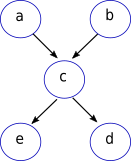
\includegraphics[width=.6\linewidth]{imgs/bayesnet1.png}
  		\caption{A Bayesian with 5 RVs.}
  		\label{fig:sub1}
	\end{subfigure}%
	\begin{subfigure}[t]{.33\textwidth}
  		\centering
  		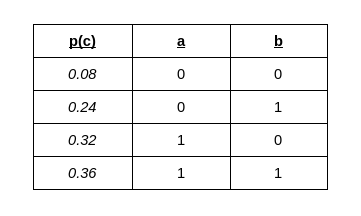
\includegraphics[width=.9\linewidth]{imgs/bayesnet2.png}
  		\caption{Tabular conditional probability $p(c |a , b)$.}
  		\label{fig:sub2}
	\end{subfigure}
	\begin{subfigure}[t]{.33\textwidth}
  		\centering
  		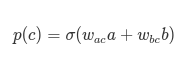
\includegraphics[width=.7\linewidth]{imgs/bayesnet3.png}
  		\caption{Conditional probability $p(c |a , b)$ given by a function over $a,b$.}
  		\label{fig:bayesnet}
	\end{subfigure}
	\caption{A sample Bayesian network with 5 binary nodes. (a) In the network RV $c$ is directly dependent on $a$, $b$ and thus $c$ is the child of its parents $a$, $b$. The RVs $d$, $e$ are the children of $c$. Since there is a path from $a$ to $e$, $a$ is an ancestor of its descended $e$. (b) The conditional probability of $p(c |a , b)$ in a tabular form. Another variant of the conditional probability $p(c |a , b)$ is given in (c). The probability is defined by the parameters $w_{ac}$, $w_{bc}$, and due to the sigmoid activation function $\sigma$ a network with such probability functions is called sigmoid belief network.}
	\label{fig:test}
\end{figure}

This is consistent with with the Markov property, since each node is only depend on its direct parents:

\[
p(x_i | x_{\setminus i}) = p(x_i | parents(x_i) ),
\]

where $x_{\setminus i} = \textbf{z} \setminus x_i$ and $\textbf{z} = (x_1, ... , x_n)$ is the state of the model.


A Bayesian network contains a simple conditional independence assertion, i.e. each variable is, given its parents, independent on all non descendants:

\[
p(\textbf{z}) = \prod_{x_i \in \textbf{z}} p(x_i | x_{\setminus i}) = \prod_{x_i \in \textbf{x}} p(x_i | parents(x_i) ) .
\]

This reduction provides (i.a from a computational perspective) an efficient way for learning/ parameter estimation and inference.
Given some observed variables, the evidences, the network can be used to compute the posterior probabilities and infer the most likely state of the hidden/ unobserved variables.
This process of computing the posterior distributions given the evidences is called probabilistic interference.

Thus a Bayesian network can be seen as a tool to simplify and apply the Bayes rule to complex problems.   

\subsection{Markov Random Field} \label{c:markovnet}

In contrast to Bayesian networks, Markov random fields are undirected graphical models, in which random variables are also represented by nodes but edges in this case indicate conditional dependencies \cite{Goodfellow-et-al-2016-Book}\cite{murphy2012machine}.
If two nodes $x_i$ and $x_j$ are connected by a edge, they are called each others neighbours.
Given all of their neighbours, two nodes $x_k$ and $x_m$ are independent on each other.
Thus an MRF can be seen as a model of the joint probabilities of RVs (see Fig. \ref{fig:markovnet1}).

As a result to reduce the complexities and redundancies of the probability distribution, instead of defining one probability distribution over all RVs, this allows a factorization of the probability distribution into fully connected partial graphs, so-called cliques:

\[
p(\textbf{z}) = \frac{1}{Z} \prod \phi (z_k)  ,
\]

where $Z$ is the normalization factor, so that $p(\textbf{z})$ is a valid probability distribution with $\sum_{\textbf{z}} p(\textbf{z}) = 1$ ($ \Rightarrow Z = \sum_z \prod \phi (z_k) $) and $\phi (z_k)$ is the partition function of the clique/ partial graph $z_k$.

The partition function $\phi (z_k)$ defines the potential of a clique, which indicates the likelihood of a state in the clique to be present.
The higher the clique potential of a state the more likely is that clique-state.
The clique potential for each state always has to be greater or equal to zero, but a common, computational beneficial choice is to represent each state with is purely positive value.

\begin{figure}
	\centering
	\begin{subfigure}[t]{.5\textwidth}
  		\centering
  		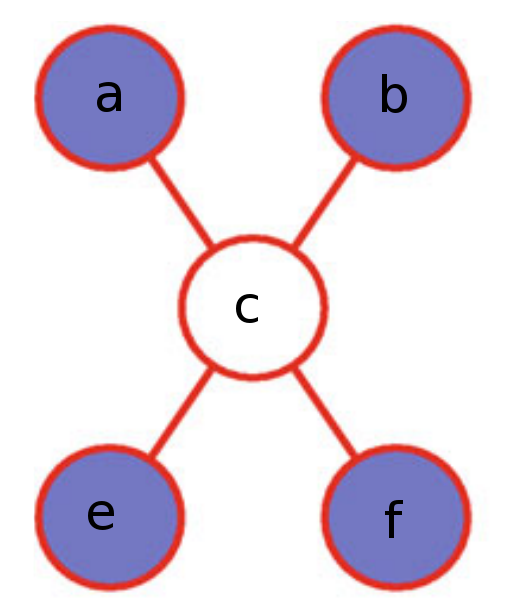
\includegraphics[width=.5\linewidth]{imgs/markovnet1.png}
  		\caption{A Markov network with with 5 nodes.}
  		\label{fig:markovnet1}
	\end{subfigure}%
	\begin{subfigure}[t]{.5\textwidth}
  		\centering
  		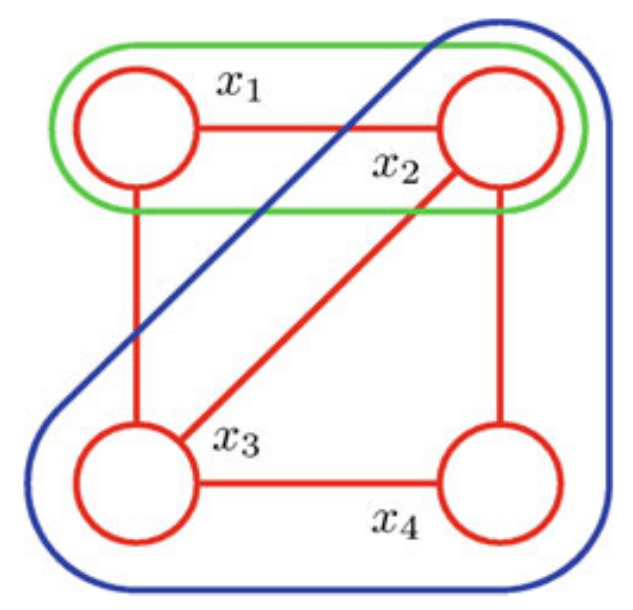
\includegraphics[width=.5\linewidth]{imgs/markovnet2.png}
  		\caption{Cliques in a Markov network}
  		\label{fig:markovnet2}
	\end{subfigure}
	\caption{(a) A Markov network with 5 nodes. The white node is dependent on all connected nodes (blue nodes). Given the blue nodes the white node is independent on any other node in the network. Given the white node all the blue nodes are independent on each other. (b) Two cliques in a Markov network. The blue clique is maximal, since no vertex can be added, which is fully connected to all others in the blue clique. The green one is not maximal, since the node $x_3$ could be added \cite{bishop2013pattern}.}
	\label{fig:markovnet}
\end{figure}


Usually the maximal (sized) cliques are chosen, since they contain all smaller sub-cliques and allow a finer factorization over those sub-cliques.
But depending on the concrete modelled problem, smaller clique sizes may be useful as well, e.g. Boltzmann machines usually are modelled with cliques of size two (see Fig. \ref{fig:markovnet2}).




\subsection{Energy-Based Models} \label{c:ebms}

One convenient way to model the clique potentials is to use an energy function $E(z_k)$ \cite{Goodfellow-et-al-2016-Book}: 

\[
\phi(z_k) = exp(- E(z_k))
\]

Models with exponentials over energy functions are called energy-base models (EBMs).

This is useful since, due to $exp(z_n)exp(z_m) = exp(z_n+z_m)$, the Energy of the complete graph can be decomposed into the sum of the energy of all cliques.
Because the exponential function is always positive ($exp(z) > 0$), the probability for each state is guaranteed to be greater than zero. 
This offers the freedom of choice of an arbitrary energy function $E(z_k)$, which can simplify optimization. 

A probability distribution given by an EBM is also called Boltzmann distribution, due to the similarity to statistical mechanics of gases in thermal equilibrium (and this is also where the Boltzmann machine get its name as presented in Chapter \ref{c:bms} ).

\subsection{Sampling} \label{c:sampling}

Often calculating the exact probability distribution or marginal distributions is a computational inefficient or untraceable problem \cite{Goodfellow-et-al-2016-Book} \cite{Petrovici2016}.
Sampling is a probabilistic solution to this problem, as it allows to approximate the target distribution nearly arbitrarily exact, and also turns calculating marginal probabilities into a by-product.  
An exemplary sampling of a Gaussian distribution is given in Figure \ref{fig:Sampling}.

Sampling can be described as the selection of a subset of individuals from a distribution to estimate properties of the complete distribution.
To select a representative subset, the samples have to be unbiased of external influences, such as the the sampling procedure or problems in data collection.
This can be particularly hard since it may need infinite data, computational or temporal resources.
This where graphical models are especially useful, since they often facilitate the task of drawing samples from a distribution.

\begin{figure}
	\centering
    	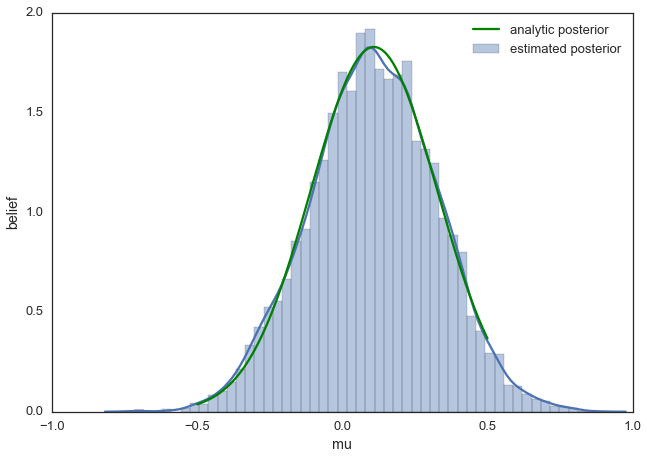
\includegraphics[width=0.4\textwidth]{imgs/sampling.png} 
    \caption{Sampling a Gaussian distribution. The number of samples in an interval approximates the true density function. As more samples are drawn, the approximation of the density function will be more exact \cite{sampleFD}.}
	\label{fig:Sampling}
\end{figure}



\paragraph{Ancestral Sampling} For directed graphical models, such a Bayesian networks, there is a simple and efficient procedure called ancestral sampling, which can produce samples from the probability distribution represented by the model \cite{Goodfellow-et-al-2016-Book}. 
The basic idea is to sort the variables $x_n$ in the graph into a topological ordering, so that for all $i$ and $j$, $j$ is greater than $i$ if $x_i$ is a descendant of $x_j$. The variables can then be sampled in this order.

The topological sorting operation guarantees that the conditional distributions are valid and one can sample from them in order.

\paragraph{Markov Chain Monte Carlo} If the probability distribution is represented by an undirected model, Markov Chain Monte Carlo (MCMC) methods can be used \cite{Goodfellow-et-al-2016-Book}. 
MCMC methods interpret the model as a Markov chain, and work best in an irreducible and aperiodic chain, that is when no state in the undirected model has zero probability.

The basic idea is to begin in a state $z$ with some arbitrary value. 
Then for some time $z$ is repeatedly randomly updated using the, by the model given, transition distribution $T(z',z)$. 
Given enough update steps (possibly an infinite number) the network states will have reached a distribution, which does not change any more (even so the individual states might do, the relative number of time spend in on state becomes constant).
Such a distribution is referred to as stationary distribution or equilibrium distribution (due to its similarity to particle physics).
Eventually $z$ becomes a fair sample of $p(z)$, which is equivalent to the stationary distribution of the Markov chain.

To get more than one sample, one can run more Markov chains in parallel, each initialized with a random starting state. 
Another method is to run only one Markov chain, run it for some time to allow the Markov chain to reach its equilibrium, and than take samples after different timesteps.
Those approaches need the Markov chain to reach its equilibrium distribution, which is usually done, by letting it run for some burn in time.
But there is no guaranty, that the Markov chain has settled in the given timespan.    
Another problem with the second approach is, that since it can be hard to escape probable states, and when not run for an infinite timespan, more likely states can be over represented and less likely states under represented, if they did not occur or over represented if they did occur.  

\paragraph{Gibbs sampling} Gibbs sampling is a commonly used MCMC algorithm \cite{Goodfellow-et-al-2016-Book}. The basic idea to perform the transition from one state to another in accordance with $T(z',z)$ is, to sample a single variable $x_i$ only conditioned on its neighbours. 
Several variables can be sampled at the same time as long as they are conditionally independent given all of their neighbours.

\section{Neural Networks} \label{c:NNs}

In this section we will examine the foundations of natural and artificial neural networks (NNs).
At first we will look at the mechanism behind natural neural networks in the brain.
We will then describe different artificial models, starting with models working at discrete time steps and then models, which work in continuous time.
To distinguish those, throughout this thesis we will refer to models working at discrete time steps as \textit{artificial neural networks} (ANNs) and models working in continuous time as \textit{spiking neural networks} (SNNs).

\subsection{Natural} \label{c:natural}
\subsubsection{Brain} \label{c:brain}

The human brain is the main organ of the human central nervous system and with a weigh of about 1.2 - 1.4 kg (2\% of the total body weight) and a power consumption around 20 Watts (20\% of the total human power consumption), it is thought to be mainly responsible, for what's commonly called human intelligence \cite{gerstner2014neuronal}\cite{Byrne1997}.  

\begin{figure}
	\centering
    	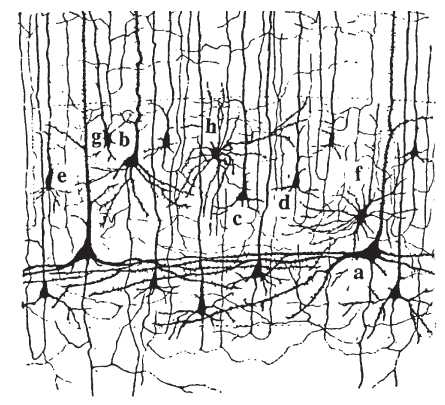
\includegraphics[width=0.4\textwidth]{imgs/brain.png} 
    \caption{A small section in the Brain. The neurons $a$ - $g$ are connected to other neurons in a complex network \cite{gerstner2014neuronal}.}
	\label{fig:brain}
\end{figure}

A human constantly brain performs tasks as learning, memory, self-control, planing, reasoning, abstract thought, motor control, vision and language.
We can localize different specialized regions in the brain which are involved in a given tasks. 

Even so different regions are involved in different tasks, the basic building blocks of the brain are astonishingly uniform. 
It is mainly composed of neurons, glial cells and blood vessels.
While the neurons cells are the main computational unit, the other constituents are required for structural stabilization and energy support.
A single neuron can perform only quite simple operations but, the human brains contains $10^{12}$ neurons and each single neuron is interconnected with $10^{4}$ other neurons.
The resulting complex neural network with roughly $10^{15}$ neural connections are the main component for human intelligence and enable complex task as scene understanding, language processing and motion planing. A small section of a neural network recorded in a human brain is shown in Figure \ref{fig:brain}. 

\subsubsection{Neuron} \label{c:natneuron}

Neurons are the main information processing unit in the brain\cite{gerstner2014neuronal}\cite{Byrne1997}. 
Information is primarily processed through chemical and electrical signals.

A neuron, which is a specialized kind of (biological) cell, is separated from its surroundings by a cell membrane.   
Due to ion concentration differences between the interior and the exterior of the cell, there are potential differences at the cell membrane, which are refereed to as the membrane potential. 
Ion channels, often voltage gated, in the cell membrane allow positive and negatively charged ions to flow from the inside to the outside and from the outside to the inside of the cell.
This can lead to an increase (de-polarization) or decrease (hyper-polarization) of the membrane potential.
The ion flow is primarily determined by the charge difference at the membrane (reversal potential), the ion concentration differences (nernst potential) and ion pumps actively pumping ions across the membrane.
The membrane of a neuron at rest, with an equal influx and outflow of ions neutralizing each other, has usually a resting/equilibrium potential of -65 mV. 

Each singe neuron can be divided into three functional distinct parts: the dendrites, the soma and the synapses (see Fig. \ref{fig:neuron}).

\begin{figure}[h]
	\centering
    	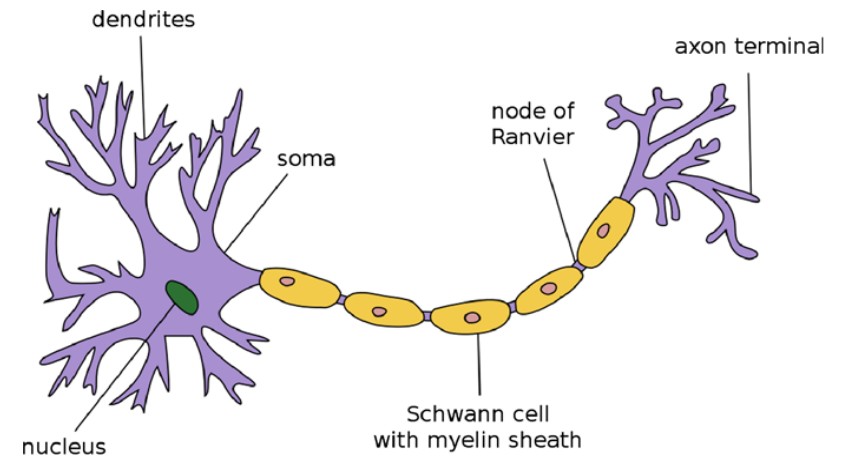
\includegraphics[width=0.6\textwidth]{imgs/neuron.png} 
    \caption{A schematic view of a natural neuron. Other neurons are pre-synaptic connected via the dendrites. The signals are then forwarded and accumulated in the soma and from there on via the in myelin sheath cover axon to the axon terminal and the out going synapses \cite{neuronImg}.}
	\label{fig:neuron}
\end{figure}

The dendrites are thin, complexly branching structures emerging the cell body/ soma.
They are the primary access for signals of preceding neurons through their synapses. 
These signals can polarize or depolarize the part of the dendrites and so inhibit or promote a spike. 

The cell body or soma, which encompasses the nucleus, accumulates all polarizations from the dendrites and if the accumulation exceeds a "pseudo" threshold, usually around -55 mV, certain ion channels become more active, which allows an influx of positively charged ions and a spike emerges.

The spike is propagated across the axon to the axon terminal where it distributed to the dendrites of other subsequent (post-synaptic) neurons via the synapses, where they in turn can evoke (post-synaptic) potentials.
The axon is often covered by a fatty substance, the myelin, to regulate and improve the conductivity.

Synapses can be divided into two different categories: Electrical, which communicate with other neurons with direct electrical connections and chemical which use chemical compounds.
Probably due to their more diverse form of signal exchange, almost exclusively all synapses found in the brain have a chemical nature.

\subsubsection{Learning} \label{c:natlearning}

The exact mechanisms behind learning in the brain are still mostly unknown \cite{gerstner2014neuronal}\cite{Byrne1997}\cite{Markram2012}.
Neural plasticity is often considered be to one of the methods behind learning. 
It describes the ability of the brain to change and reorganize the structure of brain, build new and alter connections.  

\paragraph{Synaptic Plasticity} \label{c:synplasiticity}
specifies the changes to the synaptic strength, which is often associated with task learning and memory (in contrast to learning in brain, which is the general mechanism of altering the information processing in the brain, task learning describes the actual learning and remembering of a task). 

Synaptic plasticity builds on the principle that temporally and locally correlated neural activity  can lead to synaptic changes.
It is often further divided in \textbf{short-term plasticity} which acts on a time scale one milliseconds to a minutes and \textbf{long-term plasticity}, lasting minutes or more.


\paragraph{"What fires together, wires together"} \label{c:hebb}
A principle which generalizes these principles is the Hebbian principle or Hebbian rule.
It is often commonly summarized as "Cells that fire together, wire together".
Hebb originally stated it as follows: "When an axon of cell $A$ is near enough to excite a cell $B$ and repeatedly or persistently takes part in firing it, some growth process or metabolic change takes place in one or both cells such that $A$'s efficiency, as one of the cells firing $B$, is increased."\cite{hebb19680}.
Meaning, the more often $A$ is active directly before $B$, the more likely $A$ will have contributed to $B$'s spike and the more causal $B$ will become of $A$/ $A$ and $B$ become associated.
This can be mathematically expressed as
\[
\Delta w_{ab} = \eta v_a v_b ,
\]
where $\Delta w_{ab}$ describes the change of the synaptic weight between the pre-synaptic neuron $A$ and the post-synaptic neuron $B$. 
$v_a$ and $v_b$ describe the activity of $A$ and $B$, respectively and $\eta$ is some positive learning rate. 

While this describes the classical Hebbian principle, often different algorithms processing the neural activity of two connected neurons are summarized and labelled as general Hebbian learning algorithms.
Such algorithms can in be general formalized as
\[
\Delta w_{ab} = F( v_a, v_b) , 
\]
where $F$ is a function describing the weight change conditioned on the neural activities \cite{gerstner2014neuronal}.     
This formulation allows a more complex processing of the neural activity and implementations as e.g. the original formulation of the Hebbian principle as well as the anti-Hebbian rule. 

\subsection{Artificial neural networks} \label{c:ann}

The first artificial neural network models performed computations at discrete time slices.
While it simplifies the neuron model a lot, it makes them exceptionally easy to handle on most processors, which also work at a discrete tact rate.

\subsubsection{Perceptron} \label{c:perceptron}

The perceptron, also called Rosenblatt Perceptron, was invented in the late 1950s by Frank Rosenblatt \cite{rosenblatt1958perceptron}. 
It was one of the first artificial neural networks, and can be seen as the foundation of most of the modern (deep) neural networks as well as linear discriminating classifiers. 

\paragraph{Model} \label{c:permodel}

The perceptron loosely models a neuron with a multi-dimensional input and a single output (see Fig. \ref{fig:perceptron}). 

\begin{figure}
	\centering
    	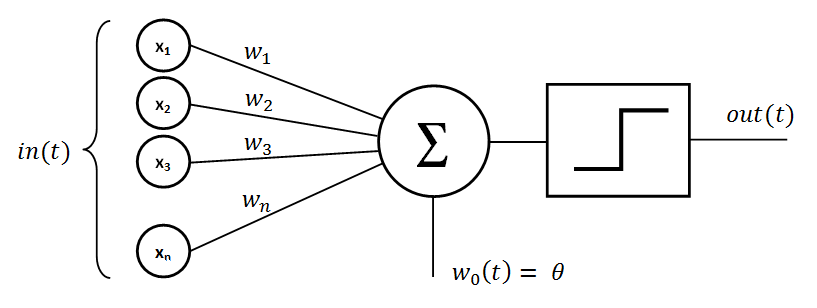
\includegraphics[width=0.8\textwidth]{imgs/percept.png} 
    \caption{Structure of a perceptron. The input $in(t)$ is set at the input variables $x_i$ and the multiplied with the corresponding synaptic weight $w_i$ and accumulated. In addition a threshold offset $\theta$ is added. On the sum the step-function is applied i.e. the output $out(t)$ is $1$ if the sum is greater $0$ and $0$ if the sum is smaller $0$ \cite{perceptronImg}.}
    % https://github.com/cdipaolo/goml/tree/master/perceptron
	\label{fig:perceptron}
\end{figure}

Be $\textbf{x} \in \mathbb{R}^n$ the input of dimension $n$ and $\textbf{w}\in \mathbb{R}^n$ the $n$-dim vector describing the synaptic weights, then each $x_i$ is multiplied by it's synaptic weight $w_i$ and then accumulated/summed up:
\[
\sum x_i w_i = \textbf{x}^\intercal \textbf{w}.
\] 

If the sum exceed a threshold $b$, often referred to as the bias, the perceptron "fires" and the output $y$ is set to $1$ and otherwise it is set to $0$.

\[
	f = 
		\begin{cases}
			1, \text{  if  } \textbf{x}^\intercal \textbf{w} + b > 0  \\
			0, \text{  if  } \textbf{x}^\intercal \textbf{w} + b \le 0
		\end{cases}	
\]

One simplification is to append the bias $b$ to the weight vector $\textbf{w}' = (b , w_1, ... , w_n)$ and to extend the input dimension by a constant one $\textbf{x}' = (1, x_1 , ... , x_n)$ .
This allows us to handle the bias as a simple synaptic weight, and thus we will cease to  model it explicitly and further on.

\[
	f = 
		\begin{cases}
			1, \text{  if  } \textbf{x}'^\intercal \textbf{w}'> 0  \\
			0, \text{  if  } \textbf{x}'^\intercal \textbf{w}' \le 0
		\end{cases}	
\]



Using the heaviside step function $\varphi_{step}$, the perceptron calculation rule can be rewritten as 
\[
	f = \varphi_{step}(\textbf{x}'^\intercal \textbf{w}) .
\]   

\paragraph{Decision Function} \label{c:perdecision}

This equation can be interpreted as a linear discrimination function, where $\textbf{w}$ defines a hyper plane in the data space, diving it into two half spaces. 
Two exemplary linear discrimination function in data space are given in Figure \ref{fig:discrimation}.
This separation of the data space into distinct sub spaces is often regarded to as classification. 
While a perceptron with a linear decision function only allows quite simple discrimination, more complex decision functions can be chosen e.g. multi layers perceptrons combine simple function into more complex ones. 

\begin{figure}
	\centering
	\begin{subfigure}[t]{.45\textwidth}
	 	\centering
  		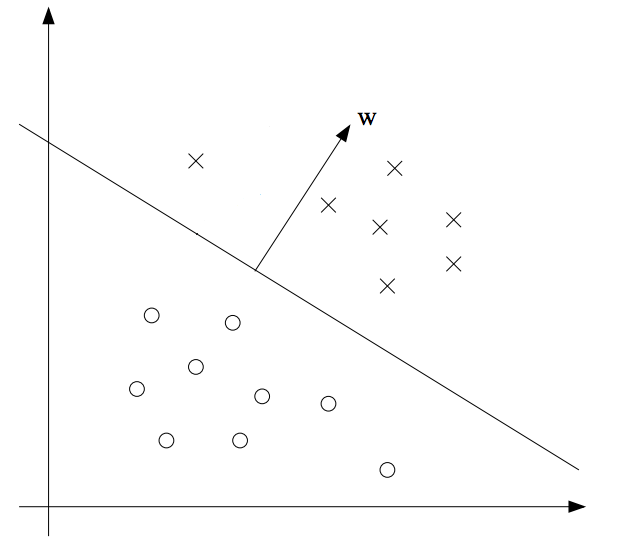
\includegraphics[width=.9\linewidth]{imgs/percept_discr1.png}
  		\caption{}
	\end{subfigure}
	\begin{subfigure}[t]{.45\textwidth}
	 	\centering
  		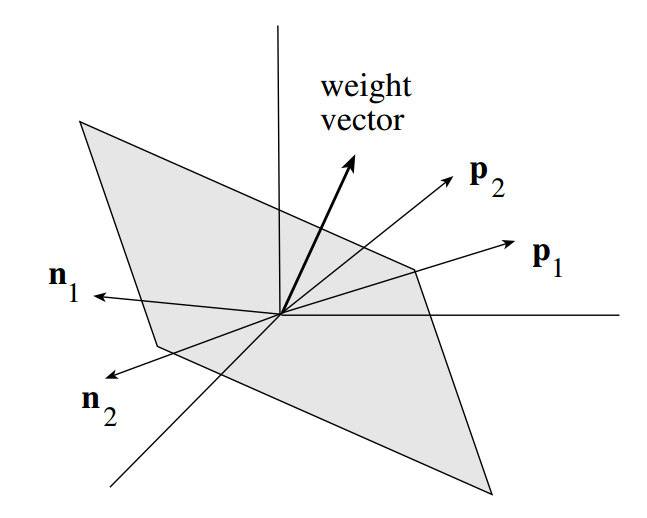
\includegraphics[width=.9\linewidth]{imgs/percept_discr2.png}
  		 \caption{}
	\end{subfigure}
    \caption{The discrimination function of a perceptron. The discrimination function has the shape of a linear hyper plane in data space and it defined by the synaptic weight-vector $\textbf{w}$. It divides the data space and thus the data samples into two subspaces, the positive space $\textbf{x}^{\intercal}\textbf{w} > 0$ and the negative space $\textbf{x}^{\intercal}\textbf{w} < 0$. In (a) the discrimination function is given in a two-dimensional data space and in (b) in a three-dimensional data space.}
	\label{fig:discrimation}
\end{figure}


\paragraph{Perceptron Learning} \label{c:perlearning}

Be $\textbf{X}$ a set of data-points and $\textbf{Y}$ their corresponding label and $\mu$ a learning rate. 

For a sample $x \in \textbf{X}$  and $y \in \textbf{Y}$ and $\tilde{y}$ the output of the perceptron, one update step can be described as:
\[ 
	w = w + \Delta w
\]
, where 
\[
	\Delta w = \mu (\tilde{y}-y) x .
\]
Thus the learning algorithm can be described as follows:

\begin{enumerate}
	\item Initialize $w$ randomly.
	\item Select a data sample and calculate its output.
	\item Calculate $\Delta w$ and update the weights.
	\item Performed steps 2.-3. until all data samples are correctly classified i.e. $\tilde{y} = y$ or a predetermined number of iterations have been completed
\end{enumerate}


\subsubsection{Mutlilayer-Perceptron} \label{c:mlp}

While the perceptron models a single neuron, a multi-layer perceptron, consisting of stacked perceptrons, can be seen as an extension of the model to neural networks and by doing so overcoming the perceptrons disadvantage to only discriminate linearly \cite{rumelhart1985learning}\cite{Goodfellow-et-al-2016-Book}. 

\paragraph{Model architecture} \label{c:mlparch}

A MLP is built up of multiple consecutive layers (see Fig. \ref{fig:mlp}).

Each layer combines multiple perceptrons to map a multi-dimensional input $\textbf{x} \in \mathbb{R}^n$ to a multi-dimensional output $\textbf{y} \in \mathbb{R}^m$.
The output $\textbf{y}$ of the layer is composed of the $m$ individual outputs $y_i$ of the perceptrons in the layer on the same input.


A layer is defined by:
\begin{enumerate}
	\item The input dimension $n$,
	\item The output dimension $m$ (which can be seen as the number of individual perceptrons in the layer),
	\item The Weight matrix $W \in \mathbb{R}^{nxm} $ defining the weights between the synaptic connections,
	\item The activation function $\varphi : \mathbb{R}^m \rightarrow \mathbb{R}^m $.
\end{enumerate}

The output $\textbf{y}$ of the layer is calculated as:
\[
\textbf{y} = \varphi(x^\intercal W)
\]

Each element $y_i \in \textbf{y}$ can be interpreted as the output of a perceptron given the input $\textbf{x}$ and the synaptic weights $w_i \in W = (w_1, ... , w_n)$.

By using the output of a previous layer $l$ as input for a next layer $l+1$, several layers can be stacked up: 
\[
\textbf{y}^{l+1} = \varphi ((\textbf{y}^{l})^\intercal W^{l+1} ) ,
\]
where the superscript index represents the layer number. 

Modelled like this, the output is always forwarded to the next layer, so there are no cycles in the information flow of the network.
Such a network with only forward connections is called feed-forward network (in contrast to recurrent networks such as Boltzmann machines, which are introduced in Chapter \ref{c:bms} and allow information to be forwarded in cycles).

\begin{figure}
	\centering
    	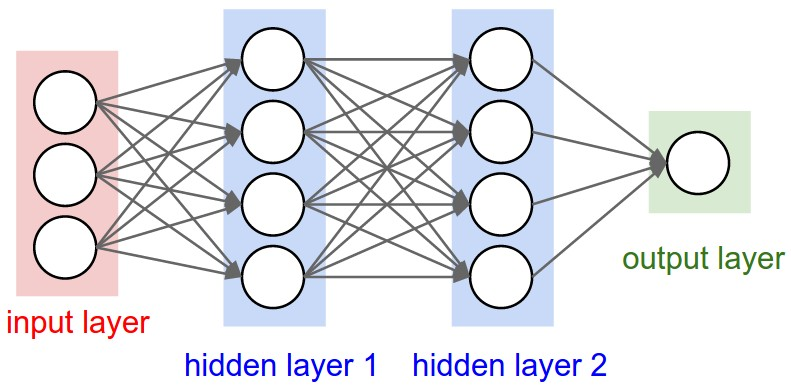
\includegraphics[width=0.6\textwidth]{imgs/mlp.jpeg} 
    \caption{A schematic multi layer perceptron with three layers \cite{mlpImg}.}
	\label{fig:mlp}
\end{figure}



\paragraph{Activation functions} \label{c:mlpact}

The activation function $\varphi$ can be basically arbitrarily chosen. 
There different activation functions, with different attributes, have been proposed, which also have proven to perform well on certain tasks:

\begin{itemize}
	\item Step-function: $\varphi_{step}(x_i) = \begin{cases} 1, & \text{if  } x_i > 0 \\ 0, & \text{if  } x_i \le 0  \end{cases}$
	\item Sigmoid-function: $\sigma(x_i) = \frac{1}{1 + e^{-x_i}}$ 
	\item Softmax-function: $\varphi_{softmax}(x_i) = \frac{e^{x_i}}{\sum_k e^{x_k}}$ 
	\item Sign-function: $\varphi_{sign}(x_i) = \begin{cases} 1, & \text{if  } x_i > 0 \\ -1, & \text{if  } x_i \le 0  \end{cases}$
	\item Tanh-function: $tanh(x_i) = \frac{e^{x_i} - e^{-x_i}}{e^{x_i} + e^{-x_i}}$
	\item ReLU-function $\varphi_{ReLU}(x_i) = max(0, x_i)$
\end{itemize}

A visualization of those functions is given in Figure \ref{fig:activations}.

\begin{figure}
	\centering
    	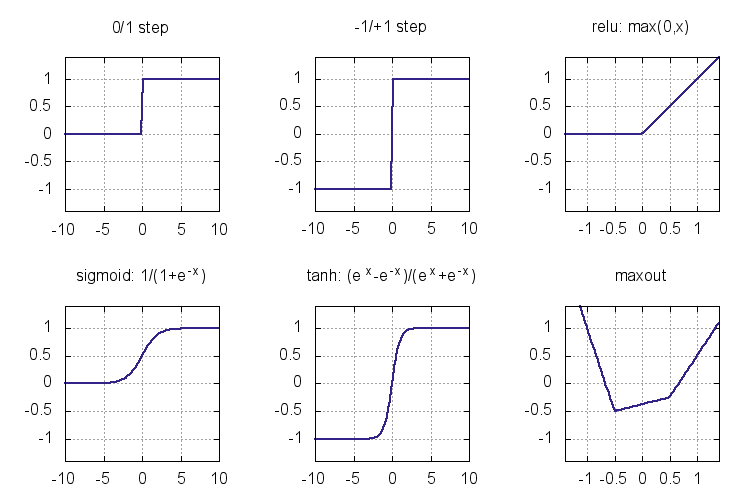
\includegraphics[width=0.8\textwidth]{imgs/act_fun.png} 
    \caption{The output of different activation functions plotted given the input.}
    % http://knet.readthedocs.io/en/latest/mlp.html
	\label{fig:activations}
\end{figure}

Different activation functions describe the behaviour of the neurons on the input data.
This is very similar to choosing different neuron models for spiking neural networks.


\paragraph{Error functions} \label{c:mlperr}

In machine learning, to validate the quality of the model an error function/cost function is used.
The error function gives a quantification of the performance of the model on a given task.
Thus the primary goal of a learning algorithm is to reduce the error on its task.
Hereby it is important to note that the main error function is often primarily task dependent and rather independent on the learning algorithm used.  

To compare the outputs $\tilde{\textbf{y}}$ of the network with parameters/weights $\theta$ to the correct data-labels $\textbf{y}$ some of the most used error function or cost function $E(\textbf{y},\tilde{\textbf{y}} | \theta)$ are:.

\begin{itemize}
	\item Mean squared error: $MSE = \frac{1}{N} \sum_{i=1}^N (\tilde{\textbf{y}}_i - \textbf{y}_i)^2 $
	\item Cross entropy: $CE = - \frac{1}{N} \sum_{i=1}^N [ \textbf{y}_i \log \tilde{\textbf{y}}_i + (1 - \textbf{y}_i) \log (1 - \tilde{\textbf{y}}_i)]$
\end{itemize}

\paragraph{Backpropagation} \label{c:backprop}

In order to reduce the error $E$ on a task, the parameters $\theta$ of the model can be changed.
This modification of the parameters is often referred to as learning.
Thus the objective is to get parameters $\theta^*$ which form a (global) minimal point in the error function. 
Different optimization algorithms can be used to achieve this objective, but the most common class of algorithms use the gradient of the error function with respect to the weights, to determine the contributions of the weights to the error and thus reduce the error and reach a minimal point.
Gradient descent calculates the gradient for the parameters, and by following the negative gradient direction the weights are updated.

Since MLPs have a clearly defined structure, using the chain rule of calculus, the gradient descent update rule can be simplified to an iterative procedure called backpropagation (backprop)  \cite{rumelhart1985learning}\cite{Goodfellow-et-al-2016-Book}.

We define the output $y_j$ of neuron $j$ as
\[
	y_j = \varphi(net_j) = \varphi(\sum_{k=1}^n w_{kj} y_k) .
\]
 
The partial derivative of the error function $E$ with respect to a weight $w_{ij}$ can be simplified by the repetitive application of the chain rule:
\[
	\frac{\partial E}{\partial w_{ij}} = \frac{\partial E}{\partial y_j} \frac{\partial y_j}{\partial net_j} \frac{\partial net_j}{\partial w_{ij}} .
\]
 
Where the single factors of the derivation can be resolved to:
\[
	\frac{\partial net_j}{\partial w_{ij}} = \frac{\partial}{\partial w_{ij}} ( \sum_{k=1}^n w_{kj} y_k ) = y_k
\]
and 
\[
	\frac{\partial y_j}{\partial net_j} =  \frac{\partial \varphi(net_j)}{\partial net_j} = \varphi'(net_j).
\]


This just leaves the first factor $\frac{\partial E}{\partial y_j}$. It can be further divided into two simple cases:
1. The neuron $j$ is in the output layer:
\[
\frac{\partial E}{\partial y_j} = \frac{\partial E(y_j)}{\partial y_j} = E'(y_j).
\] 

2. The neuron $j$ is not in the output layer and $L$ is the layer above neuron $j$:
\[
\frac{\partial E}{\partial y_j} = \sum_{l \in L}( \frac{\partial E}{\partial net_l} \frac{\partial net_l}{\partial y_j} )  = \sum_{l \in L}( \frac{\partial E}{\partial net_l} w_{jl} ).
\] 

We define 
\[
\delta_l = \frac{\partial E}{\partial net_l} = \frac{\partial E}{\partial y_l} \frac{\partial y_l}{\partial net_l} =
\begin{cases}
E'(y_l) \varphi'(net_l), & \text{  if } j \text{ is an output neuron} \\
(\sum_{k \in K} \delta_k w_{lk}) \varphi'(net_l), & \text{  if } j \text{ is not an output neuron.}
\end{cases}
\]

This all concludes to 
\[
\frac{\partial E}{\partial w_{ij}} = 
\begin{cases}
E'(y_j) \varphi'(net_j) w_{ij}, & \text{  if } j \text{ is an output neuron} \\
(\sum_{l \in L} \delta_l w_{jl}) \varphi'(net_j) w_{ij}, & \text{  if } j \text{ is not an output neuron.}
\end{cases}
\]

An update step for a weight $w_{ij}$ can now be written as
\[
w_{ij} = w_{ij} - \mu \Delta w_{ij} = w_{ij} - \mu \frac{\partial E}{\partial w_{ij}},
\]
with a learning rate $\mu$.

\subsubsection{Convolutinal Neural Networks} \label{c:cnns}

Convolutional neural networks (CNN) exploit spacial relations and the compositional structure of the input data to regularize the complexity of the neural network by putting further constrains on the architecture of those nets.
This makes them easier to train and allows greater generalization on fewer training samples.
It is implemented by having only partially connected layers with shared connection weights, instead of fully connected nets \cite{lecun1989backpropagation}\cite{Goodfellow-et-al-2016-Book}.    

\paragraph{Convolution} \label{c:convolution}

As the name suggests CNNs perform a convolution operation \cite{Goodfellow-et-al-2016-Book}. The one dimensional convolution operation $c$ is defined as
\[
c(t) = (a * b)(t) = \int_{- \infty}^{\infty} a(x)b(t-x) dx.
\]
In this equation $a$ is usually called the input and $b$ the kernel of the convolution. The result $c$ is often referred to as the feature map.

Since recorded data (e.g. images, speech) is often discretized, we extend the convolution to discrete data
\[
c(t) = \sum_{x = - \infty}^{\infty} a(x)b(t-x).
\]
Whereas convolution is originally only defined over the one-dimensional temporal dimension, it can be also applied to multiple arbitrary dimensions, e.g. two dimensional images $I$
\[
C(i,j) = \sum_m^M \sum_n^N I(m,n) K(i - m, j -n).
\]
In this case the kernel matrix $K \in \mathbb{R}^{M \times N} $ as well as the feature map $C$ also spans multiple dimensions.
A more intuitive way to rewrite this equation can be achieved by using the commutative nature of the convolution operation
\[
C(i,j) = \sum_m^M \sum_n^N I(i - m,j - n) K(m, n).
\]
Similar to the convolution is the cross correlation, which is basically a convolution without a flipped kernel
\[
C(i,j) = \sum_m^M \sum_n^N I(i + m,j + n) K(m, n).
\]
Due to this similarity the terms convolution and cross correlation are often used ambiguously (see Fig. \ref{fig:conv} for a sample cross correlation over a two dimensional input).

\begin{figure}
	\centering
    	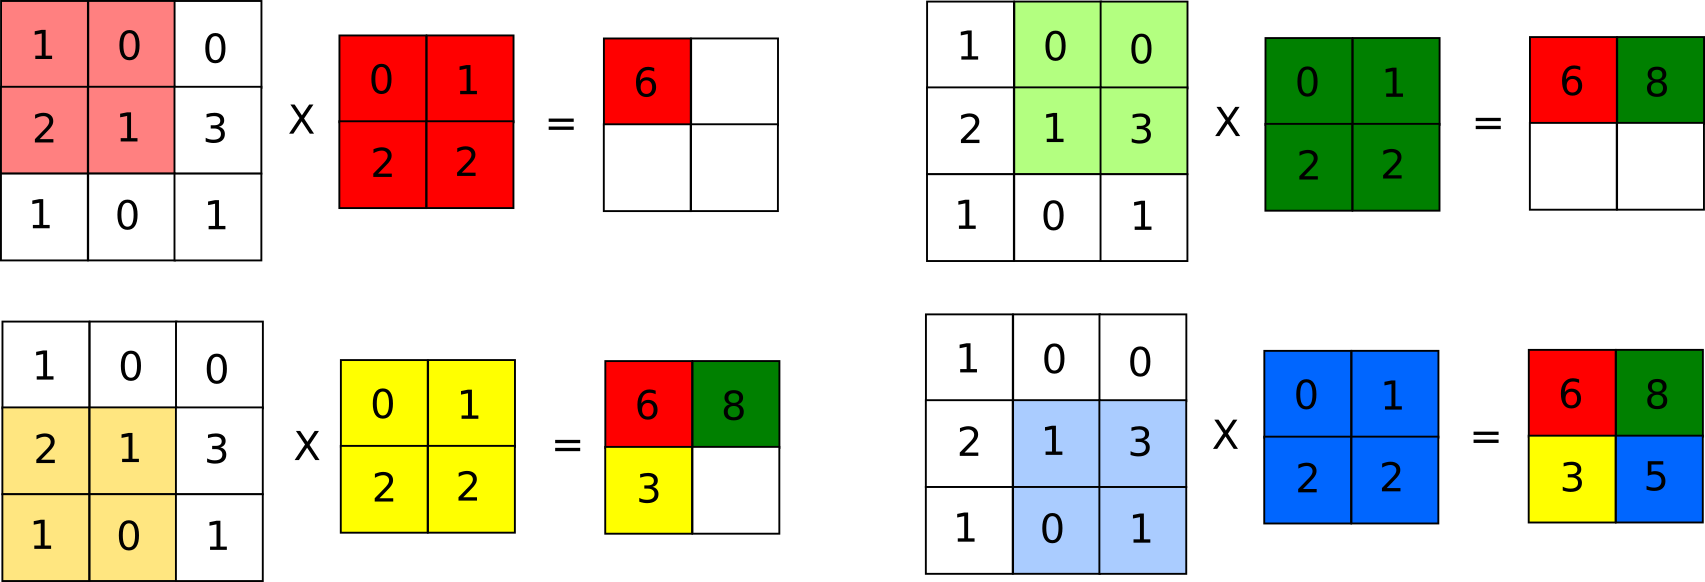
\includegraphics[width=0.8\textwidth]{imgs/convolution.png} 
    \caption{A cross correlation of a $3\times3$ image matrix with a $2\times2$ kernel without stride and padding. The result is a $2\times2$ feature map.}
	\label{fig:conv}
\end{figure}

\paragraph{Convolution Layers} \label{c:convlayers}

In neural networks convolution is implemented in the so-called convolution layer, where the convolution operation with a learnable kernel matrix $K$ is applied. An input given as an 3D tensor $Y$ be composed of $m$ 2D feature maps. Each feature map has the dimension $s \times t$. In the input layer, $m$ is for example the number of color channels (3 in case of an RGB image), and $s$ is the width and $t$ the height of the input image. A discrete convolution with a $(M , P , Q)$ filter matrix $K_j$ at position $(x,y)$ is then defined as : 
\[
y_{i}^{jxy} = \sigma(\sum_M \sum_{p=-\frac{P}{2}}^{\frac{P}{2}} \sum_{q=-\frac{Q}{2}}^{\frac{Q}{2}} w_{ij}^{mpq} y_{(i-1)}^{m(x+p)(y+q)}) .
\]
where $w_{ij}^{mpq}$ is the value at position $(m,p,q)$ of the $j$th Kernel matrix $K_j$ in the $i$th layer and $y_{i}^{jxy}$ is the entry in the $j$th 2D-feature map in the $i$th layer at position $(x, y)$.\\
In a typical layer the weights $w_{ij}^{mpq}$ of all Kernel matrices $K_j$ in all layers $i$ are the free parameters that have to be learned. Other so called hyper-parameters which have to be determined are the number $j$ of Kernel matrices at each layer $i$, their stride size, defining by how much you want to shift your filter at each step, and therefore the output dimension of the layer.
Recent state-of-the-art systems have mostly reached the common consensus, of choosing a stride of $1$, which we have adapted throughout this thesis \cite{simonyan2014very}.


%\begin{figure}
%	\centering
%	\begin{subfigure}[t]{.20\textwidth}
%  		\centering
%  		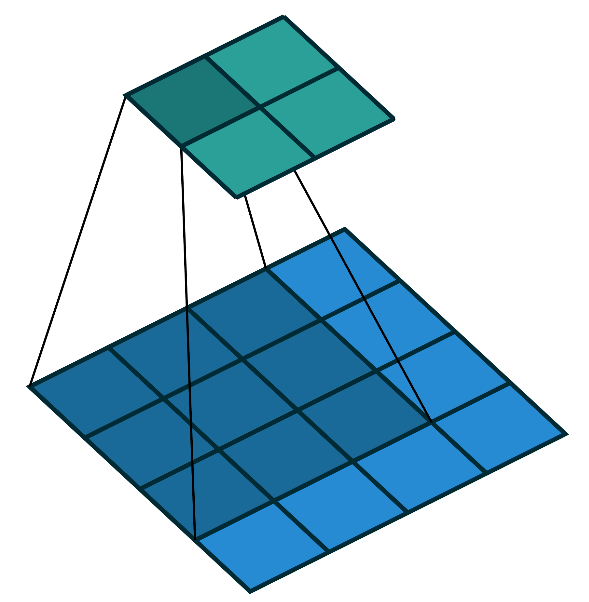
\includegraphics[width=.8\linewidth]{imgs/conv_layer1.png}
%  		\caption{A subfigure}
%  		\label{fig:sub1}
%	\end{subfigure}%
%	\begin{subfigure}[t]{.20\textwidth}
%  		\centering
%  		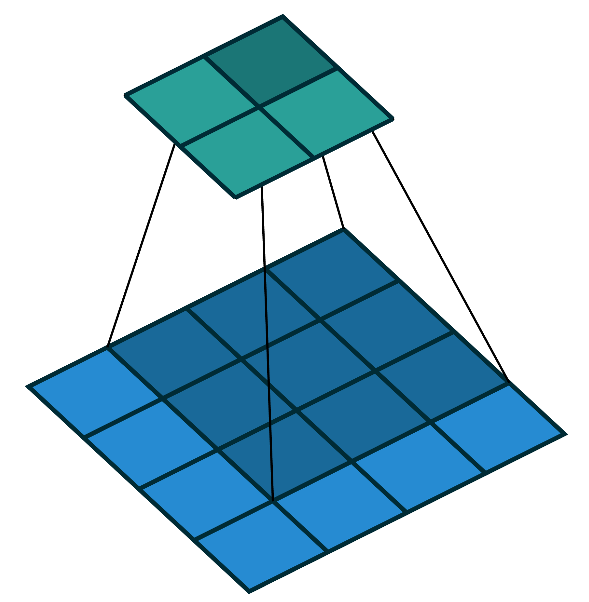
\includegraphics[width=.8\linewidth]{imgs/conv_layer2.png}
%  		\caption{A subfigure}
%  		\label{fig:sub2}
%	\end{subfigure}
%	\begin{subfigure}[t]{.20\textwidth}
%  		\centering
%  		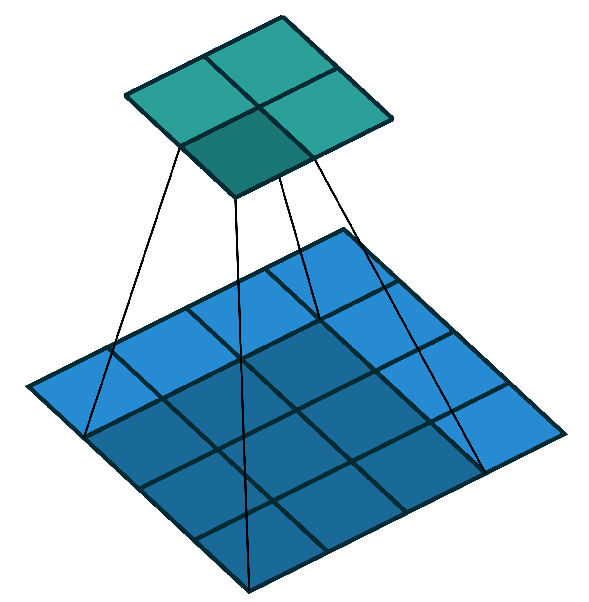
\includegraphics[width=.8\linewidth]{imgs/conv_layer3.png}
%  		\caption{A subfigure}
%  		\label{fig:sub3}
%	\end{subfigure}
%	\begin{subfigure}[t]{.20\textwidth}
%  		\centering
%  		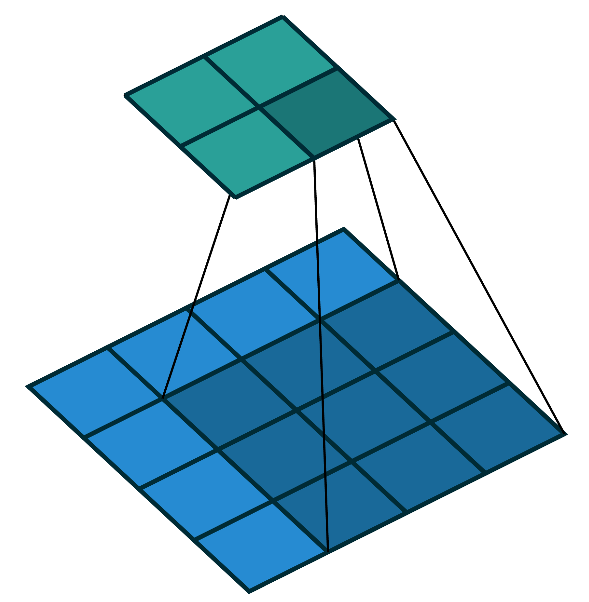
\includegraphics[width=.8\linewidth]{imgs/conv_layer4.png}
%  		\caption{A subfigure}
%  		\label{fig:sub4}
%	\end{subfigure}
%	\caption{A figure with two subfigures}
%	\label{fig:test}
%\end{figure}


\paragraph{Architecture} \label{c:cnnarch}

The most common architectures for CNNs are built up from stacks of alternating convolutional and pooling layers. 
After those layers, fully connected layers are used as a classifier to assign labels to the extracted features \cite{NIPS2012_4824}\cite{simonyan2014very}\cite{szegedy2015going}.
A sample architecture is given in Figure \ref{fig:convarcitecuture}.

\begin{figure}[h!]
	\centering
    	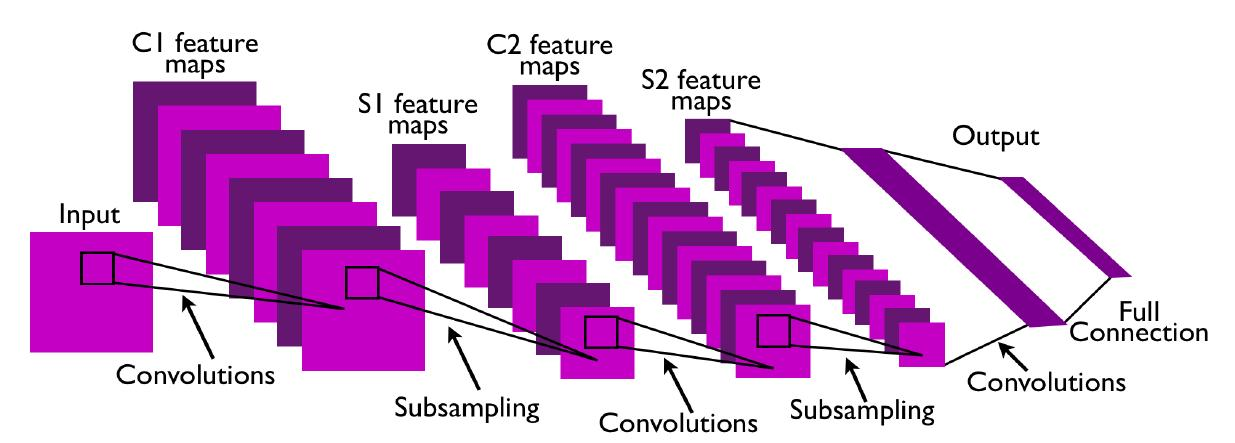
\includegraphics[width=0.8\textwidth]{imgs/cnn_architecture.jpg} 
    \caption{Typical architecture of a convolutional neural network with two convolution-pooling stages \cite{cnnarchImg}.}
	\label{fig:convarcitecuture}
\end{figure}

\paragraph{Training} \label{c:cnntraining}

% http://jefkine.com/general/2016/09/05/backpropagation-in-convolutional-neural-networks/

The training is performed applying the backprop algorithm to convolution:
\[
\frac{\partial E}{\partial w_{ij}^{mpq}} = \sum_{m'} \sum_ {q'}  \sum_{p'} \frac{\partial E}{\partial y_i^{m' p' q'}}  \frac{\partial y_i^{m' p' q'}}{\partial w_{ij}^{mpq}}  = \sum_{m'} \sum_ {q'}  \sum_{p'} \delta_i^{m' p' q'}  \frac{\partial y_i^{m' p' q'}}{\partial w_{ij}^{mpq}}.
\] 
By applying the chain rule this can be rewritten as
\[
\frac{\partial E}{\partial w_{ij}^{mpq}} = \sum_{m'} \sum_ {q'}  \sum_{p'} \delta_i^{m' p' q'}  \varphi(y_{i-1}^{m'-m, p'-p, q'-q}) = \delta_i^{m p q}  * \varphi(y_{i-1}^{-m, -p, -q}).
\] 
Another more intuitive update rule is given by defining the contribution to the error of an single weight as
\[
\frac{\partial E}{\partial y_i^{m' p' q'}}  \frac{\partial y_i^{m' p' q'}}{\partial w_{ij}^{mpq}}  = \Delta w_{ij}^{m' p' q'}.
\] 
Thus $\frac{\partial E}{\partial y_i^{m' p' q'}}$ can now be defined as
\[
\frac{\partial E}{\partial w_{ij}^{mpq}} = \sum_{m'} \sum_ {q'}  \sum_{p'} \Delta w_{ij}^{m' p' q'},
\] 
which boils down to applying the sum of each individual weights of a group of "tied" weights to all tied weights of the group.



\subsubsection{Hopfield Nets} \label{c:hopnets}

While CNNs have been wildly successful on image and speech recognition tasks, due to their pure forward nature of their connections, they still lack some biological plausibility since there are more feedback than feed-forward connections in the visual cortex .
Hopfield nets try to overcome some of those issues by using recurrent connections and binary units \cite{hopfield1982neural} \cite{Goodfellow-et-al-2016-Book} (see Fig. \ref{fig:hopfiled} for a sample net with 8 units).

\paragraph{Model} \label{c:hopmodel}

Hopfield nets use binary units, meaning each unit/neuron can be either "firing" (having value 1) or "not firing" (having value -1). 

A Hopfield net  is fully connected with recurrent connections with symmetric weights but has no self connections:
\[
\begin{split}
w_{ii} = 0 , \\
w_{ij} = w_{ji} .
\end{split}
\]

The activation of a unit is similar to perceptron with a sign activation function and depends only on its neighbour units. It is calculated using the following rule:
\[
	s_i = 
		\begin{cases}
			1, & \text{  if  } \sum w_{ij} s_{j} - b_{i}> 0 , \\
			-1, & \text{  if  } \sum w_{ij} s_{j} - b_{i} \le 0,
		\end{cases}	
\]
where $s_i$ is the current state/ activity of neuron $i$.

\begin{figure}
	\centering
    	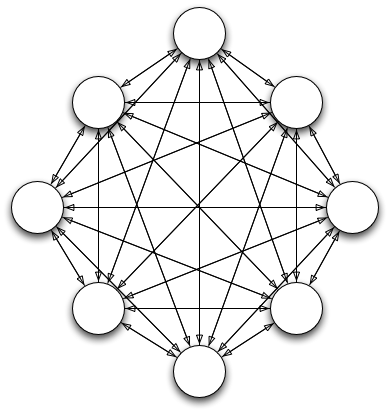
\includegraphics[width=0.5\textwidth]{imgs/hopfield.png} 
    \caption{A blueprint of a Hopfield nets with 8 binary units. The units are connected with symmetric undirected connections \cite{hopfImg}.}
    % http://blogs.cetis.org.uk/wilbert/2009/04/07/ims-qti-and-the-economics-of-interoperability/
	\label{fig:hopfiled}
\end{figure}


In contrast to feed-forward networks in Hopfield nets, there is no clearly defined bottom layer and order of the layers, thus the updates can be performed in two different way :
\begin{itemize}
\item Asynchronous: One unit is updated at a time. The units are either chosen randomly or in a predefined order
\item Synchronous: All units are updated at the same time (based on the previous states of all units)
\end{itemize}

Similar to energy based models each state $z = (s_1, ... , s_n)$ can be described by an energy, which for Hopfield nets the energy of a state is defined as  
\[
E(z) = - \frac{1}{2} \sum w_{ij} s_i s_j + \sum b_i s_i .
\]


By introducing recurrent connections, the network can be trained to store information.
Indeed, with each (asynchronous) update step the energy is thus guaranteed to stay the same or lower in value.
And thus the network will converge to a local minimum of the energy function, similar to a stable equilibrium state, where it can not escape from. 
Such a state can be called mode or attractor state.
Hopfield nets can be trained as associative memory, where each stored pattern corresponds to such an attractor state.

The training rule for associative memory is a local Hebbian rule, i.e. for an update they only use information of neurons on either side of a connection:
\[
w_{ij} = \frac{1}{n} \sum_{patterns} s_{i} s_{j}
\]

Such Hopfields net can consequently perform pattern completion by reaching a low energy state, but it can also end in a spurious state, an attractor state/local energy minimum, which was not presented as a training data.


\subsubsection{Boltzmann Machines} \label{c:bms}

Boltzmann machines try to improve Hopfield nets by replacing the deterministic update rule with a stochastic one.
This allows a more stochastic exploration of the network states due to probabilistic escaping of minima states \cite{ackley1985learning} \cite{Goodfellow-et-al-2016-Book}.

\paragraph{Model} \label{c:bmmodel}

Similar to a Hopfield net the units $s_i$ in a Boltzmann machine are binary as well and can have the value $s_i = 1$ or $s_i = 0$. 
A further similarity are bidirectional, symmetric weights without any self connections, and an equivalent energy function:
\[
	E(z) = - \frac{1}{2} \sum w_{ij} s_i s_j + \sum b_i s_i .
\]
This allows the interpretation of a Boltzmann machine as an energy based model with the probability distribution defined by the energy function $E$ and its parameters $\textbf{w}$.

A Boltzmann machine is an energy based model with the probability distribution defined by the Energy.
Thus each state $\textbf{z}$ can be assigned a Energy which is directly indicates the probability of the state $P(\textbf{z}) \propto -E(\textbf{z})$:
\[
P(\textbf{z}) = - \frac{1}{Z} \exp^{-E(\textbf{z})} 
\]

A unit is updated probabilistically given the states of its neighbour units:
\[
p_{on}(s_i) = \sigma( \sum s_j w_{ij} + b_i ), 
\]
where $\sigma$ is the sigmoid-function.

An update step can be seen as a Gibbs sampling step from the distribution defined by $E$.
Running a certain number of consecutive update steps probabilistically drives the network to a low energy or equilibrium state.


\begin{figure}
	\centering
    	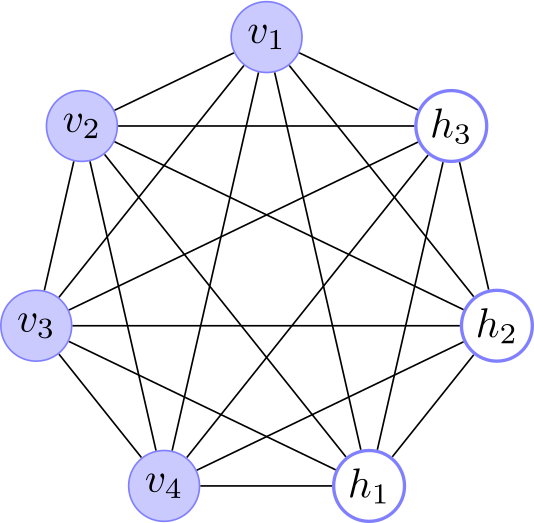
\includegraphics[width=0.5\textwidth]{imgs/bm.png} 
    \caption{A Boltzmann machine with 7 units. In contrast to a Hopfield nets, units are divided into visible and hidden/ unobserved units with stochastic activations \cite{boltzImg}.}
    % http://gorayni.blogspot.de/
	\label{fig:bm}
\end{figure}

In contrast to Hopfield nets where each unit of the network is represented by a element a data sample, in Boltzmann machines latent variables are introduced to increase the capacity of the network.
The units are thus divided into observable visible units and unobservable hidden/latent units (see Fig \ref{fig:bm}).
With hidden units a Boltzmann machine becomes a universal approximation probability mass functions over discrete variables.


\paragraph{Learning Rule} \label{c:cd}

The goal for training a Boltzmann machine is to get a probability distribution, which is similar to the distribution which generated the training data, the so-called data distribution.
Thus the objective for a Boltzmann machine is to assign a high probability to its training data (while assigning a low probability data not drawn from the data distribution) \cite{ackley1985learning} \cite{hinton2002training} \cite{Woodford2002} \cite{Bengio2009}.
By using gradient descent we will adapt the parameters/ weights of the Boltzmann machine in a directions which assigns trainings samples $\textbf{x}$ a high probability:
\[
w_{ij} = w_{ij} - \mu \Delta w_{ij},
\]
where
\[
\Delta w_{ij} = \frac{\partial P(\textbf{x})}{\partial w_ij}.
\]

By using the logarithm of the probability function $\frac{\partial P(\textbf{x})}{\partial w_{ij}}$ can be rewritten as
\[
\frac{\partial P(\textbf{x})}{\partial w_{ij}} = \frac{\partial Z}{\partial w_{ij}} - \frac{1}{K} \sum_{i=1}^K \frac{\partial \log E(\textbf{x}_i)}{\partial w_{ij}} =  \frac{\partial Z}{\partial w_{ij}} - \Big \langle \frac{\partial \log E(\textbf{x})}{\partial w_{ij}} \Big \rangle_{\text{data}}.
\]    

The derivation of the partition function $Z$ by $w_{ij}$ can be restated as
\[
 \frac{\partial Z}{\partial w_{ij}} = \int p(\textbf{x}) \frac{\partial \log E(\textbf{x})}{\partial w_{ij}} dx = \Big \langle \frac{\partial \log E(\textbf{x})}{\partial w_{ij}} \Big \rangle_{\text{model}}.
\]

Thus the update rule is now given as
\[
\frac{\partial P(\textbf{x})}{\partial w_ij} =  \Big \langle \frac{\partial \log E(\textbf{x})}{\partial w_{ij}} \Big \rangle_{\text{model}} - \Big \langle \frac{\partial \log E(\textbf{x})}{\partial w_{ij}} \Big \rangle_{\text{data}}
\]
The derivation of $\log E$ after a weight $w_{ij}$
\[
\frac{\partial \log E(\textbf{x})}{\partial w_{ij}} = s_i s_j
\]

gives the quite simple update rule called contrastive divergence (CD)
\[
w_{ij}= w_{ij} + \mu ( \langle s_i s_j \rangle_{\text{data}} - \langle s_i s_j \rangle_{\text{model}} ) ,
\]
where $\langle s_i s_j \rangle_{\text{data}}$ are the expected activations from the data distribution and  $ \langle s_i s_j \rangle_{\text{model}}$ are the expected activations from the model distribution.
The most common way to get the data and model distribution is to perform consecutive Gibbs update steps until an equilibrium distribution is reached, with either training data clamped or no data clamped to visible units.

Here $\langle s_i s_j \rangle_{\text{data}}$ is referred to as the positive phase and $ \langle s_i s_j \rangle_{\text{model}}$ as negative phase.
A simple interpretation of the update rule is a shift of the weights away from the model distribution towards the data distribution.

\subsubsection{RBMs} \label{c:rbms}

To perform such an update, samples from the model distribution are needed. 
To get those samples, the Boltzmann machine has to reach an equilibrium distribution. 
This can be quite computationally expensive and there is no guarantee to tell when the equilibrium distribution is reached.
Thus potentially infinite sampling steps have to be performed.

To evade the problem, a simple solution is to make the hidden units not dependent on each other (and the visible not dependent on each other), so all hidden units can be sampled independent and parallel of each other.
Thus a Boltzmann machine with two bipartite layers is called restricted Boltzmann machine (RBM) (see Fig. \ref{fig:rbm}) \cite{smolensky1986information}.

Sampling the hidden units $\textbf{h}$ given the visible units $\textbf{v}$ is called a \textit{upward pass} and sampling the visible units $\textbf{v}$ given the hidden units $\textbf{h}$ is called a \textit{downward pass}.

In this case the probability of data sample $\textbf{x}$ can be expressed using the free energy $F(\textbf{v})$ over its visible activations $\textbf{v}$ \cite{hinton2010practical}\cite{Fischer2014}:
\[
p(\textbf{x}) =  p(\textbf{v}) = \sum_{\textbf{h}} \exp^{-E(\textbf{v},\textbf{h})} = \exp^{-F(\textbf{v})},
\]
where the free energy can also be expressed as
\[
F(\textbf{v}) = - \sum x_i b_i - \sum \log(1 + \exp^{x_i})  .
\]

\begin{figure}
	\centering
    	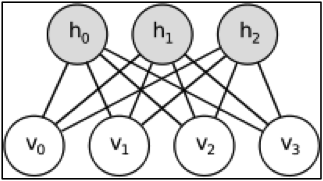
\includegraphics[width=0.5\textwidth]{imgs/rbm.png} 
    \caption{A restricted Boltzmann machine is special kind of Boltzmann machine with no lateral connections in the hidden and visible layer. This eases sampling, since the visible are only dependent on the hidden units and the hidden units only on the visible units \cite{rbmImg}.}
    % http://www.todaysoftmag.com/article/747/restricted-boltzmann-machines
	\label{fig:rbm}
\end{figure}

\paragraph{CD-k Training} \label{c:cdk}

The simplified structure of an RBM enables faster weight updates. 
Hinton showed empirically that this training procedure can be further improved by running only a limited number of Gibbs sampling steps to approximate the model distribution \cite{hinton2002training}.

The gradient calculated with this approximation can be seen as "good enough" to perform updates, which drive the underlying distribution towards the data distribution.

Thus given a data sample $\textbf{x}$ an CD-k update is computed as follows:
\begin{enumerate}
\item Perform one upward pass given $\textbf{v}_0=\textbf{x}$ to get $\textbf{h}_0$.
\item Perform k alternating downward and upward passes to get $\textbf{v}_k$ and $\textbf{h}_k$.
\item Update $w_{ij} = w_{ij} + ( (s_i s_j)_0 - (s_i s_j)_k ) $ 
\end{enumerate} 

\begin{figure}
	\centering
    	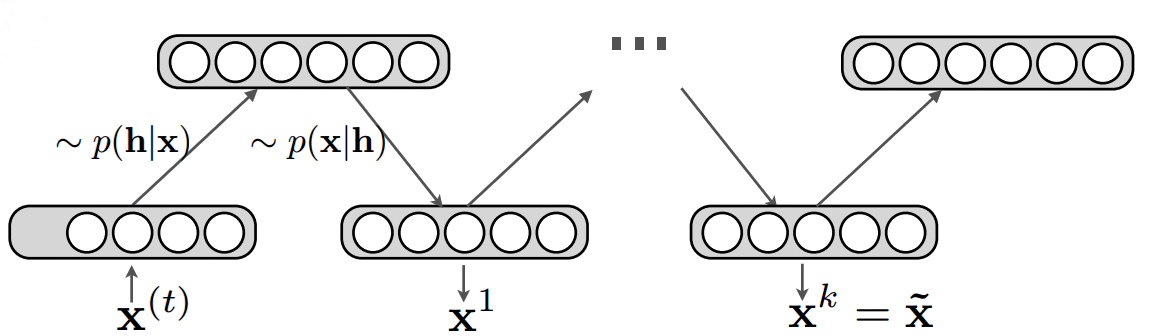
\includegraphics[width=0.8\textwidth]{imgs/cd.png} 
    \caption{A temporal unrolling of the contrastive divergence algorithm with $k$ sampling step. The hidden units and the visible units are alternatingly sampled conditioned on the current state of the other \cite{cdImg}.}
    % http://recognize-speech.com/acoustic-model/knn/training-neural-networks
	\label{fig:cd}
\end{figure}

In Figure \ref{fig:cd} the sampling steps are visualized by unrolling the RBM as a directed model.

\paragraph{Persistent CD} \label{c:pcd}

, proposed by Tieleman, does not initialize the Boltzmann machine new each time a new sample is drawn, but uses the activations of previous runs instead \cite{tieleman2008training}. An intuition why it sometimes shows better performance could be that the previous activations are already closer to an energetic minimum, so that fewer step are required to get an good estimate of the model distribution. 


\subsubsection{Deep Belief Networks} \label{c:dbns}

A deep belief network (DBN) is a generative graphical model, or alternatively a type of deep neural network, composed of multiple layers of latent variables (hidden units), with connections between consecutive layers, but with no connections within layer \cite{hinton2006fast} \cite{hinton2009deep} \cite{Goodfellow-et-al-2016-Book}.

A deep belief network can be built up by stacking up RBMs.
This does not only enable unsupervised training of a deep belief net, but also improves the conditional distribution of the bottom RBM (each time a RBM is added, it improves the prior over the hidden units with a better and more complex prior).

In a deep belief net the two top layers form a RBM with symmetric weights while the weight symmetry can be broken up between the lower layers to allow unsymmetrical weights.   

\paragraph{Training} \label{c:dbntraining}

Training of a DBN can be split up into greedily training simple RBMs on a cascade of stacked up RBMs (see Fig. \ref{fig:dbn}).
The training procedure can be formalized as:  
\begin{enumerate}
\item Train a new top RBM given the transformed data from the bottom layers
\item After training one RBM, transform the training data by sampling the hidden layer activations of the top RBM
\end{enumerate}

After training, the DBN still has symmetric weights. 

\begin{figure}
	\centering
    	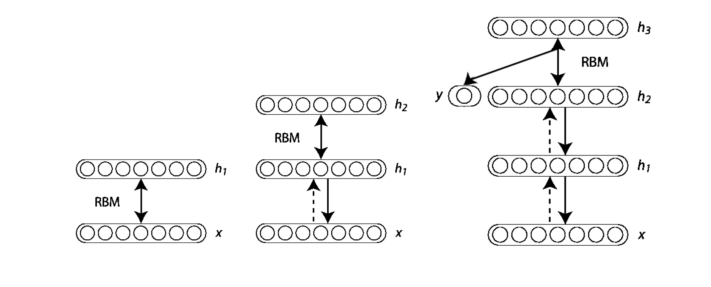
\includegraphics[width=0.8\textwidth]{imgs/dbn_stacking.png} 
    \caption{Building up a deep belief network, by training RBMs greedily and stacking them up on top of each other. At first only one RBM is trained. On top of the first RBM the next RBM is trained. This can procedure can be performed for an arbitrary number of repetitions. In the top layer "association" RBM the label information $y$ can be in-cooperated as well \cite{cdImg}.}
    % http://recognize-speech.com/acoustic-model/knn/training-neural-networks
	\label{fig:dbn}
\end{figure}

\paragraph{Fine-tuning} \label{c:dbnfinetuning}

After greedily training the DBN, the bidirectional connections can be split up and fine tuned to a certain task.
In general there are two most used fine-tuning algorithms, the wake-sleep algorithm for data generation and the backprop algorithm for classification. 

In the wake-sleep algorithm the symmetric weights are split up into bottom-up and top-down weights and are fine-tuned individually \cite{hinton1995wake}
\begin{enumerate}
\item Do a stochastic forward pass, and for each layer adjust the top-down weights, to better reconstruct the activations in the layer below.
\item Perform sampling steps in the top level RBM and adjust the weights with CD.
\item Do a stochastic backward pass, and for each layer adjust the bottom-up weights, to better reconstruct the activations in the layer above.
\end{enumerate}

Another way to fine-tune the weights for classification given labels and an error function, is to perform back propagation to further fine tune the bottom-up weights (while the top-down weights are usually discarded). 
One interpretation of this is to see a DBN as a pre-trained ANN.

\subsection{Spiking neural networks} \label{c:snns}

While all the previous presented models did run at discrete time steps, the next models are designed to run contentiously which makes them more similar to natural neurons and neural networks \cite{maass1997networks}. 

\subsubsection{Neuron Models} \label{c:snnneurons}

Similar to the activation function in ANNs, in SNNs there are also different models describing how neurons process input.
Most neuron models describe the development of a neuron's membrane potential over time.
Therefore the models commonly have a resting potential, which describes the membrane potential a rest without any external influences. 
Most models also have a way to model external input from incoming spikes and an internal leakage pulling the membrane potential back to its resting potential. 
If a "pseudo" threshold is exceeded usually a spike is emitted and the neuron reaches a refractory phase for some time.

\paragraph{LIF} \label{c:lif}

The leaky integrate and fire (LIF) neuron is a neuron model, which phenomenological describes the membrane potential at the soma \cite{abbott1999lapicque}\cite{gerstner2014neuronal}\cite{Petrovici2016}. 
It is one of the simplest and thus computationally most efficient, most important and popular spiking neuron models.  

\begin{figure}
	\centering
    	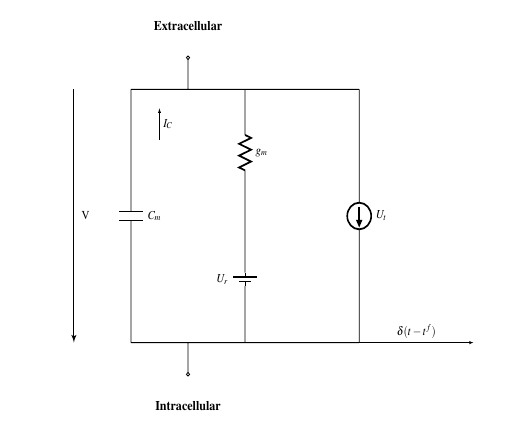
\includegraphics[width=0.6\textwidth]{imgs/lif.png} 
    \caption{A LIF neuron as an electrical circuit. The capacitor $C_m$ corresponds to the potential at the membrane, $g_l$ the leakage potential and $E_l$ the resting potential. If the membrane potential is greater than $U_t$ a spike $\delta$ is emitted \cite{heikoMA}.}
    % Heiko
	\label{fig:lif}
\end{figure}

By discarding the different forms/shapes of the action potentials and reducing it the uniform spike events, the information in condensed to the precise spike times.
The model, described by linear equations, models the membrane potential integration due to spike input currents with a capacitor and introduces a leaky current with a resistor. 
The model can be represented by a circuit of a single capacitor and a resistor with a battery (see Fig. \ref{fig:lif}):
\[
C_m \frac{\partial u}{\partial t} = g_l ( E_l - u(t) ) + I^{syn} + I^{ext} , 
\]
where $C_m$ is the membrane capacitance, $g_l$ is the leak conductance, $E_l$ the resting potential and the input current $I = I^{syn} + I^{ext}$ is divided into a static external input $I^{ext}$ and a synaptic input $I^{syn}$.   

If the membrane potentiality exceeds a threshold $\theta$ a spike $s$ is emitted and the membrane potential is instantaneously pulled back to it's reset potential $u_{reset}$ and kept at this potential for its refractory period $t_{ref}$.
\[
u(t_{s} < t \le t_{s} + t_{ref}) = u_{reset}.
\]

The emitted spikes are modelled as a spike train $\rho$ using only the precise spike times:
\[
\rho(t) = \sum_{\text{spikes } s} \delta(t-t_s),
\] 
where $\delta$ is the Dirac delta function.

Due to its simplifications the LIF model can not capture some natural observed behaviour such as bursting or adaptation (see Fig. \ref{fig:neuronbe}). 

\begin{figure}
	\centering
	\begin{subfigure}[t]{.32\textwidth}
	 	\centering
  		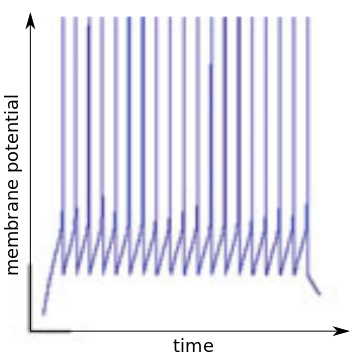
\includegraphics[width=.9\linewidth]{imgs/lif_bad1.png}
  		\caption{Constant tonic firing}
	\end{subfigure}
	\begin{subfigure}[t]{.32\textwidth}
	 	\centering
  		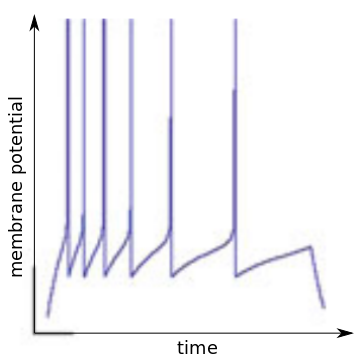
\includegraphics[width=.9\linewidth]{imgs/lif_bad2.png}
  		\caption{Frequency adaptation}
	\end{subfigure}
	\begin{subfigure}[t]{.32\textwidth}
	 	\centering
  		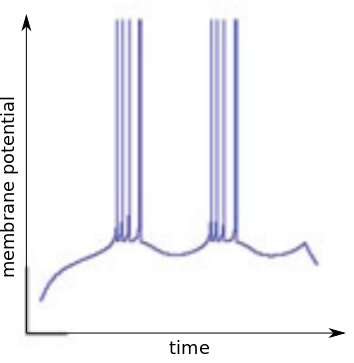
\includegraphics[width=.9\linewidth]{imgs/lif_bad3.png}
  		\caption{Delayed regular bursting}
	\end{subfigure}
    \caption{Different firing behaviour observed in the Brain. In (a) a neuron shows constant tonic firing, while in (b) the neuron shows frequency adaptation and in (c) the neurons shows delayed regular bursting \cite{gerstner2014neuronal}.}
	\label{fig:neuronbe}
\end{figure}



\paragraph{Hodgkin-Huxley} \label{c:hodghux}

The Hodgkin-Huxley model tries to improve some of the limitations of the LIF model, by explicitly allowing to model different ion channels \cite{Hodgkin1952}\cite{gerstner2014neuronal}. 

The first model described by Hodgkin-Huxley introduced three different ion channels, namely sodium, potassium and a leak current of $\text{CL}^{-}$ ions, which they discovered in their experiments on axon of a squid.
Each channel is described as a resistor with a battery (see Fig. \ref{fig:hogdehux}).
The Hodgkin-Huxley model with three ion channels can be described by the following equations :
\[
C_m \frac{\partial u}{\partial t} = g_{Na} m^3 h (E_{Na} - u(t)) + g_K n^4 (E_K - u(t)) + g_l (E_l - u(t)) + I,
\]

where the variables $h$, $m$, $n$  are described by :
\[
\begin{split}
	\frac{\partial h}{\partial t} = \alpha_h u(t) (1-h) - \beta_h u(t) * h , \\
	\frac{\partial m}{\partial t} = \alpha_m u(t) (1-m) - \beta_m u(t) * m , \\
	\frac{\partial n}{\partial t} = \alpha_n u(t) (1-n) - \beta_n u(t) * n ,
\end{split}
\]
with the rate constants $\alpha$, $\beta$ for each ion channel.

\begin{figure}
	\centering
    	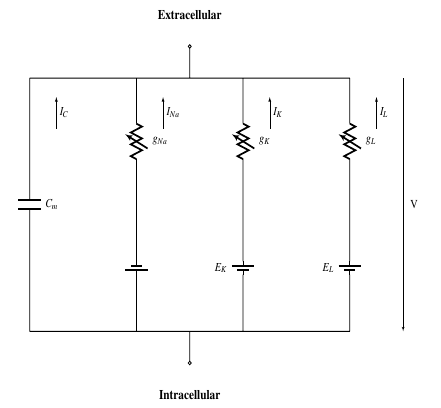
\includegraphics[width=0.6\textwidth]{imgs/hode_hux.png} 
    \caption{A Hodgkin-Huxley as an electrical circuit. The membrane potential corresponds to $C_m$, and the ion channels to $g_{Na}$, $g_{k}$, $g_{L}$ with their reversal potentials $E_{Na}$, $E_{}$, $E_{L}$ \cite{heikoMA}.}
    % Heiko
	\label{fig:hogdehux}
\end{figure}

This model can be extended/generalized to model more than three ion channels with their dynamics, to better match the characteristics/biophysics of different neurons in the brain:
\[
C_m \frac{\partial u}{\partial t} = \sum_{k \in K} g_k m^{p_k} h^{q_k} (E_k - u(t)) + I,
\]
with an arbitrary number of ion channels $K$.

While this allows the model to predict and simulate various effects observed in the brain, like frequency adaptation, with high accuracy, the Hodgkin-Huxley model is more computationally expensive.

\paragraph{Activity in a network} \label{c:poissonspikes}

One way to introduce activity into a spiking neural network is to use a Poisson spike generator \cite{Heeger2000}.
A Poisson spike generator produces stochastic firing according to a Poisson point process.
The firing rate $\lambda$ or rate function $\lambda(t)$ determines the dynamics of the homogeneous or inhomogeneous Poisson process respectively and thus of the spike times.   

The probability of a emitted spike in an time interval $\delta t$ is given by: 
\[
P_{spike}({t , t+ \delta t}) = \lambda(t) \delta t,
\]
where the occurrence of a spike is independent on previous spikes. 

Since the spikes can be formalized as a Poisson process, the expected number of spikes for an time interval $\delta t$ is given by :
\[
\langle  P_{spike}({t , t+ \delta t}) \rangle = \int_t^{t + \delta t} \lambda(t) dt.
\]


\subsubsection{Synapses} \label{c:synapses}

While synapses in ANNs are simply multiplying an incoming input with their weights, for SNNs there are different models which add additional dynamics to closer model naturally observed behaviour. 

The behaviour of the synapses are described by modelling the synaptic input $f^{syn}$. A basic model of how the influence of synapses can be described as follows \cite{Petrovici2016}:
\[
f^{syn}(t) = \sum_{\text{synapses } k } \sum_{\text{spikes } s} w_k \varepsilon(t - t_s),
\]
where $\varepsilon$ is a function describing the spike shape of the post synaptic potential (PSP).
Different shapes will discussed in the paragraph \textit{Kernel functions} \ref{c:pspkernel}.

\paragraph{Current-based synaptic interaction} \label{c:cuba}
One synapse type models the input current of neuron $I^{syn}$ directly as the synaptic input $f^{syn}$. This is a logical implementation for LIF neurons since they directly model the potential at the soma and don't consider most of the membrane dynamics in the dendrites. 
Thus the synaptic input current is given as a linear summation of the post synaptic potentials with temporal effects:
\[
I^{syn}(t) = \sum_{\text{synapses } k } \sum_{\text{spikes } s} w_k \epsilon(t - t_s),
\]
where $\epsilon$ is a kernel describing the explicit shape of a post synaptic spike.

\paragraph{Conductance-based synaptic interaction} \label{c:coba}
Conductance-based synapse models describe the synaptic dynamics more closely to its natural counterpart. They consider the conductance changes of incoming spikes, which push the conductance locally towards the reversal potential of the specific ion type. 

In this case the synaptic input $f^{syn} $can be seen as a change in the synaptic membrane conductance $g^{syn}$ :
\[
g_x^{syn} = \sum_{\text{synapses } k } \sum_{\text{spikes } s} w_k \epsilon(t - t_s) \text{ ,      } x \in \{e, i\}.
\]

Thus the synaptic input current $I^{syn}$ can now be described using the membrane conductance by applying Ohm's law:
\[
I^{syn}(t) = g_e^{syn} (E_e^{rev} - u(t)) + g_i^{syn} (E_i^{rev} - u(t)),
\]
where $E_e^{rev}$ and $E_i^{rev}$ is the excitatory and inhibitory reversal potential of the membrane, which can be e.g. chosen as $E_{Na}$ and $E_{K}$ respectively.  

\subparagraph{High conductance state} \label{c:hcs}
One interesting property of conductance based neurons is, that they can reach a so-called high conductance state (HCS) \cite{Petrovici2016}. Such a state is defined by a high total membrane conductance 
\[
g^{tot} = g_l + \sum_{\text{synapses } k} g_k^{syn},
\]
with 
\[
\sum_{\text{synapses } k} g_k^{syn} =: g^{syn} >> g_l .
\]
Such a state can be reached by a lot of incoming synaptic firing. e.g. high frequency Poisson noise from other neurons. 

The HCS is especially interesting, because the dynamics of the membrane potential can be described by a Gaussian process called Ornstein–Uhlenbeck process, with a mean primarily determined by the effective synaptic input (with the noise) and the variance by the total membrane conductance (see Fig. \ref{fig:ornuhl}).
In addition Petrovici showed, that in such a state the time the neuron needs to get from its resting potential to a value given by Ornstein–Uhlenbeck process can basically be neglected (see Fig. \ref{fig:hcs}).
This will show further application as a stochastically firing neuron model used for neural sampling  in Chapter \ref{c:snnsampling}.

\begin{figure}
	\centering
    	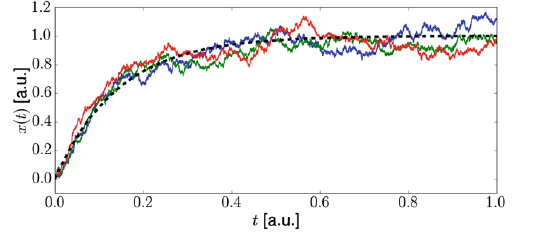
\includegraphics[width=0.6\textwidth]{imgs/orn_uhl_process.png} 
    \caption{Three samples of Ornstein–Uhlenbeck processes. This can be seen as the membrane potential of neurons in a high conductance state (in comparison to the black doted line can be seen as a neuron without noisy input) \cite{Petrovici2016}.}
    % Petrovici
	\label{fig:ornuhl}
\end{figure}


\begin{figure}
	\centering
    	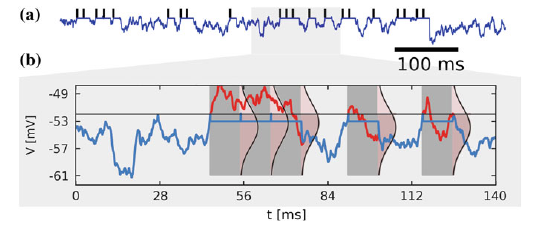
\includegraphics[width=0.6\textwidth]{imgs/hcs.png} 
    \caption{A membrane potential trajectory of a neuron in a high conductance state. (a) The spike train and the membrane potential. (b) The blue curve represents the actual membrane potential with refractory periods after each spike, while the red curve represents a membrane potential without a firing threshold. It is apparent, that the blue curve returns the the hypothetical red potential without a "return from rest" time  \cite{Petrovici2016}. }
    % Petrovici
	\label{fig:hcs}
\end{figure}


\paragraph{Kernel function} \label{c:pspkernel}

Next to the synaptic models, the kernel function $\epsilon$ has probably the most important part in modelling the synaptic input current $I^{syn}$. 
The kernel describes the explicit shape of the post synaptic potential over time and thus the influence it has on the membrane potential.
There have been several different kernel proposed, whereof some of the most important are:
\begin{itemize}
\item Rectangular-shaped: \[\epsilon(t) \propto  \begin{cases} 1, & \text{ if } t_{s} < t \le t_{s} + t_{ref} \\ 0, & \text{ otherwise } \end{cases} \]
\item Exponential-shaped: $\epsilon(t) \propto t \exp(- \frac{t}{\tau_syn})$
\item Alpha-shaped: $\epsilon(t) \propto \exp(- \frac{t}{\tau_syn})$
\end{itemize}

These are also visualized in Figure \ref{fig:pspkernels}.

\begin{figure}
	\centering
    	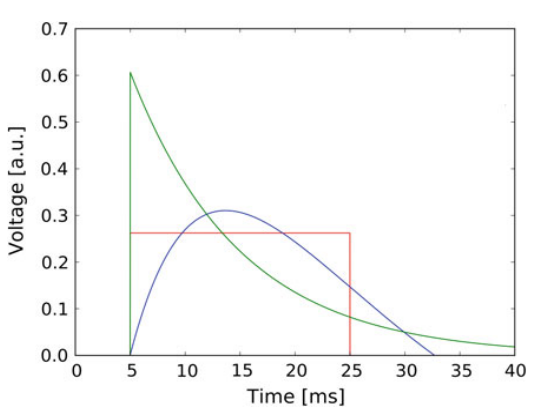
\includegraphics[width=0.6\textwidth]{imgs/psp_kernel.png} 
    \caption{Three different PSP kernels. The green one has an alpha-shape, the blue one is exponential shaped and the red one is rectangular \cite{Petrovici2016}. }
    % Petrovici
	\label{fig:pspkernels}
\end{figure}

\subsubsection{Neural Coding} \label{c:neuralcoding}

Spikes are the primary way of information transmission in the brain.
In neural networks this information can be encoded in different ways.
We will present three encoding mechanisms, which were observed in the brain, rate coding, temporal coding and population coding \cite{Meftah2013}.

In the \textit{rate coding} scheme the information is purely contained in the spike frequency/ firing rate of a neuron.
In contrast to rate coding, in \textit{temporal coding} the information is additionally transmitted via the different points in time at which the spikes are transmitted. 
Thus the information is carried in the exact spike timings.
\textit{Population coding} encodes information as the joint activity of several neurons in a population.  

In this thesis we use temporal or rate encoded input data, which is in the network represented as a population coded state over the joint activity of several neuron and is decoded in a rate-based manner. 

\subsubsection{Learning} \label{c:snnlearning}

Learning in the brain describes the generalized term, how information in the brain is stored (in contrast to task learning, memory adaptation is also considered learning).

Most models of learning algorithms in spiking neural networks build on changes in the synaptic weights/ strength between neurons to store information \cite{gerstner2014neuronal}.
To consider these changes as learning, they have to span over minutes to days or more, which is described by long term plasticity, e.g by LTP (long-term potentiation), LTD (long-term depression) or STDP (see Fig. \ref{fig:stdp}).
 
The models most commonly used are inspired on the research and discoveries of Hebb and the previously discussed Hebb principle (Chapter \ref{c:hebb}).

\paragraph{Spike time dependent plasticity} \label{c:stdp}

Spike time dependent plasticity (STDP), inspired by research on single neurons with artificially induced current, describes such a Hebbian learning algorithm.

Experiments indicated an increase of the synaptic weight if a post-synaptic spike occurred in strong temporal vicinity after a pre-synaptic spike and a decrease of the synaptic weight if a post-synaptic spike occurred in strong temporal vicinity before a pre-synaptic spike.
The further apart the spike times of the different neurons were, the weaker was the effect on the spike (see Fig. \ref{fig:stdp}).

Given the spike times of the pre- and post-synaptic neurons $t^{pre}$ and $t^{post}$, this leads to the following update rules \cite{gerstner2014neuronal}\cite{Sjostrom2010}
\[
\Delta w_{ij} = \sum_{f=1}^N \sum_{n=1}^N W(t^{post}_n - t^{pre}_f),
\]
with a common choice for the STDP function $W$
\[
W(x) =
\begin{cases}
A_+ \exp(\frac{-x}{\tau_+}) \quad \quad &\text{for  } x > 0,  \\
-A_- \exp(\frac{x}{\tau_-}) \quad \quad &\text{for  } x < 0,
\end{cases}
\]
given time constants $\tau_+$ and $\tau_-$ and the weight depend parameters $A_+$ and $A_-$.
     

\paragraph{Long-term potentiation} \label{c:ltp}
 
Long-term potentiation (LTP) can be interpreted as a STDP variant with only the positive part of the STDP function
\[
W(x) =  A_+ \exp(\frac{-x}{\tau_+}).
\]

This leads to a purely positive increase of weights (see Fig. \ref{fig:stdp}).

\paragraph{Long-term depression} \label{c:ldp}

Long-term depression (LTD) can be seen a the negative counterpart to LTP, with an STDP function
\[
W(x) =  -A_- \exp(\frac{x}{\tau_-}).
\]

This leads to a purely negative decrease of weights (see Fig. \ref{fig:stdp}).

\begin{figure}
	\centering
    	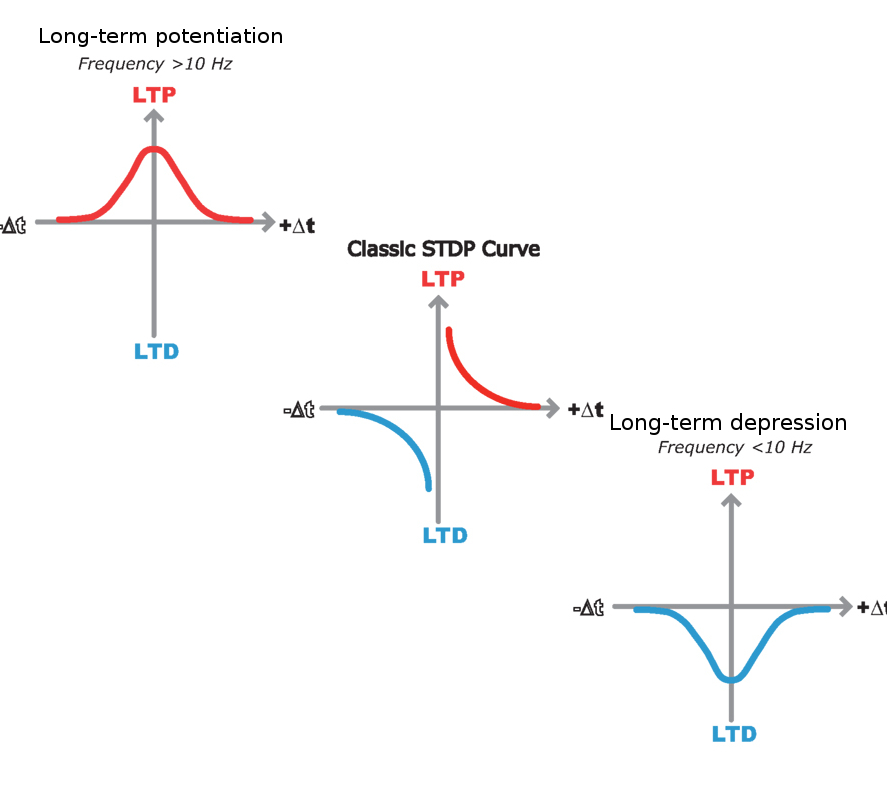
\includegraphics[width=0.6\textwidth]{imgs/stdp_curves.jpg} 
    \caption{Different STDP curves observed in the Brain. The first curve shows only long term potentiation. The middle one shows a variant of the classic STDP Curve and the last one shows purely long term depression \cite{Buchanan2010}.}
	\label{fig:stdp}
\end{figure}
\chapter{Related Work} \label{c:relwork}

In this section we present recent work related to convolutional RBMs, which have already been proposed in discrete time.
We further show recent approaches for sampling and implementing Boltzmann machines in spiking neural networks.

\section{Convolutional RBM} \label{c:convrbm}

The convolutional RBM (cRBM) was invented more or less at the same time by Desjardins et al., Lee et al. and Norouzi et al. in 2008/2009 \cite{desjardins2008empirical}\cite{lee2009convolutional}\cite{norouzi2009stacks}. 
In similarity to CNNs it can be seen as the adaptation of an energy-based models to compositional data.
Describing images in terms of spatially local features needs fewer parameters, generalizes better and offers re-usability as identical local features can be extracted from different locations of an image.
Modelled after CNNs and unlike a normal RBM, the visible and hidden layer in the cRBM are connected in a convolutional manner (as described in Chapter \ref{c:cnns}) instead of being fully connected.


Propagating information up can be seen as the convolution with a filter matrix $W$ (see Fig \ref{fig:convrbmsub1}): 
\[
P(\textbf{h} | \textbf{v}) = \sigma((W * \textbf{v}) + \textbf{b}_{h}).
\]
The down propagation utilizes the flipped kernel $\tilde{W}$  (see Fig \ref{fig:convrbmsub2} \& \ref{fig:convrbmsub3} ):
\[
P(\textbf{v}| \textbf{h}) = \sigma((\tilde{W} * \textbf{h}) + b_v).
\]
Using the convolution operation the energy of the network can thus be rewritten as
\[
E(\textbf{h} , \textbf{v}) = \textbf{h}^\intercal(W * \textbf{v}) + \textbf{h}^\intercal \textbf{b}_{h} + \sum b v_i.
\]

%\begin{figure}
%	\centering
%	\begin{subfigure}[t]{.30\textwidth}
%  		\centering
%  		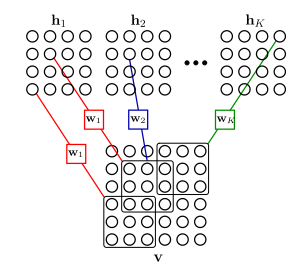
\includegraphics[width=.8\linewidth]{imgs/crbm1.png}
%  		\caption{A subfigure}
%  		\label{fig:sub1}
%	\end{subfigure}%
%	\begin{subfigure}[t]{.30\textwidth}
%  		\centering
%  		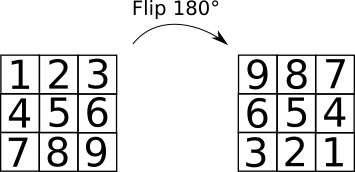
\includegraphics[width=.8\linewidth]{imgs/kernel_flip.png}
%  		\caption{A subfigure}
%  		\label{fig:sub2}
%	\end{subfigure}
%	\begin{subfigure}[t]{.30\textwidth}
%  		\centering
%  		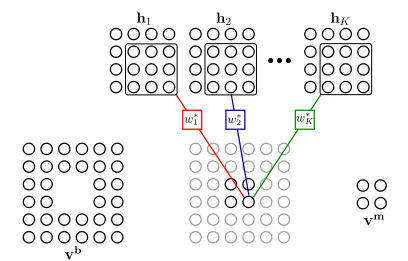
\includegraphics[width=.8\linewidth]{imgs/crbm2.png}
%  		\caption{A subfigure}
%  		\label{fig:sub3}
%	\end{subfigure}
%\end{figure}


\begin{figure}
	\centering
	\begin{subfigure}[t]{.30\textwidth}
  		\centering
  		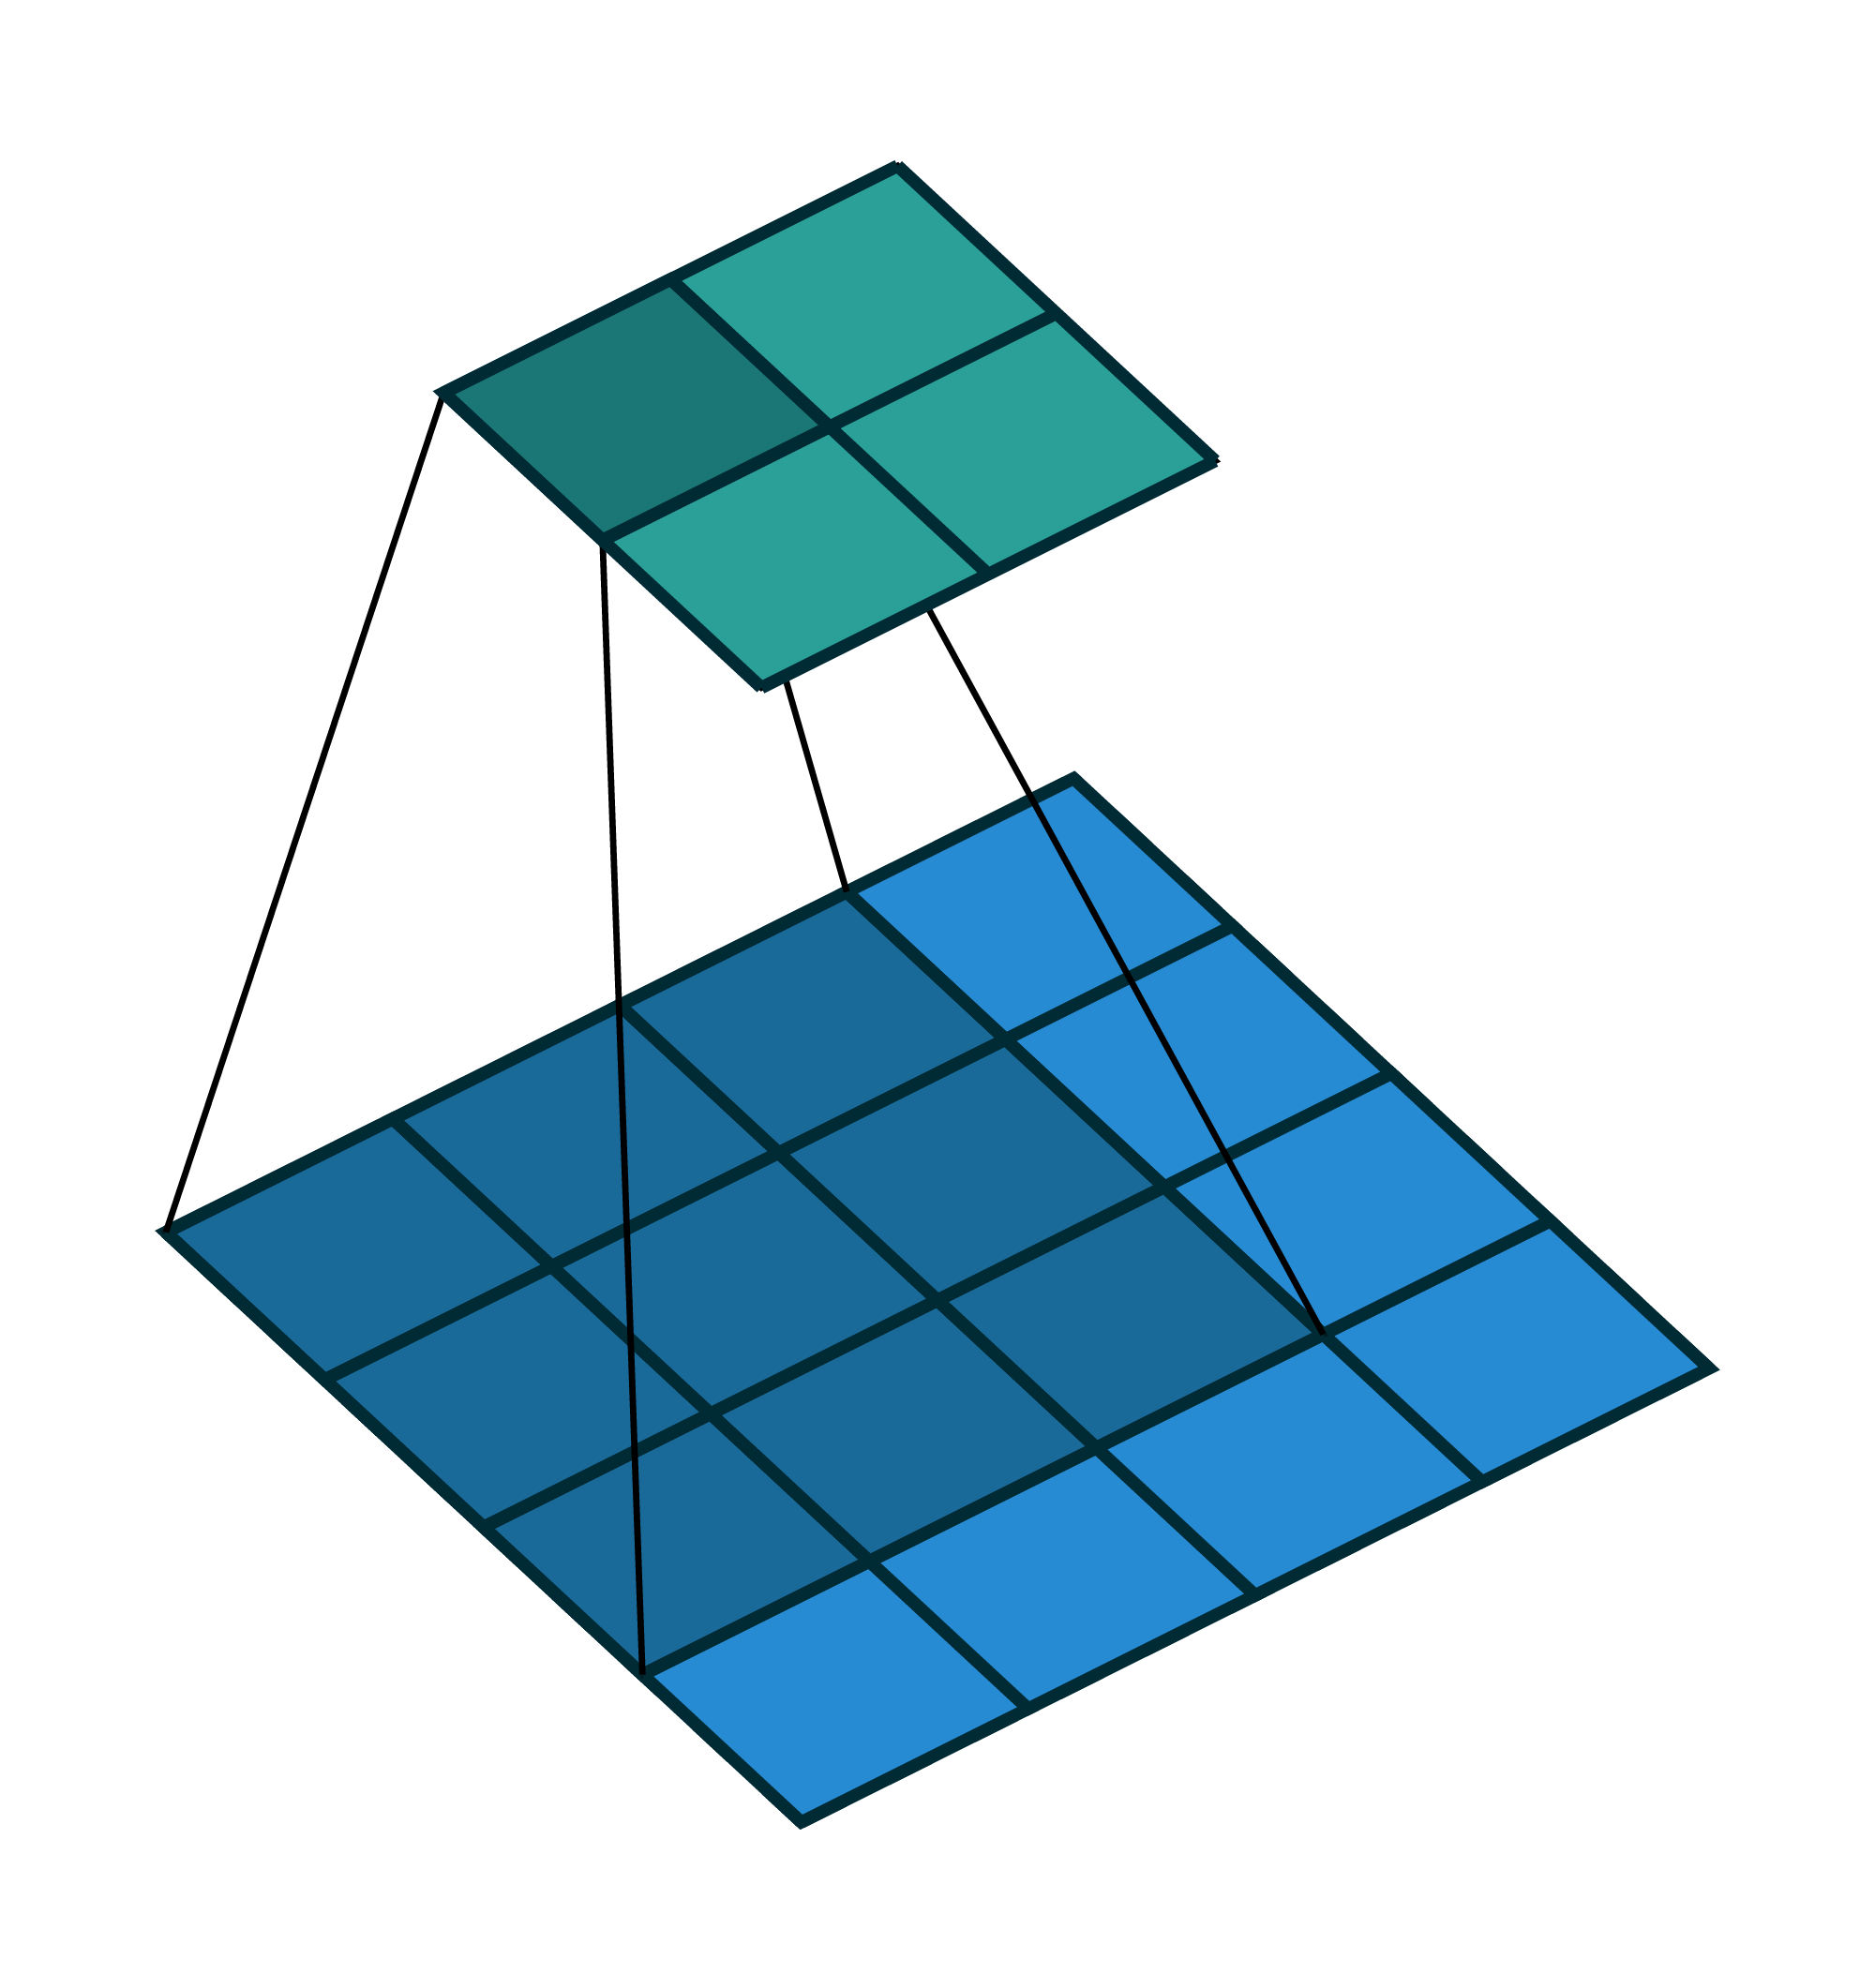
\includegraphics[width=.8\linewidth]{imgs/crbm_padding1.png}
  		\caption{The upward pass in the convolutional RBM}
  		\label{fig:convrbmsub1}
	\end{subfigure}%
	\begin{subfigure}[t]{.30\textwidth}
  		\centering
  		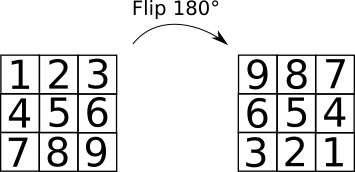
\includegraphics[width=.8\linewidth]{imgs/kernel_flip.png}
  		\caption{The 180\textdegree  flipped of the kernel matrix}
  		\label{fig:convrbmsub2}
	\end{subfigure}
	\begin{subfigure}[t]{.30\textwidth}
  		\centering
  		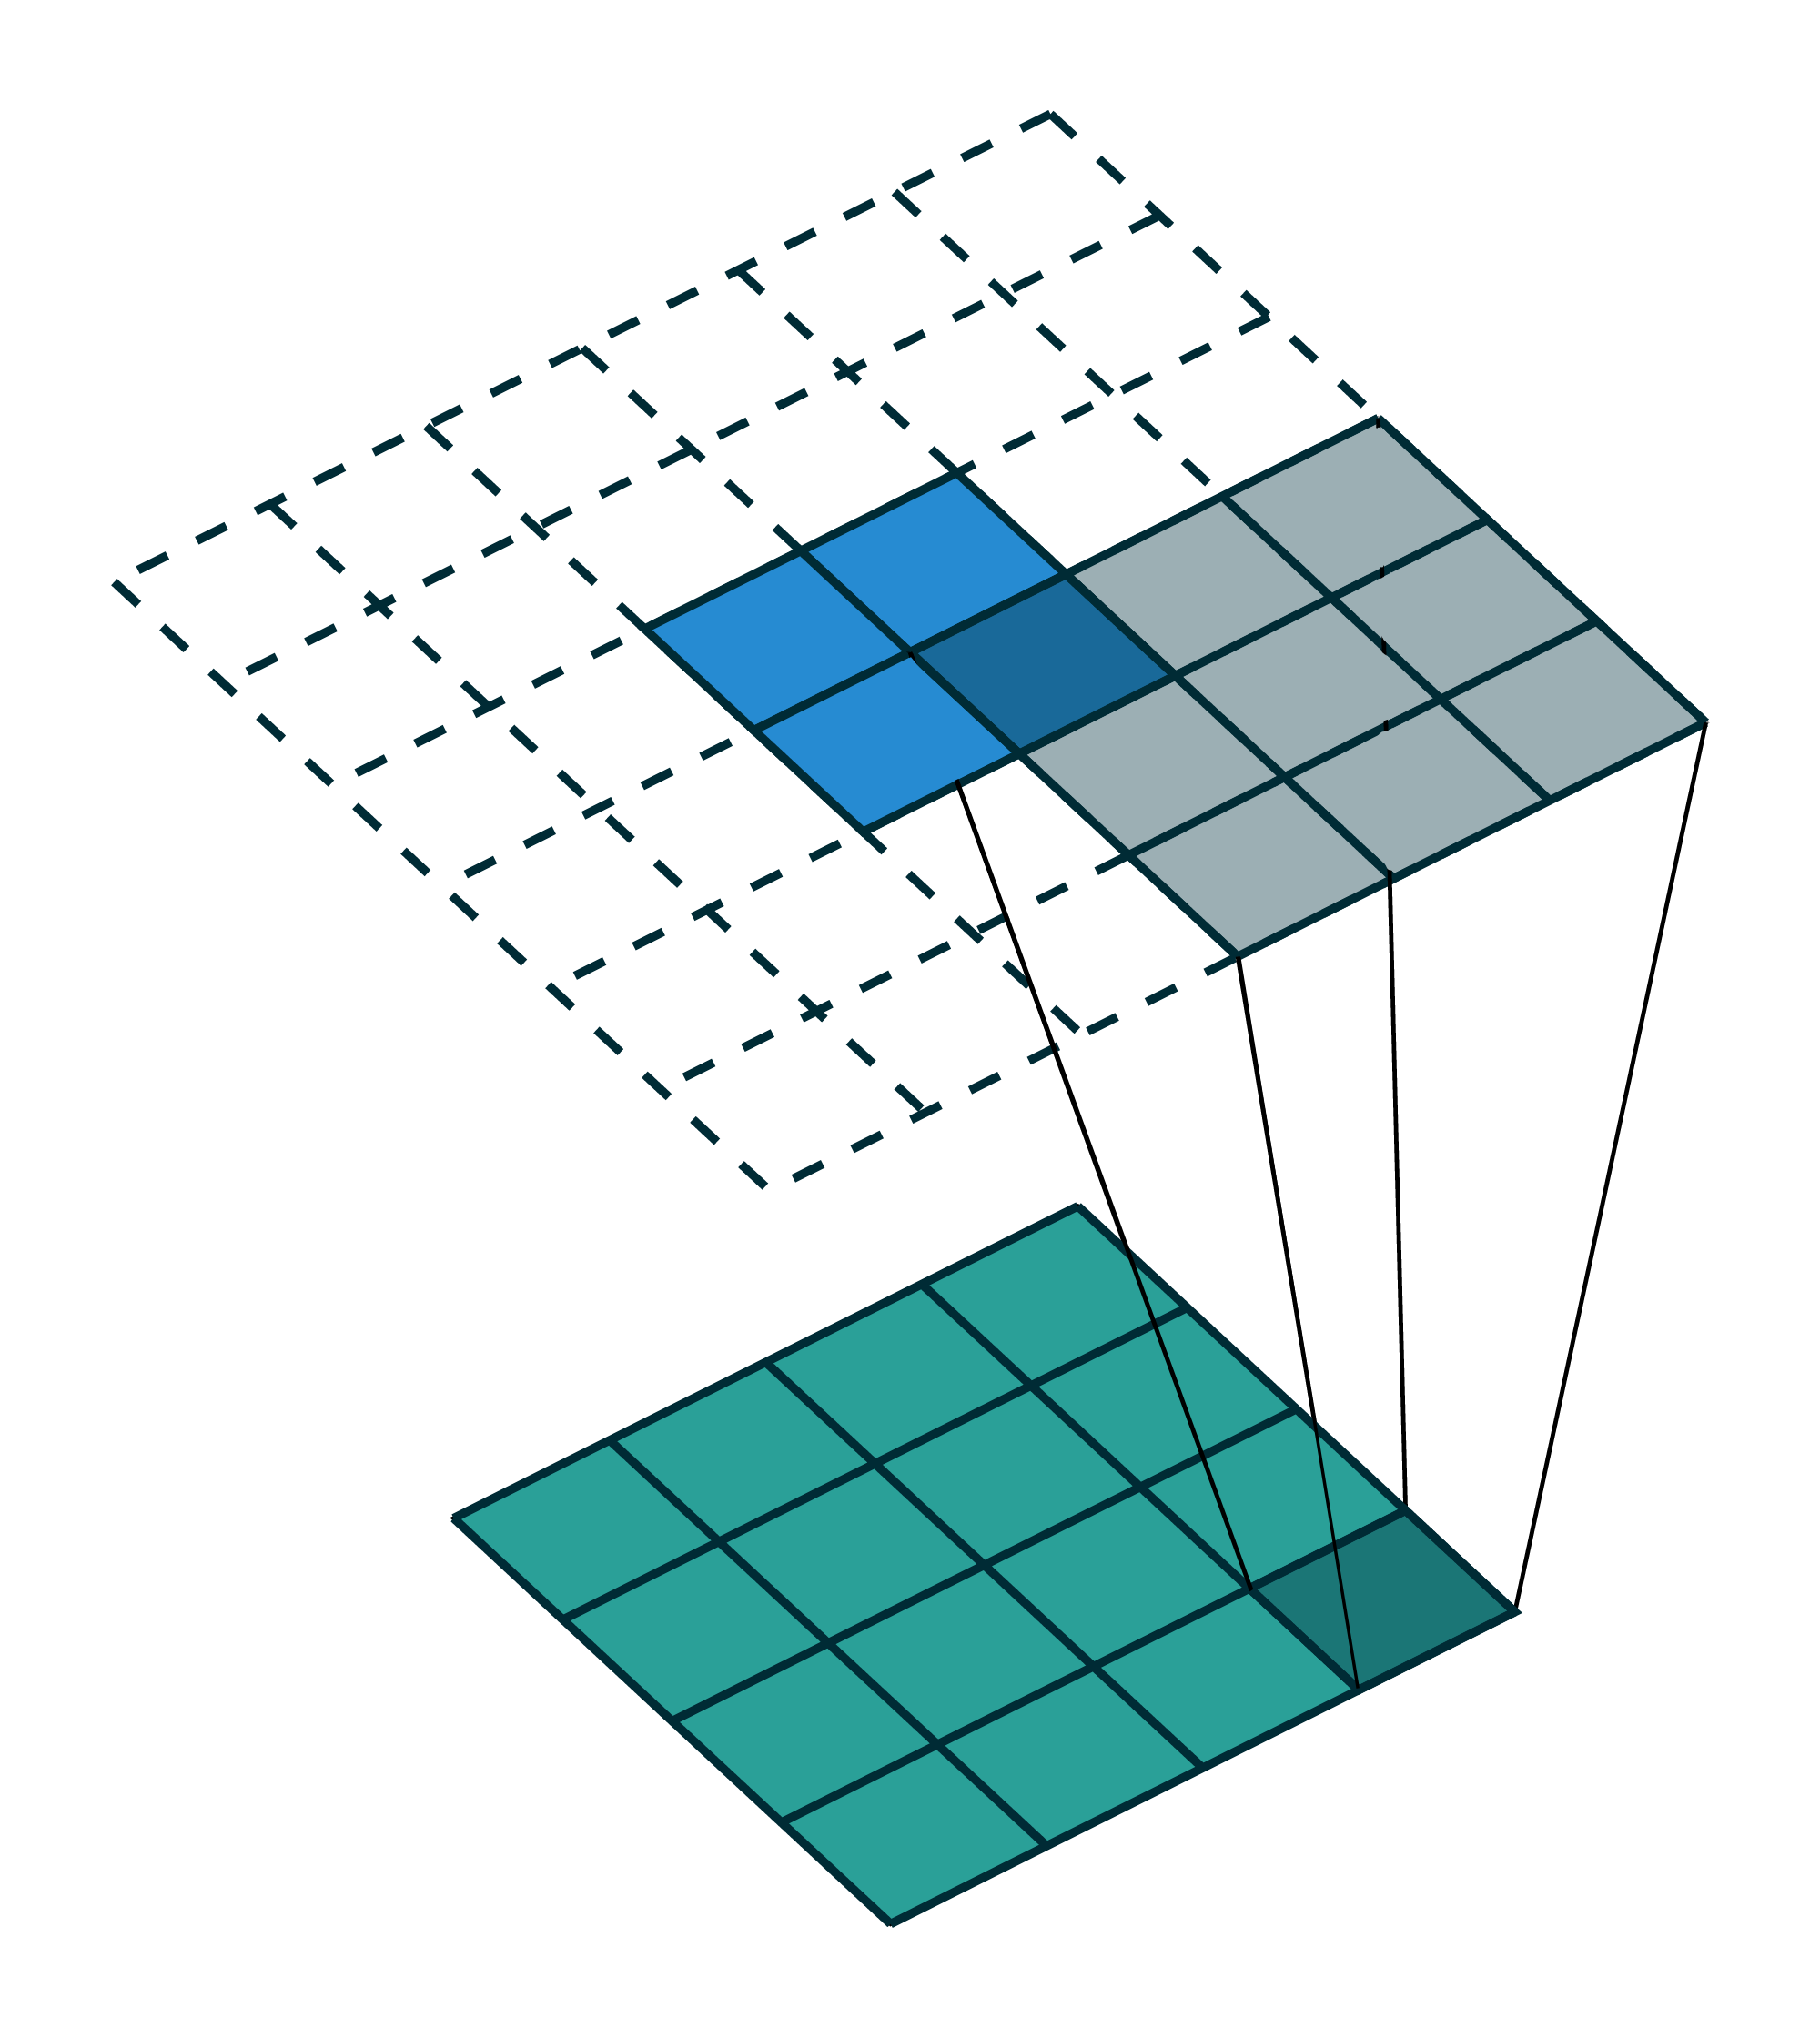
\includegraphics[width=.8\linewidth]{imgs/crbm_padding2.png}
  		\caption{The downward pass in the convolutional RBM}
  		\label{fig:convrbmsub3}
	\end{subfigure}
	\caption[A Gibbs sampling step in a convolutional RBM.]{A Gibbs sampling step in a convolutional RBM. At first the visible data is convolved with the kernel to get the hidden activations. Afterwards the kernel matrix is flipped 180\textdegree . In the downward pass the hidden activations with padding are convolved with the flipped kernel to get the new visible activations \cite{convImg}.}
	\label{fig:convrbm}
\end{figure}


Similar to a normal RBM, a convolutional RBM is trained with the objective to maximize the probability of the training data.
This can be achieved by using the CD algorithm with a few adaptations due to the tied weights (similar to backprop for CNNs in Chapter \ref{c:cnntraining}) \cite{NorouziM2009}: 
\[
\frac{\partial E}{\partial w} = \sum_{w \in W_{\text{group}}} \Delta w,
\]
where $W_{\text{group}}$ is a group of weights tied to the same value.

In contrast to CNNs, due to their local learning rule, RBMs can not be explicitly trained to perform max pooling operations.
Thus Lee et al. proposed an softmax based probabilistic max pooling to introduce local sparseness in the hidden layer activations, on top of which a pooling layer can be stacked \cite{lee2009convolutional}:
\[
P(h^k_{ij} | \textbf{v}) = \frac{\exp(I(h^k_{ij}))}{1 + \sum_{(i',j') \in B} \exp(I(h^k_{i'j'}))},
\]
where $I(h^k_{ij})$ is the activation of the hidden unit before applying the sigmoid function ( $I(h^k_{ij})=(W * \textbf{v}) + \textbf{b}_{h}$ ) and $B$ is a partition block containing the unit $h^k_{ij}$. 
Such an architecture is visualized in Fig \ref{fig:probmaxpool}.
This drives the activity in a block to be sparse and likely only one or none unit a block will be active.

\begin{figure}[h!]
	\centering
    	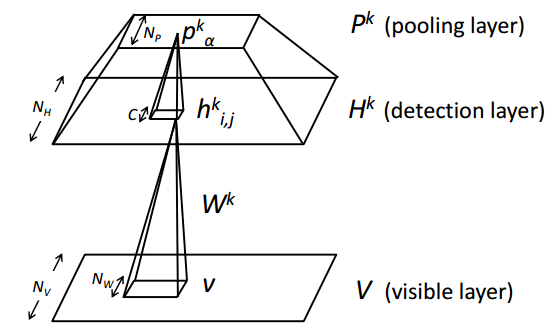
\includegraphics[width=0.4\textwidth]{imgs/prob_max_pool.png} 
    \caption{The RBM layer architecture with probabilistic max pooling \cite{lee2009convolutional}.}
	\label{fig:probmaxpool}
\end{figure}


\section{Sampling in SNNs} \label{c:snnsampling}

Indicated by stochastic neural transitions found in the brain in experimental studies, a new way of information encoding in the brain as representations of probability distributions and probabilistic interference has been suggested \cite{griffiths2008bayesian}\cite{lee2003hierarchical}\cite{yang2007probabilistic}.


A first framework, which proposed how spiking neurons can perform MCMC sampling, was introduced by Buesing \cite{Buesing2011}.
A simplification to discretize time into time slices can be introduced without interfering with the basic concept (see Buesing for the generalization to continuous time \cite{Buesing2011}).

The neuron network can be considered as a network of RVs, where the state of a neuron is defined by its firing. 
Since the probability of two neurons spiking at the same time is basically zero, after a neuron has fired it is set to the firing state for a time period $\tau$
\[
z_k(t) = 
\begin{cases}
1, &  \text{if k has fired in the time intervall } (t - \tau , t ] \\
0, &  \text{if k has not fired in the time intervall } (t - \tau , t ] 
\end{cases}
\] 
where $z_k$ is the state of neuron $k$ and set to $1$ for the "firing" state and $0$ for the "not firing" state (see Fig. \ref{fig:snnsamp1}). 
A common choice for $\tau$ is the refractory period of the neuron $\tau_{ref}$.
Consequently, one way to characterize the firing probability of a neuron is to take the ratio of the time a neuron has spent in state $z_i=1$ compared to the total timespan $T$ : $\frac{n_{\text{spikes}_i} \, \tau}{ T }$.

Thus, for a given time step $t$ the state of the network $\textbf{z}(t) = (z_1(t), ... ,z_n(t))$ is defined by the state of the individual neurons $z_i(t)$. 


\begin{figure}
	\centering
    	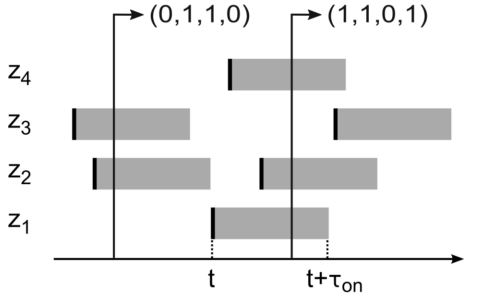
\includegraphics[width=0.4\textwidth]{imgs/snn_sample1.png} 
    \caption[A spiking neural network as probabilistic model.]{A spiking neural network as probabilistic model. The state $z_i$ of a neuron is set to $1$ for a time period $t_{on}$ after a spike. The complete state of the network $\textbf{z}$ is given by the individual state $(z_1, z_2, z_3, z_4)$  \cite{Petrovici2016}.}
	\label{fig:snnsamp1}
\end{figure}

To get a process with Markovian properties $p(z_t| (z_0, ..., z_{t-1})) = p(z_t| z_{t-1}) $, a auxiliary counter variable $\xi \in \mathbb{N}$ is introduced which discretizes the time a neuron has left to stay in the "firing" state into time slices
\[
z_k(t) = 1 \iff \xi_k(t) \ge 1
\]
Thus $\xi$ can be seen as a counter, counting down from $\tau$ to $0$ in each time step after a neuron has fired (see Fig. \ref{fig:snnsamp2} for schematic overview and a sample implementation)
\[
p(\xi_t | \xi_{t-1}) = 
\begin{cases}
	1, & \text{ for } \xi_{t-1} > 1 \text{ and } \xi_t = \xi_{t-1} -1 ,\\
	p("firing"), & \text{ for } \xi_{t-1} \le 1 \text{ and } \xi_t = \tau ,\\
	p("not firing"), & \text{ for } \xi_{t-1} \le 1 \text{ and } \xi_t = 0 ,\\
	0, & \text{otherwise}.
\end{cases}
\]

\begin{figure}
	\centering
	\begin{subfigure}[t]{.39\textwidth}
  		\centering
  		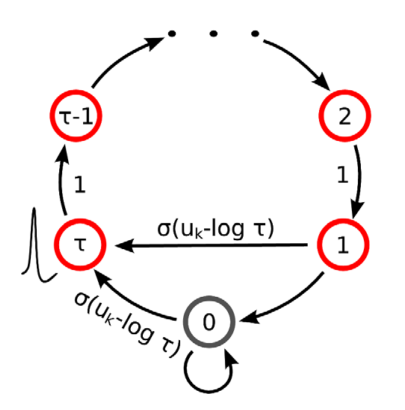
\includegraphics[width=0.9\textwidth]{imgs/snn_sample2.png}
  		\caption{}
  		\label{fig:snnsamp2sub1}
	\end{subfigure}
	\begin{subfigure}[t]{.59\textwidth}
  		\centering
  		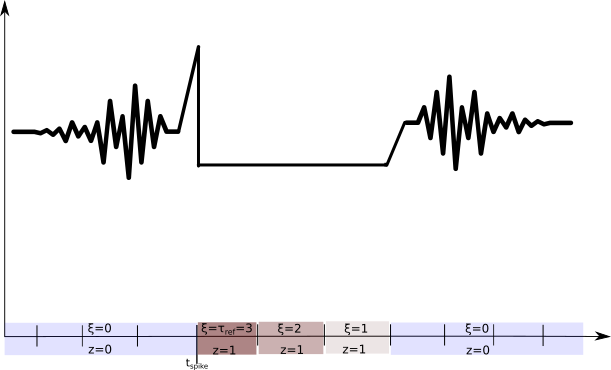
\includegraphics[width=0.9\textwidth]{imgs/sampl_bsp.png}
  		\caption{}
  		\label{fig:snnsamp2sub1}
	\end{subfigure}
    \caption[The artificial counter state of a neuron in a discrete time.]{The artificial counter state $\xi$ of a neuron in a discrete time. In (a) the red state represent an active state $z_i = 1$. After a spike $\xi$ is set to the refractory period $\tau$. In each time step the refractory period counter $\xi$ is reduced by 1 until the neuron is inactive and can spike again. In (b) a exemplary membrane potential with the corresponding states of a neuron is given \cite{Buesing2011}.}
	\label{fig:snnsamp2}
\end{figure}




Buesing proposes an abstract stochastic neuron model which activates with a probability proportional to the input
\[
P(\textit{"i fires at time t"}) \approx \sigma(\sum_j w_{ij} z_j(t) + b_i).
\]
With this model Buesing proved that spikes and the corresponding state updates in a such networks can be seen as MCMC sampling. Experiments show, as $t \rightarrow \infty$ , the network is in fact able to approximate a Boltzmann distribution.
Replacing the rectangular PSP with a more biological plausible alpha shaped PSP deteriorates the performance a little, due to overshooting at the beginning and accumulation effects, but is still reasonable well (see Fig. \ref{fig:snnsamp3}).

Petrovici improved the model by replacing the abstract stochastic neuron model by conductance bases LIF neurons, a more common and biologically inspired neuron model \cite{Petrovici2016}.
He proved under high frequency (Poisson) noise, which leads to a high conductance state of the membrane potential, the neuron shows stochastic firing, determined by the input current and the noise frequency (as described in Chapter \ref{c:hcs}).
This allows the neuron to show a firing behaviour which can be matched by a sigmoid function (see Fig. \ref{fig:snnsamp4}).  
By scaling the weights the LIF neurons can be used to perform neural sampling similar to Buesing.

\begin{figure}[h!]
	\centering
	\begin{subfigure}[t]{.50\textwidth}
  		\centering
  		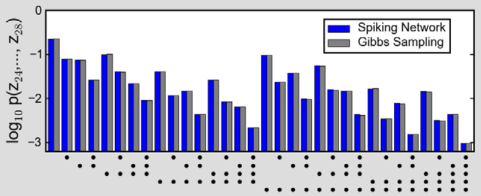
\includegraphics[width=.8\linewidth]{imgs/snn_sample3.png}
  		\caption{}
  		\label{fig:sub1}
	\end{subfigure}%
	\begin{subfigure}[t]{.50\textwidth}
  		\centering
  		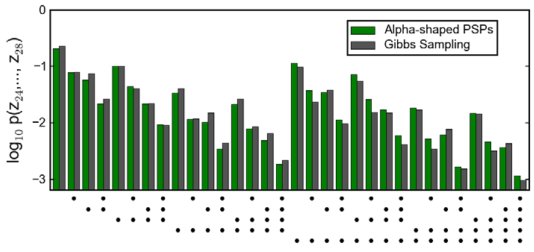
\includegraphics[width=.8\linewidth]{imgs/snn_sample4.png}
  		\caption{}
  		\label{fig:sub2}
	\end{subfigure}
	\caption[Comparison of the state probabilities of neural sampling with Gibbs sampling.]{Comparison of the state probabilities of neural sampling with Gibbs sampling in a five state Boltzmann machine. In (a) a probabilistic neuron model with a rectangular PSP is used and no discrepancies can be detected given a long enough sampling period. In (b) a more biological plausible alpha shaped kernel is used, which leads to some differences \cite{Buesing2011}.}
	\label{fig:snnsamp3}
\end{figure}


\begin{figure}
	\centering
    	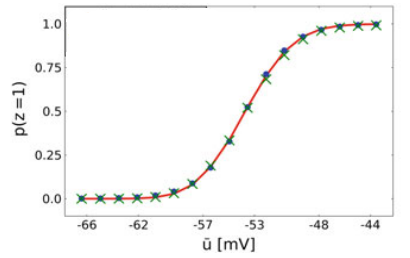
\includegraphics[width=0.4\textwidth]{imgs/snn_sample5.png} 
    \caption[Input output transfer function of a neuron in a high conductance state.]{Input output transfer function of a neuron in a high conductance state. The output rate is normalized by $\frac{1}{\tau_{ref}}$ to get a output probability. The transfer function is identical to shifted sigmoid function $\sigma$  \cite{Petrovici2016}.}
	\label{fig:snnsamp4}
\end{figure}

\section{Artificial to Spiking Neural Network Conversion} \label{c:nnconversion}

The results of Petrovici and Buesing allow a quite simple transformation of a Boltzmann machine to spiking neural networks of noisy conductance based LIF neurons with the synaptic weights scaled to match the impact on the membrane potential \cite{Petrovici2016}.
\\
\\
O'Connor uses a different approach, where instead of approximating sigmoid units by LIF neurons, he uses the Siegert neuron, a rate base approximation of LIF neurons with Poisson input, in order to implement units in the artificial RBM which activate similarly to LIF neurons \cite{OConnor2013}. 
Such a trained net can be directly transferred to an SNN.
For a neuron its firing rate can be approximated by the Siegert transformation and can be normalized by the maximal firing rate to get an activation probability, which can be adapted by the units of the RBM. 
After the RBM with the Siegert activation function is trained, the weights can be simply adapted to an SNN with LIF neurons described by the Siegert approximation.
\\
\\
There also have been several approaches to transform a CNN to an SNN.  
Cao et al. and Diehl et al. propose certain constraints on the CNN architecture to show reasonable performance in the converted SNN \cite{Cao2014}\cite{Diehl2015}:
\begin{itemize}
\item The CNN is only fed positive data since SNNs can't represent negative pre-synaptic spikes. 
\item The ReLU activation function is used in the CNN, which closely matches the input-output mapping of LIF neurons without a refractory period ( $t_{ref}=0$ ) and is always positive.
\item The bias terms are eliminated.
\item Instead of max pooling, average pooling is used, since it has a simple spiking counterpart (see \cite{Cao2014}).
\end{itemize}
After the CNN is trained with the back propagation algorithm, the weights are transferred to an SNN with an equivalent architecture using LIF neurons without a refractory period (see Fig \ref{fig:csnnconv} for an adapted CNN the equivalent SNN architecture). 
In addition, before applying the final weights, Diehl et al. use a model- and data-based weight normalization procedure to further fine-tune the synaptic weights \cite{Diehl2015}. 

\begin{figure}
	\centering
	\begin{subfigure}[t]{.80\textwidth}
  		\centering
  		\includegraphics[width=.97\linewidth]{imgs/cnn_snn_conv1.jpg}
  		\caption{A for conversion adapted CNN architecture.}
  		\label{fig:sub1}
	\end{subfigure}%
	
	\begin{subfigure}[t]{.80\textwidth}
  		\centering
  		\includegraphics[width=.97\linewidth]{imgs/cnn_snn_conv2.jpg}
  		\caption{A to an SNN converted convolutional network.}
  		\label{fig:sub2}
	\end{subfigure}
	\caption{The proposed architectures to conversion between CNNs and SNNs \cite{Cao2014}. }
	\label{fig:csnnconv}
\end{figure}

\section{Event-Driven CD} \label{c:ecd}

Different approaches to train a rate-based or spiking RBM have been proposed, of which the first was probably by Teh et al.\cite{Teh2005}.
They use multiple identical binary stochastic input units for the each element in a data sample to approximate a rate based input.

The approaches described next make use of the synaptic sampling described in the previous Chapter \ref{c:snnsampling}.

One approach is the evtCD by Neil et al., which works in continuous time with spiking networks and an STDP variant \cite{Diehl2015}.
He simulates the positive and negative phase of the CD by unrolling the RBM with shared weights (as seen in Fig. \ref{fig:evtCD} where the RBM is unrolled to simulate CD-1 updates). 
But this approach only allows a fixed number of CD steps and is, due to the weight synchronization, not very plausible.

\begin{figure}
	\centering
    	\includegraphics[width=0.4\textwidth]{imgs/evtCD.png} 
    \caption[An unrolled RBM with tied weights for CD.]{An unrolled RBM with tied weights, which can be used to simulate the positive and negative phase and learn the weighs online \cite{Neil2013}.}
	\label{fig:evtCD}
\end{figure}

A more sophisticated approach, called eCD, which also uses STDP was proposed by Neftci et al.\cite{Neftci2013}.
They use bidirectional synapses between a visible and hidden layer of LIF neurons.
They implement an adapted symmetric STDP variant, which, at a given time, only allows LTP or LDP to model the positive or negative phase of the CD algorithm respectively (see Figure \ref{fig:ecdcomp} for a comparison). 
The symmetric learning rule for two neurons, given their spike train $v_i(t)$ and $h_j(t)$, can be expressed as:
\[
\Delta w_{ij} = \mu g(t) STDP(v_i(t), h_j(t)),
\]
with the learning rule $\mu$, the global STDP status flag $g(t)$ determining the positive and negative phase of the CD algorithm and $STDP(v, h)$ parametrized to implement a symmetric weight change dependent on the neural activity:
\[
\begin{split}
STDP(v_i(t), h_j(t)) &= v_i(t) A_{h_j}(t) + h_j(t) A_{v_i}(t), \\
A_{h_j}(t) &= A \int_{- \infty}^t W(t-s) h_j(s) ds, \\ 
A_{v_i}(t) &= A \int_{- \infty}^t W(t-s) v_i(s) ds. \\ 
\end{split}
\]
In this STDP rule $A(t)$ can be seen as an activity trace indicating recent activity and $v_i(t)$ , $h_j(t)$ as a control variable enabling weight changes given a spike at time $t$.    
The kernel function $W$ should be symmetric, a common choice is $W(x) = exp(\frac{x}{\tau})$. 

\begin{figure}
	\centering
    	\includegraphics[width=0.8\textwidth]{imgs/eCD2.png} 
    \caption[Comparison between classical CD and event-based CD.]{Comparison between classical CD and event-based CD. In the classical k-CD (a) the weight update is determined by positive phase and negative phase, while in event-base CD (b) the weight update is determined by STDP and the sampling phase, determined by $g$ \cite{Neftci2013}.}
	\label{fig:ecdcomp}
\end{figure}
  
In their approach a training step can be divided into four phases (see Fig. \ref{fig:ecdph}):
\begin{enumerate}
\item The data signal is applied and the system is allowed to model the data distribution ($g(t)=0$).
\item Positive STDP is used to get $v_i h_j$-data (with LTP) and is added to the weights (postive phase $g(t)=1$).
\item The data signal is removed and the system is allowed to model the model distribution ($g(t)=0$).
\item Negative STDP is used to get $v_i h_j$-model (with LTD) and is subtracted from the synaptic weights (negative phase $g(t)=-1$).
\end{enumerate}


In similarity to RBMs, the weight change in the second phase can be summarized as $\mu \; \delta w_{pos}$, the weight change in the fourth phase as $\mu \; \delta w_{neg}$, which results in the CD update rule:
\[
w = w +  \mu \; \delta w_{pos} - \mu \; \delta w_{neg} = w +  \mu (\delta w_{pos} - \delta w_{neg}).
\]
 
 

\begin{figure}[h!]
	\centering
    	\includegraphics[width=0.3\textwidth]{imgs/eCD11.png} 
    \caption{Visualization of the phases of the event based contrastive divergence.}
	\label{fig:ecdph}
\end{figure}
\chapter{Approach} \label{c:approach}

In this section after describing the general convolutional architecture in spiking neural network in order to find the best performing spiking convolutional DBN, we discuss two different approaches to build these.

The first one is the more classical one, in which a in discrete time trained DBN is transferred to spiking neural networks.
The second approach trains the RBMs event based with STDP directly as spiking neural networks. 

In Chapter \ref{c:expres}, we will then evaluate and compare the performance of both approaches.

\section{Convolutional Architecture in Spiking Neural Networks} \label{c:spikingconvarch}

We implement a convolutional layer with receptive fields and shared weights between two neuron populations. 
Each population has a similar three dimensional topology as in artificial CNNs with the number of neurons given by $n_{ \text{neurons}} = \text{channels} \times \text{height} \times \text{width}$.

Groups of neurons in the bottom layer in close vicinity, a so-called receptive fields, are each synaptically connected to the same top layer neuron (see Fig. \ref{fig:receptfields1}).
Different receptive fields have the same shape and size $n$ and share the same synaptic weights (given the top layer neurons belong to the same feature map).
Adjacent receptive fields are overlapping by one neuron and the output neurons have the same topology as their input regions. 

A receptive field covers a partial region of the input data and the synaptic weights from the bottom layer neurons to the top layer neuron can the be seen as a convolution over the partial input data.
Since the weights of the receptive field can be shared, the neural activity in the top layer can be seen as a convolution over the input data with a filter of the size of a receptive field.
In this case the top layer activations of receptive fields with shared weights can also be called a feature map  (see Fig. \ref{fig:receptfields2}).
By using more neurons with different sets of shared weights over the same receptive fields, more feature maps can be implemented.     

\begin{figure}[h!]
	\centering
	\begin{subfigure}[t]{.4\textwidth}
  		\centering
  		\includegraphics[width=.5\linewidth]{imgs/recpt_field1.png}
  		\caption{}
  		\label{fig:receptfields1}
	\end{subfigure}%
	\begin{subfigure}[t]{.4\textwidth}
  		\centering
  		\includegraphics[width=.5\linewidth]{imgs/recpt_field2.png}
  		\caption{}
  		\label{fig:receptfields2}
	\end{subfigure}
	\caption[Receptive fields over 4 neurons.]{Receptive fields over 4 neurons. In (a) the top layer neuron (red), is only connected to a some neurons in close vicinity to each other. In (b) four receptive fields are next to each other with a stride of two and shared weights. }
	\label{fig:receptfields}
\end{figure}




\section{Conversion} \label{c:convappro}

The conversion approach can be roughly described in two steps:
\begin{enumerate}
\item Train artificial RBMs to build up an DBN.
\item Convert the DBN to a spiking neural network.
\end{enumerate}


\subsection{Convolutional DBNs} \label{c:convdbns}

To train a convolutional DBN we proceed similar to Hinton et al. and Lee et al. \cite{hinton2006fast}\cite{lee2009convolutional}.

At first the convolutional RBMs are trained greedily with CD, as described in Chapter \ref{c:convrbm}, for a certain number of iterations on data batches of batch-size $b$.
After an RBM is trained, we convert the dataset $X$ by sampling of the hidden layer of the RBM (one forward-pass step), into a new dataset $X'$:
\[
p(x') = \sigma(W * x) .
\]

On this converted dataset the next convolutional RBM is trained greedily.

Evaluating feature qualities is still an active research topic.
To get a measurement of our feature quality we use labelled data and train a classifier on top of the extracted features.
To stay in a biological plausible domain, we train a fully connected RBM on the top level features combined with the label of the data samples in order to associate the features with the correct labels.
This architecture is similar to the architecture of Hinton \cite{hinton2006fast} (see Fig. \ref{fig:dbnmnist}).

\begin{figure}
	\centering
    	\includegraphics[width=0.4\textwidth]{imgs/dbn_mnist.png} 
    \caption[A common structure of a deep belief network.]{A common structure of a deep belief network, built up of RBMs used for classification. The first layers transform the input data/ pixel image and can extract features and the top layer RBM is used for association the data with the correct label \cite{Zorzi2013Modeling}.}
	\label{fig:dbnmnist}
\end{figure}

To evaluate the final performance, we input a data sample without a label into the DBN and after a forward-pass let the top layer sample a label prediction by performing Gibbs sampling steps, which can be seen as a reconstruction of partially presented data (as mentioned in Chapter \ref{c:pgms}).


\subsection{Conversion} \label{c:conversionappr}

We present three different variations of the conversion.

\begin{figure}
	\centering
	\begin{subfigure}[t]{.5\textwidth}
  		\centering
  		\includegraphics[width=.54\linewidth]{imgs/convert_cnn.png}
  		\caption{Structure of a spiking CNN with LIF neurons.}
  		\label{fig:converted1}
	\end{subfigure}%
	\begin{subfigure}[t]{.5\textwidth}
  		\centering
  		\includegraphics[width=.8\linewidth]{imgs/convert_dbn.png}
  		\caption{Structure of a spiking DBN with LIF neurons.}
  		\label{fig:converted2}
  	\end{subfigure}
	\caption[Different converted structures of a CNN and a DBN.]{Different converted structures of a CNN and a DBN. The CNN is converted to a spiking network, by simply using simple LIF neurons (white) (a). In the DBN (b) the LIF neurons are put in a high conductance state (black), by inserting high frequency Poisson noise. The weights are scaled accordingly to fit the activations of the neurons.}
	\label{fig:converted}
\end{figure}


\paragraph{Conversion as CNN}  \label{c:convascnn}

One way to convert the DBN to the spiking domain, is by interpreting it as a pre-trained CNN with purely forward connections (we do not perform any commonly used gradient descent fine tuning to get comparable results with only CD trained models, but fine tuning could further improve the performance).
While this allows classification, it removes the generative capabilities of the network.

For the conversion, we proceed similar to Cao et al. and Diehl et al. \cite{Cao2014}\cite{Diehl2015} .
They use average pooling and ReLU functions, to get a similar architecture as SNNs.
In contrast, we don't use any pooling, since for RBM there is no simple way to integrate average pooling (used by Cao et al. and Diehl et al. in their trained CNNs), and for spiking CNNs there is no simple way to integrate probabilistic max pooling, which is to our knowledge currently the only into the training integrated pooling thought of for RBMs.
We also use the sigmoid function, since RBMs are commonly trained with sigmoid activations (but some approaches propose ReLU for RBMs as well \cite{Nair2010}).
Furthermore the input-rate output-rate transfer function of rate based LIF neurons with a refractory period matches the sigmoid function more closely.

The DBN layers are each replaced by a LIF neuron population with an identical architecture (see Fig. \ref{fig:converted1}). 
The connections are replaced by (directed) synapses and the weights of the synapses scaled with a constant factor to get similar activations.
 

\paragraph{Conversion with conductance-based LIF neurons} \label{c:convascoba}

Another way to convert the DBN to the spiking domain is by interpreting it as a directed graphical model, a sigmoid belief network, and performing ancestral sampling.
This approach is heavily based on the synaptic sampling theory, i.e. it uses spiking neurons to perform sampling.
The sampling can be either performed with current-based or conductance-base LIF neurons as described in Chapter \ref{c:snnsampling}.

For the COBA neurons, we choose a biological plausible neuron model (see parameters in Table \ref{cobalifparam}). 
The high membrane conductance, an increased Gaussian distributed mean membrane potential and thus a firing probability of $0.5$, is achieved by using high frequency Poisson generated inhibitory and excitatory spikes to get the neuron to a high conductance state (HCS) (see Fig. \ref{fig:cobahcs1}). 
This neuron model has an input-rate output-rate transfer function which approximates a sigmoid function (see Fig. \ref{fig:cobahcs2}).

The PSPs are chosen to have an alpha shape instead of a rectangular shape, which as described in Chapter \ref{c:snnsampling} may introduce some discrepancies when performing sampling compared with Gibbs sampling, but is more biologically plausible (see Fig. \ref{fig:cobahcs3}).

\begin{figure}
	\centering
	\begin{subfigure}[t]{.5\textwidth}
  		\centering
  		\includegraphics[width=.8\linewidth]{imgs/coba_lif_act.png}
  		\caption{Firing of a HCS COBA LIF neuron.}
  		\label{fig:cobahcs1}
	\end{subfigure}%
	\begin{subfigure}[t]{.5\textwidth}
  		\centering
  		\includegraphics[width=.8\linewidth]{imgs/coba_lif_sigmoid.png}
  		\caption{Input output transfer function of a HCS COBA LIF neuron.}
  		\label{fig:cobahcs2}
	\end{subfigure}
	\begin{subfigure}[t]{.5\textwidth}
  		\centering
  		\includegraphics[width=.8\linewidth]{imgs/coba_lif_bm2.png}
  		\caption{omparison between a HCS COBA LIF neuron sampling and the true distribution in a RBM.}
  		\label{fig:cobahcs3}
	\end{subfigure}
	\caption[Properties of a conductance based LIF neuron in a high conductance state.]{Properties of a conductance based LIF neuron, put into a high conductance state with high frequency input noise. The neuron fires with a probability of $0.5$ given no additional input (a). With input the input output transfer function approximates a sigmoid function (b). A network with such neurons is able to sample in a Boltzmann distribution similar to original distribution (c). }
	\label{fig:cobahcs}

\end{figure}
  
The DBN is converted by replacing each layer with a layer of conductance-based LIF neurons with Poisson noise, and the connections are transformed to synapses with the weights scaled to achieve an action function similar to the sigmoid function (see Fig. \ref{fig:converted2}).

Consequently the DBN simply performs ancestral sampling with the data sample as evidences and the label as inferred state.   


\paragraph{Conversion with current-based LIF neurons} \label{c:convascuba}

To reduce the computational expenses of the COBA models, they can be replaced by less computational complex CUBA models.
The model parameters as chose to simulate a HCS state.
Therefore the membrane time constant is reduced and the membrane conductance is increased and a static input current is inserted.  
Adding high frequency Poisson noise results in a sigmoid shaped input-rate output-rate transfer function (see Fig. \ref{fig:cubahcs}).

\begin{figure}
	\centering
	\begin{subfigure}[t]{.5\textwidth}
  		\centering
  		\includegraphics[width=.8\linewidth]{imgs/cuba_lif_act.png}
  		\caption{Firing of a HCS CUBA LIF neuron.}
  		\label{fig:sub1}
	\end{subfigure}%
	\begin{subfigure}[t]{.5\textwidth}
  		\centering
  		\includegraphics[width=.8\linewidth]{imgs/cuba_lif_sigmoid.png}
  		\caption{Input output transfer function of a HCS CUBA LIF neuron.}
  		\label{fig:sub2}
	\end{subfigure}
	\begin{subfigure}[t]{.5\textwidth}
  		\centering
  		\includegraphics[width=.8\linewidth]{imgs/cuba_lif_bm.png}
  		\caption{Comparison between a HCS CUBA LIF neuron sampling and the true distribution in a RBM.}
  		\label{fig:sub2}
	\end{subfigure}
	\caption[Properties of a current based LIF neuron in a high conductance state.]{Properties of a current based LIF neuron, put into a simulated high conductance state by high frequency input noise and a artificial high membrane conductance. The neuron also fires with a probability of $0.5$ given no additional input (a) and with input the input output transfer function approximates a sigmoid function (b). A network with such neurons can also to sample in a Boltzmann distribution similar to original distribution (c).}
	\label{fig:cubahcs}
\end{figure}
The DBN conversion is similar to the COBA case, but instead of COBA LIF neurons the adapted CUBA LIF neurons are used(see Fig. \ref{fig:converted2}).

\section{eCD} \label{c:ecdappr}

Another approach implements the training of the convolutional spiking DBN with an STDP based learning rule. 

The main idea of the learning rule is adapted from Neftcis eCD and is applied to a network of LIF neurons with symmetric bidirectional synapses \cite{Neftci2013}.
We modify the STDP learning rule described in Chapter \ref{c:ecd} by extending the model with a learning rate. 
This rule can be reformulated as an iterative rule as follows:
\begin{itemize}
\item A visible unit $v$ spikes: 
\[
\begin{split}
A_v &= A_v \exp(\frac{\Delta t}{\tau}) + a_{\delta} ,\\
A_h &= A_h \exp(\frac{\Delta t}{\tau}) ,\\
\delta w &= \mu g(t)  A_v  ,\\
\end{split}
\]
\item A hidden unit $h$ spikes: 
\[
\begin{split}
A_h &= A_h \exp(\frac{\Delta t}{\tau}) + a_{\delta} ,\\
A_v &= A_v \exp(\frac{\Delta t}{\tau}) ,\\
\delta w &= \mu  g(t) A_h  ,\\
\end{split}
\]
\end{itemize}
where $g(t)$ is the STDP status flag, $\Delta t$ is the time difference to the last previous spike, and $a_{delta}$ represents the input of the incoming spike.


The original division into four training phases poses similarities to pCD since the activity of the hidden layer of the previous step is used as starting state for the next step.
We extent the model by a 5th phase between two data samples, where the network is "flushed" thus enabling normal CD  (see Fig. \ref{fig:ecd5}):

\begin{enumerate}
\item The data signal is applied and the system is allowed to model the data distribution ($g(t)=0$).
\item Positive STDP is used to get $v_i h_j$-data and is added to the weights (postive phase $g(t)=1$).
\item The data signal is remove and the system is allowed to model the model distribution ($g(t)=0$).
\item Negative STDP is used to get $v_i h_j$-model and is subtracted from the synaptic weights (negative phase $g(t)=-1$).
\item The neural activity is "flushed" by inserting a strong negative current into the visible and hidden layer, no learning is performed ($g(t)=0$).
\end{enumerate}

\begin{figure}
	\centering
   	\includegraphics[width=0.4\textwidth]{imgs/eCD_5phases.png} 
    \caption{The five phases for a data sample in the adapted eCD algorithm. }
	\label{fig:ecd5}
\end{figure}

 
\subsection{Convolution in eCD} \label{c:ecdconv}

We implement convolutions with local receptive fields and shared weights between synapses through weight synchronization.
Since each synaptic weight has its local STDP based update rule (eCD), we have to find a way to synchronize weights between synapses of the same feature map.
To keep the shared weights the same, we perform a STDP weight synchronization step at discrete time steps, since updating all weights after a single update did not show any promising results, due to some self-reinforcement and resulting weight "explosion" (see \ref{fig:ecdnestconv} for further insight).
Thus the synchronization at a time step for weight shared weights $w_i$ , $w_j$ can be illustrated by the following rule:  
\[
\begin{split}
w_i(t) = w_{shared}(t-1) + \delta w_i, \\ 
w_j(t) = w_{shared}(t-1) + \delta w_j 
\end{split}
\]
which gives the new shared weight
\[
\begin{split}
w_{shared}(t) = \frac{1}{2} (w_i(t) + w_j(t) ) = \frac{1}{2} (w_{shared}(t-1) + \delta w_i + w_{shared}(t-1) + \delta w_j) = \\ w_{shared}(t-1) + \frac{1}{2} (\delta w_i + \delta w_j).
\end{split}
\]

This results in a update rule similar to the convolutional RBM update rule as presented in Chapter \ref{c:convrbm}.
Thus we can simply take the mean of the weight changes and apply it to all the weights, which is equivalent to just taking the average of the new individual weights. 

\paragraph{Lateral inhibition} \label{c:latinhib}
In addition we introduce fixed negative connections between neuron in the hidden layers ( which is more biologically plausible \cite{King2013}, see a simplified sample in Fig. \ref{fig:bminhib}).
This removes one advantage of RBMs since the hidden layers are no longer independent, which makes it harder to sample from the true distributions, but since the network continuously performs sampling steps, the approximation has shown to be sufficient, if the weights are not too strong and prevent changes of different modes (see Chapter \ref{c:latinhibexp} and Fig. \ref{fig:dbnmixing} ).

\begin{figure}
	\centering
    	\includegraphics[width=0.4\textwidth]{imgs/lateral_inhib.png} 
    \caption{A (restricted) Boltzmann machine with lateral inhibition in the top layer.}
	\label{fig:bminhib}
\end{figure}


Connecting neurons to neurons on a similar positions in other feature maps appears to make the features more discriminative and less correlated.
This also poses some similarities to adding a negative structured bias to the hidden units, which has shown to result in better features \cite{DBLP:journals/corr/KheradpishehGTM16}\cite{LeCun}\cite{NorouziM2009}.

An intuitive interpretation is that if one feature reacts to a certain input it will be highly active and prevent the others from being active as well and thus prevent them from learning the same features.  

\subsection{Spiking DBNs} \label{c:spikingdbn}

To build up a spiking DBN we train the convolutional BMs layer-wise and forward the input of the previous layer to the next layer.

Either replacing the symmetric bidirectional synapses with forward only synapses or keeping them bidirected, did not show any significant differences (see Fig. \ref{fig:spikingdbnarch} ). 
To be exact the spiking DBN with bidirectional synapses in the bottom RBMs is a mixture between a deep belief network and a deep Boltzmann machine, since the single Boltzmann machines are still bidirectional connected and only the hidden layer activations are forwarded in a directed manner to the next Boltzmann machines (see Fig. \ref{fig:spikedbn}).

Due to some top-down influences, when stacking a new BM  on the trained BM directly, the hidden distribution gets distorted and unfit input for the new BM to be trained on. 
To solve this in our case we use forward connections from the hidden layer of the bottom BM to the visible layer of a new two layered top BM. 
An approach to predict the influences of the top RBM in advance e.g like Salakhutdinovs DBMs by doubling the weights or joint training may sound promising and could be an area for further research \cite{salakhutdinov2009deep}.

\begin{figure}[h]
	\centering
    	\includegraphics[width=0.4\textwidth]{imgs/spike_dbm.png} 
    \caption[Structure of a deep belief network trained with eCD.]{The structure of a deep belief network trained with eCD. The spiking DBN consists of single Boltzmann machines stacked on top of each others. In contrast to artificial DBNs, the Boltzmann machines are still bidirection connected, and two Boltzmann machines are stacked up by forwarding the activations of the hidden layer in the bottom RBM to the visible layer in the top RBM.}
	\label{fig:spikedbn}
\end{figure}


\chapter{Implementation} \label{c:impl}


\section{Artifical DBNs} \label{c:dbnimpl}

The DBNs were implemented in the Theano-Framework \cite{2016arXiv160502688full}, to utilize the computational power of the GPU.
The implementation of the singe RBMs is adapted from the official Theano RBM \cite{theanoRBM}.
\\
\\
An upward pass in performed as follows:
As an input we take a 4D tensor $\textbf{V}$ of size \textit{(batch size, input channels, input rows, input columns)}, and for the upwards pass convolve it with a filters $\textbf{W}$ of the shape \textit{(number of filters, input channel, filter height, filter width)} with a stride of 1 without any padding.
This results in feature maps $\textbf{H}_{pre} = \textbf{W} * \textbf{V}$ of the shape \textit{(batch size, number of filters, input height - filter height + 1 , input width - filter width + 1)}.
A constant $c$ is added to the pre-activation feature maps as bias.
On those feature maps a sigmoid function $\sigma$ is applied and accordingly Bernoulli sampled to get the activation of the hidden units $\textbf{H}$.

\begin{algorithm}
\caption{Upward pass}
\begin{algorithmic}
\State ${H}_{pre}\gets W * V + c $  
\State ${H}_{sigmoid} \gets \sigma({H}_{pre})$
\State $H \gets {H}_{sigmoid} > Random()$
\end{algorithmic}
\end{algorithm}


The downward pass on the activation of the hidden units is performed similar:
The input is the activation of the hidden unit $\textbf{H}$ with zero padding, and convolve it with the 180 degree flipped kernel $\tilde{\textbf{W}}$, where the first and second dimensions are swapped.
Afterwards a sigmoid function $\sigma$ is applied and accordingly sampled to get the new visible layer activations $\textbf{V}'$.

\begin{algorithm}
\caption{Downward pass}
\begin{algorithmic}
\State ${V}_{pre}\gets \tilde{W} * H + c $  
\State ${V}_{sigmoid} \gets \sigma({V}_{pre})$
\State $V \gets {V}_{sigmoid} > Random()$
\end{algorithmic}
\end{algorithm}

One complete Gibbs sampling step consists of an upwards and a consecutive downward pass.

\begin{algorithm}
\caption{Gibbs step}
\begin{algorithmic}
\State $H_0 \gets upward(V_0) $  
\State $V_1 \gets downward(H_0) $  
\end{algorithmic}
\end{algorithm}

Each RBM is trained with the CD-$k$ update rule, therefore after performing one Gibbs sampling step to get a sample of the data distribution $\textbf{V}_0, \textbf{H}_0$  (positive phase), we perform $k-1$ additional Gibbs sampling steps to get a sample of an estimate of the model distribution $\textbf{V}_k, \textbf{H}_k$  (negative phase).

As error function we define the difference between the free energy of the positive phase and the negative phase.
\[
\Delta \textbf{W} = \frac{\partial F(V_k)}{\partial \textbf{W}} -  \frac{\partial F(V_0)}{\partial \textbf{W}} 
\]
We use Theanos auto-differentiation to determine the gradient and perform gradient decent with a learning rate $\mu$ and a weight decay of $\upsilon$.
\[
\textbf{W}' = \textbf{W} - \mu \Delta \textbf{W} - \upsilon \textbf{W} 
\]
A common choice for $\mu$ is $0.1$ and for $\upsilon$ is $0.003$ throughout this thesis.
We train the RBM for a given number of iterations over the dataset, with a batch size smaller than the dataset, thus performing stochastic gradient descent.

To build up the DBN each RBM is trained greedily.
After training one RBM the entire dataset is converted by doing one upwards pass in the trained RBM and using the activation of the hidden units as the new input data for the next RBM.

\begin{algorithm}
\caption{build DBN}
\begin{algorithmic}
\For{$i$  in $\#$\textit{layers}} 
\State Train $\text{RBM}_i$ on dataset $\text{ds}_i$
\State convert dataset: $\text{ds}_{i+1} = upward_i(\text{ds}_i)$ 
\EndFor
\end{algorithmic}
\end{algorithm}

Up to this time no label information is used to train any RBM, thus the learned features up to this point are trained purely unsupervised.
The last layer, the classification layer, consists of a fully connected RBM trained on the input data of the converted data set concatenated with a one-hot encoding of the label.



\section{Conversion} \label{c:conversionimpl}

To simulate the converted DBNs we use the PyNN framework with Nest as spiking network simulator \cite{10.3389/neuro.11.011.2008}\cite{Gewaltig:NEST}.
To simulate the CNN and DBN we use current and conductance based LIF neurons, respectively, see Chapter \ref{c:conversionappr} for more details.
Each unit is injected with high frequency Possion distributed excitatory and inhibitory input spikes with the frequency $\lambda_{noise}= 5000 \text{Hz}$ and synaptic weights $w_{n+}$ and $w_{n-}$ respectively.
A common choice in this thesis is $w_{n+} \approx - w_{n-} \approx 0.1$ for current-based LIF neurons and  $w_{n+} \approx - w_{n-} \approx 0.005$ for conductance-based LIF neurons.
%The parameters for the models can be seen in Table x( @TODO table).

A unit in the DBN is represented by a neuron, a layer by a neuron population.
For the connections static synapses with the scaled original weights were used. 

The input is transformed to a Poisson distributed spike trains, where the rate of the Poisson process $\lambda_{data}$ is proportional to the original data value (e.g. the image intensities). 
The input is directly fed into the bottom layer neurons with a high fixed weight $w_{in}$ to reliably generate equal spikes in the bottom layer.    

For each data sample the network is simulated for a runtime of $t$. 
To get the classification results, the spike count of all single neurons in the label layer $a_i$ is recorded and to get a label prediction the index $i$ of the most frequent spiking neuron is determined:
\[
y_{pred} = argmax_i \; a_i,
\]
with the size of the label layer being, due to the one-hot encoding of the label, equivalent to the number of different classes ($i \in \{0,..., n_{classes}\}$). 

\section{eCD} \label{c:ecdimpl}

The eCD learning was implemented in PyNN with Nest with shared synaptic weights and shared continuous STDP weight updates as well as in the Brian simulator with individual STDP weight updates and weight synchronization at discrete timesteps \cite{10.3389/neuro.11.011.2008}\cite{Gewaltig:NEST}\cite{10.3389/neuro.11.005.2008}. 
As shown in \ref{fig:ecdnestconv} due to self-facilitation leading to a weight "explosion" when using convolutional shared weight updates, we chose Brian for most of our experiments.

As neuron type LIF neurons with high frequency input noise were chosen.
Each input element $x_i \in \textbf{x}$ of a data sample $\textbf{x}$ gets transformed to Poisson distributed spikes train, with the rate $\lambda$ proportional to the input value $\lambda \propto x_i$. 

Each RBM consist of a visible and hidden layer. 
The visible layer consist of one neuron population with $n = |\textbf{x}|$ neurons representing the input, the data population. 
If needed a second neuron population representing the label input $\textbf{y}$, the label population, can be added to the visible units.
The hidden layer is an neuron population of the size  $ k = \textit{number of filters} \times (\textit{input height} - \textit{filter height} + 1) \times (\textit{input width} - \textit{filter width} + 1)$.

The data population is sparsely connected to the hidden layer with synchronized weights implementing the convolution, while the label population is fully connected to the hidden layer.
In the hidden layer we connect a neuron to other neurons in a square around same position in different feature maps with a inhibitory synapse with a fixed negative weight.

The training of the spiking RBM is performed with the adapted eCD algorithm (see \ref{c:ecdappr}).
The RBM is trained on one data sample for $t_{sample} = n \times t_{ref}$ cycles, which can, considering the different training phases, be further divided into $t_{sample} = t_{burn-in} + t_{learn} + t_{burn-in} + t_{learn} + t_{flush} = t_{pos} + t_{neg} + t_{flush}$ (with $t_{pos} = t_{neg} = t_{burn-in} + t_{learn}$ ), as visualized in Figure \ref{fig:ecd5}. 
As a result we receive the following training procedure:
\begin{itemize}

\item $t \in [0, t_{burn-in}]$ : In the first phase ("Data burn-in phase"), the visible layer is induced with a strong negative current and the data input is fed as spikes with a high synaptic weight, so that the visible layer only spikes in accordance to the input data and is unaffected from any spikes in the top layer.
The STDP learning flag is set to $g=0$, so no learning is allowed

\item $t \in (t_{burn-in} , \; t_{burn-in} + t_{learn}]$ : In the second phase ("Data distribution phase"), now the STDP learning flag is set to $g=1$ so positive learning is allowed.
This should drive the weights to represent the data distribution.

\item $t \in (t_{pos}, \;  t_{pos} + t_{burn-in}]$ : In the third phase ("Model burn-in phase"), we set the data input of the visible layer to zero and remove the induced negative current, to let it reach the model distribution.
In this phase the learning is disabled, setting the STDP learning flag to $g=0$

\item $t \in (t_{pos} + t_{burn-in}, \;  t_{pos} + t_{burn-in} + t_{learn}]$ : In the fourth phase ("Model distribution phase"), the STDP learning flag is set to $g=-1$, enabling only negative (un-)learning.
This will unlearn the model distribution.

\item $t \in (t_{pos} + t_{neg}, \;  t_{pos} + t_{neg} + t_{flush}]$ : In the optional fifth phase ("Flush phase"), we induce a strong inhibitory current to the visible and hidden layer to remove all activity and allow a fresh start in the first phase.

\end{itemize}


The weight synchronization is set at discrete time points, after $n$ training samples.
This is performed by taking the mean over all the weights, which are to be the shared.
In addition a small weight decay is introduced:
\[
W_{new} = \text{mean}(\textbf{W}_{group}) - \upsilon * \text{mean}(\textbf{W}_{group}) , 
\]
where $\upsilon$ is the weight decay rate and $\textbf{W}_{group} = (W_0 ,... W_n)$ are all the updated weights of synapses belonging to a group of synapses with the same shared weights.
\\
Each RBM is trained on $m$ data samples.
\\
After a RBM is trained, the next RBM will be trained on top of the previous RBM.
Therefore the a connection with a strong synaptic weight is established from the hidden layer of the previous RBM to the new RBM.
The original input data is still fed to the bottom RBM while the activations of hidden layer in previous RBM act as training data for the top RBM.


At test time the network is run for a fixed timespan $t_{test}$ with the test data fed to the bottom RBM.
There is no external input forwarded to the label layer while the number of spikes in the label neurons are counted.
The neuron with the most spikes represents the predicted label.  

 
\chapter{Experiments \& Results} \label{c:expres}

\section{Datasets} \label{c:datasets}
 
We evaluate our models on three different datasets.
The dataset size is primarily limited by the computational resources, such as memory and computation time. 

\subsection{Stripe Dataset} \label{c:stripes}

We generate a $10 \times 10$ pixel noisy stripe dataset with three different oriented stripes, horizontal, diagonal and vertical. 
This could represent an object similar to a pen in different orientations.
In the easiest version of this dataset the stripes always occur on the same places with some random noise (see Fig. \ref{fig:stripes1}).
A more complex version of the datasets contains the stripes randomly distributed across the whole image (see Fig. \ref{fig:stripes2}).
This dataset can be either binary or continuous (see Fig. \ref{fig:stripes3} \& \ref{fig:stripes4}).


\begin{figure}[h!]
	\centering
	\begin{subfigure}[t]{.49\textwidth}
  		\centering
  		\includegraphics[width=.85\linewidth]{imgs/stripes31.png}
  		\caption{}
  		\label{fig:stripes1}
	\end{subfigure}%
	\begin{subfigure}[t]{.49\textwidth}
  		\centering
  		\includegraphics[width=.85\linewidth]{imgs/stripes41.png}
  		\caption{}
  		\label{fig:stripes2}
	\end{subfigure}
	\begin{subfigure}[t]{.49\textwidth}
  		\centering
  		\includegraphics[width=.85\linewidth]{imgs/stripes21.png}
  		\caption{}
  		\label{fig:stripes3}
	\end{subfigure}
	\begin{subfigure}[t]{.49\textwidth}
  		\centering
  		\includegraphics[width=.85\linewidth]{imgs/stripes11.png}
  		\caption{}
  		\label{fig:stripes4}
	\end{subfigure}
	\caption[Samples from the stripe dataset.]{Samples from the $10 \times 10$ pixel stripe dataset. The stripes in (a) and (c) have the same position in the image, while the stripes in (b) and (d) can appear anywhere in the image. In (a) and (b) the images are binary , i.e a pixel value $p \in \{0,1\}$, while in (c) and (d) the values are continuous i.e $p \in \lbrack 0,1 \rbrack $.  }
	\label{fig:stripes}
\end{figure}

 
\subsection{MNIST} \label{c:mnist}

We also evaluate the models on the MNIST dataset \cite{lecun-mnisthandwrittendigit-2010}. 
The MNIST dataset consists of 60000 28x28 pixel gray images of handwritten numbers 0-9.
Samples of the dataset are given in Figure \ref{fig:mnist}.

\begin{figure}[h!]
	\centering
    	\includegraphics[width=0.50\textwidth]{imgs/mnist.png} 
    \caption[Samples from the MNIST dataset.]{Samples from the $28 \times 28$ pixel MNIST dataset \cite{lecun-mnisthandwrittendigit-2010}. The pixel values $p$ are scales to be in the interval $p \in \lbrack 0,1 \rbrack $. }
	\label{fig:mnist}
\end{figure}


\subsection{Poker-DVS} \label{c:pokerdvs}

Another dataset used in this thesis is the Poker DVS dataset \cite{serrano2013128}.
The Dataset consists of 131 poker pip symbols extracted from 3 separate DVS recordings, while quickly browsing poker cards.
From the $128 \times 128$ recorded image, a $32 \times 32$ pixel patch, containing the symbol is extracted.
As a compromise between computational and classification performance, we down sample the patches to a size of $16 \times 16$ pixels and only consider spikes in the first $8 ms$, due to the constraint learning time per sample.
The resulting dataset is visualized in Figure \ref{fig:pokerdvs} by integrating all events of a sample and then normalizing them by the maximal number of events per pixel.
 
    
\begin{figure}[h!]
	\centering
    	\includegraphics[width=0.55\textwidth]{imgs/poker_ds.png} 
    \caption[Samples from the Poker-DVS dataset.]{Visualization of samples from the Poker-DVS dataset \cite{serrano2013128}. The images are generated by integrating all events over $8$ ms. The actual training is performed on the events.}
	\label{fig:pokerdvs}
\end{figure}


\subsection{Ball-Can-Pen-DVS} \label{c:bcpdvs}

For this thesis we recorded a dataset of three different object categories with a Dynamic Vision Sensor (DVS), the Ball-Can-Pen-DVS (BCP-DVS) dataset.
Motivated by different types of grasps, balls, cans and pens were chosen.   
To generate the dataset, images of these objects were flashed for 200$ms$ at different positions on an LED-display and recorded with an DVS.
The recordings were further divided into 100$ms$ samples, which results in $90$ samples for each class. 
Similar to the Poker-DVS dataset, the $128 \times 128$ pixel samples were scaled to a size of $16 \times 16$ pixels. 

The original recorded events and the scaled events are visualized in Figure \ref{fig:bcpdvsp} by integrating all events of a sample and then normalizing them by the maximal number of events per pixel.
 
\begin{figure}[h!]
	\centering
	\includegraphics[width=0.80\textwidth]{imgs/bcp/ds1.png} 
	\caption[Pen samples from the Ball-Can-Pen-DVS dataset.]{ Recorded and down sampled samples from the Ball-Can-	Pen-DVS dataset visualized by  integrating all events of a sample and then normalizing them by the maximal number of events per pixel. Each first row shows the original sized DVS samples with the corresponding scaled samples in the second row.
	In the top rows are samples of different Balls, in the middle rows are samples of Cans and in the bottom rows are samples of Pens presented.	
	}
	\label{fig:bcpdvsp}
\end{figure} 
 
%\pagebreak 
 
%\begin{figure}[h!]
%	\centering
%	\begin{subfigure}[t]{.24\textwidth}
%  		\centering
%  		\includegraphics[width=.9\linewidth]{imgs/bcp/b1o.png}
%	\end{subfigure}%
%	\begin{subfigure}[t]{.24\textwidth}
%  		\centering
%  		\includegraphics[width=.9\linewidth]{imgs/bcp/b2o.png}
%	\end{subfigure}
%	\begin{subfigure}[t]{.24\textwidth}
%  		\centering
%  		\includegraphics[width=.9\linewidth]{imgs/bcp/b3o.png}
%	\end{subfigure}
%	\begin{subfigure}[t]{.24\textwidth}
%  		\centering
%  		\includegraphics[width=.9\linewidth]{imgs/bcp/b4o.png}
%	\end{subfigure}
%
%	\begin{subfigure}[t]{.24\textwidth}
%  		\centering
%  		\includegraphics[width=.9\linewidth]{imgs/bcp/b1.png}
%	\end{subfigure}%
%	\begin{subfigure}[t]{.24\textwidth}
%  		\centering
%  		\includegraphics[width=.9\linewidth]{imgs/bcp/b2.png}
%	\end{subfigure}
%	\begin{subfigure}[t]{.24\textwidth}
%  		\centering
%  		\includegraphics[width=.9\linewidth]{imgs/bcp/b3.png}
%	\end{subfigure}
%	\begin{subfigure}[t]{.24\textwidth}
%  		\centering
%  		\includegraphics[width=.9\linewidth]{imgs/bcp/b4.png}
%	\end{subfigure}
%		\caption[Ball samples from the Ball-Can-Pen-DVS dataset.]{ }
%	\label{fig:bcpdvsb}
%\end{figure}
%
%\begin{figure}[h!]
%	\centering
%	\begin{subfigure}[t]{.24\textwidth}
%  		\centering
%  		\includegraphics[width=.9\linewidth]{imgs/bcp/c1o.png}
%	\end{subfigure}%
%	\begin{subfigure}[t]{.24\textwidth}
%  		\centering
%  		\includegraphics[width=.9\linewidth]{imgs/bcp/c2o.png}
%	\end{subfigure}
%	\begin{subfigure}[t]{.24\textwidth}
%  		\centering
%  		\includegraphics[width=.9\linewidth]{imgs/bcp/c3o.png}
%	\end{subfigure}
%	\begin{subfigure}[t]{.24\textwidth}
%  		\centering
%  		\includegraphics[width=.9\linewidth]{imgs/bcp/c4o.png}
%	\end{subfigure}
%
%	\begin{subfigure}[t]{.24\textwidth}
%  		\centering
%  		\includegraphics[width=.9\linewidth]{imgs/bcp/c1.png}
%	\end{subfigure}%
%	\begin{subfigure}[t]{.24\textwidth}
%  		\centering
%  		\includegraphics[width=.9\linewidth]{imgs/bcp/c2.png}
%	\end{subfigure}
%	\begin{subfigure}[t]{.24\textwidth}
%  		\centering
%  		\includegraphics[width=.9\linewidth]{imgs/bcp/c3.png}
%	\end{subfigure}
%	\begin{subfigure}[t]{.24\textwidth}
%  		\centering
%  		\includegraphics[width=.9\linewidth]{imgs/bcp/c4.png}
%	\end{subfigure}
%	\caption[Can samples from the Ball-Can-Pen-DVS dataset.]{ }
%	\label{fig:bcpdvsc}
%\end{figure}
%
%\begin{figure}[h!]
%	\centering
%	\begin{subfigure}[t]{.24\textwidth}
%  		\centering
%  		\includegraphics[width=.9\linewidth]{imgs/bcp/p1o.png}
%	\end{subfigure}%
%	\begin{subfigure}[t]{.24\textwidth}
%  		\centering
%  		\includegraphics[width=.9\linewidth]{imgs/bcp/p2o.png}
%	\end{subfigure}
%	\begin{subfigure}[t]{.24\textwidth}
%  		\centering
%  		\includegraphics[width=.9\linewidth]{imgs/bcp/p3o.png}
%	\end{subfigure}
%	\begin{subfigure}[t]{.24\textwidth}
%  		\centering
%  		\includegraphics[width=.9\linewidth]{imgs/bcp/p4o.png}
%	\end{subfigure}
%
%	\begin{subfigure}[t]{.24\textwidth}
%  		\centering
%  		\includegraphics[width=.9\linewidth]{imgs/bcp/p1.png}
%	\end{subfigure}%
%	\begin{subfigure}[t]{.24\textwidth}
%  		\centering
%  		\includegraphics[width=.9\linewidth]{imgs/bcp/p2.png}
%	\end{subfigure}
%	\begin{subfigure}[t]{.24\textwidth}
%  		\centering
%  		\includegraphics[width=.9\linewidth]{imgs/bcp/p3.png}
%	\end{subfigure}
%	\begin{subfigure}[t]{.24\textwidth}
%  		\centering
%  		\includegraphics[width=.9\linewidth]{imgs/bcp/p4.png}
%	\end{subfigure}
%	\caption[Pen samples from the Ball-Can-Pen-DVS dataset.]{ Recorded and down sampled samples from the Ball-Can-Pen-DVS dataset visualized by  integrating all events of a sample and then normalizing them by the maximal number of events per pixel. In the first row shows the original sized DVS samples with the corresponding scaled samples in the second row.
%	In Figure \ref{fig:bcpdvsb} are samples of different Balls, in Figure \ref{fig:bcpdvsc} are samples of Cans and in Figure \ref{fig:bcpdvsp} are samples of Pens presented.	
%	}
%	\label{fig:bcpdvsp}
%\end{figure}



\section{Experiments} \label{c:exps}

We focus in our experiments primarily on the stripe dataset, due to time and computational constrains, which will be explained first.
Then we will look at and compare the performance of the converted models.
Afterwards, to get better insight into the eCD algorithm, we will evaluating our models on the stripe dataset and then look at the performance on other datasets for comparison and generalization.
In the end we will compare those two approaches.

\subsection{Computational Constrains} \label{c:compconstr}

Most of the experiments were executed on a quad-core processor with 3.2 GHz, 16 GB RAM and a NVidia GTX 650.

In the ANN case, CNNs can be optimized to utilize the processing units (e.g., the GPU) of most computers. 
Due to the shared weights, only one copy of each convolutional filter has to be stored. 
In addition, each feature map has to be calculated and stored as well.
Calculating a features map can be reduced to a convolution operation over the previous feature maps with a kernel, which can be implemented quite computationally efficient.
Thus the data needed for an artificial CNN is given by the size of the feature maps and the kernel matrices, the operations can be primarily reduced to convolutions.  

In contrast to CNNs, spiking networks with a convolutional structure can not utilize all of the benefits.
While the shared weights still reduce the number of learning steps needed compared to a network without shared weights, the structure is more complicated.
Due to the time dependent nature of the synapses and neurons, each single neuron and synapse has to be explicitly modelled.
While the number of neurons is equivalent to the number of elements in a feature map and thus comparable to the units in a classical CNN because all synapses have an internal state, synapses with shared weights cannot be reduced to a single synapse as in kernel matrices.
In addition to the additional computations needed for the neuron dynamics, these synapse dynamics, which do not have to be modelled in classical CNNs, can drastically increase the computational complexity.   

For example a CNN over $5 \times 5 = 25$ dimensional input data with a $4 \times 4 = 16$ kernel would result in a $2 \times 2 = 4$ feature map so the number of stored values is $45$. 
For a spiking network, in addition to modelling the $25$ dimensional input data and the $4$ feature maps as time dynamic neurons, now $(2 \times 2) \times (4 \times 4) = 64$ synapses and their dynamics have to be modelled.
This number increases quadratically as the filter size is reduced or the number of filters is increased.

Due to these constrains, the experiments primarily focus on smaller datasets and are not performed on current state-of-the-art image recognition datasets. 
Specialized neuromorphic hardware, e.g., SpiNNaker or Spikey as discussed in the "Future Work" Chapter \ref{c:neuhard}, could speed up the computations and allow the evaluation of more complex datasets.  
In addition, most spiking neural network frameworks have, in contrast to most artificial neural network frameworks, which are optimized for machine learning and speed, their main focus on biological imitation and plausibility.


\subsection{Conversion} \label{c:conversionexp}

At first we compare the three different converted DBNs as introduced in Chapter \ref{c:conversionappr}.
Therefore, an artificial DBN was trained on the MINST dataset.
The dataset was split into 50.000 training images and 10.000 images for testing.
The DBN consists of three RBMs (similar to Fig. \ref{fig:dbnmnist}), where the first RBM is convolutional with 20 filters of size $1 \times 16 \times 16$. 
The second RBM has 15 filters of size $20 \times 10 \times 10$. 
The third RBM, which can also be seen as the association layer of the DBN, is fully connected and uses the output of the second RBM as well as the labels as input data.  
Each RBM is trained for $5$ epochs with CD-$2$ over the whole dataset with a learning rate of $0.1$ and a weight decay of $0.0003$.

The resulting features of the first layer are visualized in Fig \ref{fig:rbmw}.

\begin{figure}[h!]
	\centering
    	\includegraphics[width=0.7\textwidth]{imgs/weights_rbm.png} 
    \caption{Visualized $16 \times 16$ filters of the first layer convolutional RBM of a DBN trained on the $28 \times 28$ pixel MNIST dataset.}
	\label{fig:rbmw}
\end{figure}

In the end the DBN reaches a classification performance of $82.45$ \%. 
This could be further improved by increasing the training time, fine-tuning the structure and parameters of the training algorithm of the DBN, but this was not the focus of this thesis.
An intentionally simple DBN structure was chosen due to the computational effort necessary to simulate the DBN as a spiking neural network. 


\subsubsection{Conversion comparison} \label{c:conversioncomp}

For the comparison of the conversion methods, we convert the RBM to the different spiking architectures, as described in Chapter \ref{c:conversionappr}. 
The input rate of the images are converted to Poisson spike-trains with a maximal frequency of $\lambda = 100 \text{Hz}$ .
Each input sample is simulated for $500 \text{ms}$, but we inspect how the simulated timespan affects the output later on.
Since it can take approximately one minute real time to simulation $500 \text{ms}$ of such a network, we evaluate all approaches on the same randomly drawn subset of the test set consisting of $100$ samples.

A visual inspection of the activations can be seen in Fig \ref{fig:convacts}. 
It is quite apparent that all approaches capture the basic activation characteristics. 
While the conversion as an DBN is able to simulate the activation probabilities more closely to the original DBN, the spiking CNN shows a more deterministic behaviour replicating only the essential activation structure.
To quantify those differences we calculate the Kullback-Leibler divergence between the activation, which indicates the similarity of two distributions (the lower the value, the more similar are the distributions), as seen in Table \ref{tab:kldiv}.



\begin{table}[]
\centering
\caption{Kullback-Leibler divergence between the activations in the feature maps.}
\label{tab:kldiv}
\begin{tabularx}{\textwidth}{@{}XXXX@{}}
\hline
Layer & Spiking CNN   & COBA LIF DBN & CUBA LIF DBN \\ \hline
1     & 0.014 & 0.014        & 0.014        \\
2     & 0.925 & 0.072        & 0.069        \\
3     & 0.260 & 0.170        & 0.248        \\
4     & 0.296 & 2.61         & 1.067        \\
5     & 0.624 & 1.254        & 0.445        \\ \hline
\end{tabularx}
\end{table}


\begin{table}[]
\centering
\caption{Classification performances of the converted spiking DBNs to a the artificial DBN on a subset of 100 samples.}
\label{tab:convperf}
\begin{tabularx}{\textwidth}{@{}XXXX@{}}
\hline
	 				& Classification Accuracy    & Average runtime per sample \\ \hline
DBN     			& 0.87 & 0.5 s               \\
Spiking CNN     	& 0.83 & 24.2 s                \\
COBA LIF DBN     	& 0.92 & 141.3 s                \\
CUBA LIF DBN     	& 0.93 & 30.6 s                 \\\hline
\end{tabularx}
\end{table}


%\begin{figure}
%	\centering
%	\begin{subfigure}[t]{.24\textwidth}
%  		\centering
%  		\includegraphics[width=.9\linewidth]{imgs/convert/rbm00000.png}
%  		\label{fig:sub1}
%	\end{subfigure}%
%	\begin{subfigure}[t]{.24\textwidth}
%  		\centering
%  		\includegraphics[width=.9\linewidth]{imgs/convert/cnn00000.png}
%  		\label{fig:sub2}
%	\end{subfigure}
%	\begin{subfigure}[t]{.24\textwidth}
%  		\centering
%  		\includegraphics[width=.9\linewidth]{imgs/convert/coba00000.png}
%  		\label{fig:sub2}
%	\end{subfigure}
%	\begin{subfigure}[t]{.24\textwidth}
%  		\centering
%  		\includegraphics[width=.9\linewidth]{imgs/convert/cuba00000.png}
%  		\label{fig:sub2}
%	\end{subfigure}
%	
%	\begin{subfigure}[t]{.24\textwidth}
%  		\centering
%  		\includegraphics[width=.9\linewidth]{imgs/convert/rbm00001.png}
%  		\label{fig:sub1}
%	\end{subfigure}%
%	\begin{subfigure}[t]{.24\textwidth}
%  		\centering
%  		\includegraphics[width=.9\linewidth]{imgs/convert/cnn00001.png}
%  		\label{fig:sub2}
%	\end{subfigure}
%	\begin{subfigure}[t]{.24\textwidth}
%  		\centering
%  		\includegraphics[width=.9\linewidth]{imgs/convert/coba00001.png}
%  		\label{fig:sub2}
%	\end{subfigure}
%	\begin{subfigure}[t]{.24\textwidth}
%  		\centering
%  		\includegraphics[width=.9\linewidth]{imgs/convert/cuba00001.png}
%  		\label{fig:sub2}
%	\end{subfigure}	
%
%	\begin{subfigure}[t]{.24\textwidth}
%  		\centering
%  		\includegraphics[width=.9\linewidth]{imgs/convert/rbm00002.png}
%  		\label{fig:sub1}
%	\end{subfigure}%
%	\begin{subfigure}[t]{.24\textwidth}
%  		\centering
%  		\includegraphics[width=.9\linewidth]{imgs/convert/cnn00002.png}
%  		\label{fig:sub2}
%	\end{subfigure}
%	\begin{subfigure}[t]{.24\textwidth}
%  		\centering
%  		\includegraphics[width=.9\linewidth]{imgs/convert/coba00002.png}
%  		\label{fig:sub2}
%	\end{subfigure}
%	\begin{subfigure}[t]{.24\textwidth}
%  		\centering
%  		\includegraphics[width=.9\linewidth]{imgs/convert/cuba00002.png}
%  		\label{fig:sub2}
%	\end{subfigure}	
%
%	\begin{subfigure}[t]{.24\textwidth}
%  		\centering
%  		\includegraphics[width=.9\linewidth]{imgs/convert/rbm00003.png}
%  		\label{fig:sub1}
%	\end{subfigure}%
%	\begin{subfigure}[t]{.24\textwidth}
%  		\centering
%  		\includegraphics[width=.9\linewidth]{imgs/convert/cnn00003.png}
%  		\label{fig:sub2}
%	\end{subfigure}
%	\begin{subfigure}[t]{.24\textwidth}
%  		\centering
%  		\includegraphics[width=.9\linewidth]{imgs/convert/coba00003.png}
%  		\label{fig:sub2}
%	\end{subfigure}
%	\begin{subfigure}[t]{.24\textwidth}
%  		\centering
%  		\includegraphics[width=.9\linewidth]{imgs/convert/cuba00003.png}
%  		\label{fig:sub2}
%	\end{subfigure}	
%
%	\begin{subfigure}[t]{.24\textwidth}
%  		\centering
%  		\includegraphics[width=.9\linewidth]{imgs/convert/rbm00004.png}
%  		\caption{artificial DBN.}
%  		\label{fig:sub1}
%	\end{subfigure}%
%	\begin{subfigure}[t]{.24\textwidth}
%  		\centering
%  		\includegraphics[width=.9\linewidth]{imgs/convert/cnn00004.png}
%  		\caption{spiking CNN.}
%  		\label{fig:sub2}
%	\end{subfigure}
%	\begin{subfigure}[t]{.24\textwidth}
%  		\centering
%  		\includegraphics[width=.9\linewidth]{imgs/convert/coba00004.png}
%  		\caption{COBA LIF DBN.}
%  		\label{fig:sub2}
%	\end{subfigure}
%	\begin{subfigure}[t]{.24\textwidth}
%  		\centering
%  		\includegraphics[width=.9\linewidth]{imgs/convert/cuba00004.png}
%  		\caption{CUBA LIF DBN.}
%  		\label{fig:sub2}
%	\end{subfigure}	
%	\caption{Activations in the features maps in a artificial convolutional DBN and the converted spiking network architectures. }
%	\label{fig:convacts}
%\end{figure}


\begin{figure}[h!]
	\centering
	\includegraphics[width=\textwidth]{imgs/convert/compl4.png}
	\caption{Activations in the features maps in a artificial convolutional DBN and the converted spiking network architectures. }
	\label{fig:convacts}
\end{figure}

\begin{figure}[h!]
	\centering
	\begin{subfigure}{.24\textwidth}
  		\centering
  		\includegraphics[width=0.6\linewidth]{imgs/convert/err/err1.png}
  		\label{fig:sub1}
	\end{subfigure}%
	\begin{subfigure}{.24\textwidth}
  		\centering
  		\includegraphics[width=0.6\linewidth]{imgs/convert/err/err2.png}
  		\label{fig:sub1}
	\end{subfigure}%
	\begin{subfigure}{.24\textwidth}
  		\centering
  		\includegraphics[width=0.6\linewidth]{imgs/convert/err/err4.png}
  		\label{fig:sub1}
	\end{subfigure}%
	\begin{subfigure}{.24\textwidth}
  		\centering
  		\includegraphics[width=0.6\linewidth]{imgs/convert/err/err3.png}
  		\label{fig:sub1}
	\end{subfigure}%
	
	
	\caption[Misclassifications of the converted spiking DBNs on MNIST.]{Misclassifications of the converted spiking DBNs on MNIST. Often $9$ and $4$ are mixed up. The first three are classified as a $9$, the fourth one is classified as a $4$. The images all share a lot of features with the suggested class and the correct class was always the second most probable.}
	\label{fig:mismnisthum}
\end{figure}


%
%\begin{figure}
%	\centering
%	\begin{subfigure}[t]{.32\textwidth}
%  		\centering
%  		\includegraphics[width=.9\linewidth]{imgs/convert/rbm00000.png}
%  		\caption{Input data.}
%  		\label{fig:sub1}
%	\end{subfigure}%
%	\begin{subfigure}[t]{.32\textwidth}
%  		\centering
%  		\includegraphics[width=.9\linewidth]{imgs/convert/rbm00001.png}
%  		\caption{Activations in the features maps of the first RBM layer.}
%  		\label{fig:sub2}
%	\end{subfigure}
%	\begin{subfigure}[t]{.32\textwidth}
%  		\centering
%  		\includegraphics[width=.9\linewidth]{imgs/convert/rbm00002.png}
%  		\caption{Activations in the features maps of the second RBM layer.}
%  		\label{fig:sub2}
%	\end{subfigure}
%	\begin{subfigure}[t]{.32\textwidth}
%  		\centering
%  		\includegraphics[width=.9\linewidth]{imgs/convert/rbm00003.png}
%  		\caption{Activations in the features maps of the third RBM layer.}
%  		\label{fig:sub2}
%	\end{subfigure}	
%	\begin{subfigure}[t]{.32\textwidth}
%  		\centering
%  		\includegraphics[width=.9\linewidth]{imgs/convert/rbm00004.png}
%  		\caption{Activations in the features maps of the fourth/label layer.}
%  		\label{fig:sub2}
%	\end{subfigure}
%	\caption{Activations in the features maps in a classical convolutional RBM. }
%	\label{fig:stripes}
%\end{figure}
%
%\begin{figure}
%	\centering
%	\begin{subfigure}[t]{.32\textwidth}
%  		\centering
%  		\includegraphics[width=.9\linewidth]{imgs/convert/cnn00000.png}
%  		\caption{Input data.}
%  		\label{fig:sub1}
%	\end{subfigure}%
%	\begin{subfigure}[t]{.32\textwidth}
%  		\centering
%  		\includegraphics[width=.9\linewidth]{imgs/convert/cnn00001.png}
%  		\caption{Activations in the features maps of the first RBM layer.}
%  		\label{fig:sub2}
%	\end{subfigure}
%	\begin{subfigure}[t]{.32\textwidth}
%  		\centering
%  		\includegraphics[width=.9\linewidth]{imgs/convert/cnn00002.png}
%  		\caption{Activations in the features maps of the second RBM layer.}
%  		\label{fig:sub2}
%	\end{subfigure}
%	\begin{subfigure}[t]{.32\textwidth}
%  		\centering
%  		\includegraphics[width=.9\linewidth]{imgs/convert/cnn00003.png}
%  		\caption{Activations in the features maps of the third RBM layer.}
%  		\label{fig:sub2}
%	\end{subfigure}	
%	\begin{subfigure}[t]{.32\textwidth}
%  		\centering
%  		\includegraphics[width=.9\linewidth]{imgs/convert/cnn00004.png}
%  		\caption{Activations in the features maps of the fourth/label layer.}
%  		\label{fig:sub2}
%	\end{subfigure}
%	\caption{Activations in the features maps in the as CNN converted RBM. }
%	\label{fig:stripes}
%\end{figure}
%
%\begin{figure}
%	\centering
%	\begin{subfigure}[t]{.32\textwidth}
%  		\centering
%  		\includegraphics[width=.9\linewidth]{imgs/convert/coba00000.png}
%  		\caption{Input data.}
%  		\label{fig:sub1}
%	\end{subfigure}%
%	\begin{subfigure}[t]{.32\textwidth}
%  		\centering
%  		\includegraphics[width=.9\linewidth]{imgs/convert/coba00001.png}
%  		\caption{Activations in the features maps of the first RBM layer.}
%  		\label{fig:sub2}
%	\end{subfigure}
%	\begin{subfigure}[t]{.32\textwidth}
%  		\centering
%  		\includegraphics[width=.9\linewidth]{imgs/convert/coba00002.png}
%  		\caption{Activations in the features maps of the second RBM layer.}
%  		\label{fig:sub2}
%	\end{subfigure}
%	\begin{subfigure}[t]{.32\textwidth}
%  		\centering
%  		\includegraphics[width=.9\linewidth]{imgs/convert/coba00003.png}
%  		\caption{Activations in the features maps of the third RBM layer.}
%  		\label{fig:sub2}
%	\end{subfigure}	
%	\begin{subfigure}[t]{.32\textwidth}
%  		\centering
%  		\includegraphics[width=.9\linewidth]{imgs/convert/coba00004.png}
%  		\caption{Activations in the features maps of the fourth/label layer.}
%  		\label{fig:sub2}
%	\end{subfigure}
%	\caption{Activations in the features maps in a as DBN converted RBM with conductance based LIF neurons. }
%	\label{fig:stripes}
%\end{figure}
%
%\begin{figure}
%	\centering
%	\begin{subfigure}[t]{.32\textwidth}
%  		\centering
%  		\includegraphics[width=.9\linewidth]{imgs/convert/cuba00000.png}
%  		\caption{Input data.}
%  		\label{fig:sub1}
%	\end{subfigure}%
%	\begin{subfigure}[t]{.32\textwidth}
%  		\centering
%  		\includegraphics[width=.9\linewidth]{imgs/convert/cuba00001.png}
%  		\caption{Activations in the features maps of the first RBM layer.}
%  		\label{fig:sub2}
%	\end{subfigure}
%	\begin{subfigure}[t]{.32\textwidth}
%  		\centering
%  		\includegraphics[width=.9\linewidth]{imgs/convert/cuba00002.png}
%  		\caption{Activations in the features maps of the second RBM layer.}
%  		\label{fig:sub2}
%	\end{subfigure}
%	\begin{subfigure}[t]{.32\textwidth}
%  		\centering
%  		\includegraphics[width=.9\linewidth]{imgs/convert/cuba00003.png}
%  		\caption{Activations in the features maps of the third RBM layer.}
%  		\label{fig:sub2}
%	\end{subfigure}	
%	\begin{subfigure}[t]{.32\textwidth}
%  		\centering
%  		\includegraphics[width=.9\linewidth]{imgs/convert/cuba00004.png}
%  		\caption{Activations in the features maps of the fourth/label layer.}
%  		\label{fig:sub2}
%	\end{subfigure}
%	\caption{Activations in the features maps in a as DBN converted RBM with current based LIF neurons. }
%	\label{fig:stripes}
%\end{figure}

The performance on the partial dataset can be seen in Table \ref{tab:convperf}.
It is apparent that all approaches show a similar performance. Interestingly the spiking DBN sometimes shows better performance than the RBM.
Most misclassifications can from a human perspective be categorized as "reasonable" mistakes (as seen in Fig. \ref{fig:mismnisthum}) and hint, that further fine-tuning of the DBN could resolve some misclassifications.

Another factor is the simulated runtime for each sample. 
It is quite apparent from Table \ref{tab:pervovert} that a longer classification time benefits the performance.


\begin{table}[]
\centering
\caption{Classification performances of the converted spiking DBNs with different simulated runtimes.}
\label{tab:pervovert}
\begin{tabularx}{\textwidth}{l|ll|ll}
\hline
	 				& \multicolumn{2}{l}{Spiking CNN}   & \multicolumn{2}{|l}{CUBA LIF DBN} \\ \hline
Simulated time		 				& Classification Accuracy    & Runtime & Classification Accuracy    & Runtime \\ \hline
50 ms    	& 0.69 & 7.8 s 		& 0.81 & 8.1 s               \\
100 ms     	& 0.77 & 9.2 s  	& 0.89 & 10.5 s              \\
200 ms    	& 0.76 & 13.1 s   & 0.89 & 14.6 s             \\
300 ms    	& 0.75 & 15.1 s   & 0.91 & 18.5 s             \\
500 ms     	& 0.83 & 24.2 s    & 0.93 & 30.6 s             \\\hline
\end{tabularx}
\end{table}

In contrast to this approach in which the network is trained in discrete timesteps, next we look at the performance on networks trained in continuous time.  

\subsection{eCD} \label{c:ecdexp}

To get an intuitive insight into the eCD algorithm, we visualize the positive and negative phase for the stripe dataset.
It is apparent that in the positive phase a sample from the data distribution is learned and in the negative phase the model distribution is unlearned (see Fig. \ref{fig:ecdstrlearn}).
As the training progresses and the model distribution approximates the data distribution more closely the weight updates become smaller (see Fig. \ref{fig:ecdwdiff}). 
The eCD-parameters chosen for most of our experiments are given in Table \ref{tab:ecdrunparam}.

This indicates some learning and we further inspect the capability of this algorithm to learn the data distribution.

\begin{table}[]
\caption{eCD-parameters for most experiments.}
\centering
\label{tab:ecdrunparam}
\begin{tabular}{|ll|}
\hline
$t_{burn-in}$    	& 14 ms 		    \\
$t_{learn}$    		& 56 ms 		     \\
$t_{flush}$    		& 28 ms		             \\
Learn-rate     		& 1.0 		                 \\
Weight-decay    	& 0.001		              \\
Weight synchronization after $n$ samples     	& 1		              \\\hline
\end{tabular}
\end{table}


\begin{figure}[h!]
	\centering
%	\begin{subfigure}[t]{.19\textwidth}
%  		\centering
%  		\includegraphics[width=\linewidth]{imgs/inspect/00010.png}
%  		\label{fig:sub1}
%	\end{subfigure}%
%	\begin{subfigure}[t]{.19\textwidth}
% 		\centering
%  		\includegraphics[width=\linewidth]{imgs/inspect/00011.png}
%  		\label{fig:sub1}
%	\end{subfigure}%
%	\begin{subfigure}[t]{.19\textwidth}
%  		\centering
%  		\includegraphics[width=\linewidth]{imgs/inspect/00012.png}
%  		\label{fig:sub1}
%	\end{subfigure}%
%	\begin{subfigure}[t]{.19\textwidth}
%  		\centering
%  		\includegraphics[width=\linewidth]{imgs/inspect/00013.png}
%  		\label{fig:sub1}
%	\end{subfigure}%
%	
%	\begin{subfigure}[t]{.19\textwidth}
%  		\centering
%  		\includegraphics[width=\linewidth]{imgs/inspect/00014.png}
%  		\label{fig:sub1}
%	\end{subfigure}%
%	
%	\begin{subfigure}[t]{.19\textwidth}
%  		\centering
%  		\includegraphics[width=\linewidth]{imgs/inspect/00015.png}
%  		\label{fig:sub1}
%	\end{subfigure}%
%	\begin{subfigure}[t]{.19\textwidth}
%  		\centering
%  		\includegraphics[width=\linewidth]{imgs/inspect/00016.png}
%  		\label{fig:sub1}
%	\end{subfigure}%
%	\begin{subfigure}[t]{.19\textwidth}
%  		\centering
%  		\includegraphics[width=\linewidth]{imgs/inspect/00017.png}
%  		\label{fig:sub1}
%	\end{subfigure}%
%	\begin{subfigure}[t]{.19\textwidth}
%  		\centering
%  		\includegraphics[width=\linewidth]{imgs/inspect/00018.png}
%  		\label{fig:sub1}
%	\end{subfigure}%
	\includegraphics[width=.9\linewidth]{imgs/inspect/compl.png}
	\caption[Positive phase and negative phase of a diagonal stripe with 4 filters.]{Positive phase and negative phase of a diagonal stripe with 4 filters. In the first 4 images sets a stripe is learned, while during the last 4 images the model distribution is unlearned.}
	\label{fig:ecdstrlearn}
\end{figure}

\begin{figure}[h!]
	\centering
    	\includegraphics[width=0.5\textwidth]{imgs/inspect/wdiff.png} 
    \caption[Weight change during training.]{Accumulated weight change for each training sample. As more samples are presented and the weights specialize, the total weight updates decrease.}
	\label{fig:ecdwdiff}
\end{figure}



\subsubsection{Learning the data distribution} \label{c:datadistexp}

To evaluate how good the model distribution matches the data distribution, we compare the input sample to the reconstruction obtained after the removing the input and letting the system settle towards it's model distribution.
This is visualized in Figure \ref{fig:posnegstrec} and \ref{fig:actdevstr}.
In the beginning of the training the model distribution and thus the reconstruction is approximately random.
As the training progresses, the reconstruction matches the original input image more closely and thus the model distribution shifts towards the data distribution.

\begin{figure}[h!]
	\centering
	\begin{subfigure}{.25\textwidth}
  		\centering
  		\includegraphics[width=0.8\linewidth]{imgs/reconst/00001.png}
  		\label{fig:sub1}
	\end{subfigure}%
	\begin{subfigure}{.25\textwidth}
  		\centering
  		\includegraphics[width=0.8\linewidth]{imgs/reconst/00003.png}
  		\label{fig:sub1}
	\end{subfigure}%
	\begin{subfigure}{.25\textwidth}
  		\centering
  		\includegraphics[width=0.8\linewidth]{imgs/reconst/00005.png}
  		\label{fig:sub1}
	\end{subfigure}%
	\begin{subfigure}{.25\textwidth}
  		\centering
  		\includegraphics[width=0.8\linewidth]{imgs/reconst/00007.png}
  		\label{fig:sub1}
	\end{subfigure}%
	
	
	\begin{subfigure}{.25\textwidth}
  		\centering
  		\includegraphics[width=0.8\linewidth]{imgs/reconst/00002.png}
  		\label{fig:sub1}
	\end{subfigure}%
	\begin{subfigure}{.25\textwidth}
  		\centering
  		\includegraphics[width=0.8\linewidth]{imgs/reconst/00004.png}
  		\label{fig:sub1}
	\end{subfigure}%
	\begin{subfigure}{.25\textwidth}
  		\centering
  		\includegraphics[width=0.8\linewidth]{imgs/reconst/00006.png}
  		\label{fig:sub1}
	\end{subfigure}%
	\begin{subfigure}{.25\textwidth}
  		\centering
  		\includegraphics[width=0.8\linewidth]{imgs/reconst/00008.png}
  		\label{fig:sub1}
	\end{subfigure}%
	\caption[Visualization of the spikes in the visible layer during the positive phase and negative phase of a diagonal stripe.]{Visualization of the spikes in the visible layer during the positive phase and negative phase of a diagonal stripe. In the first column, at the beginning of the training, in the negative phase the network is not able to reconstruct the data distribution. As the training progresses (in the second and third column), the reconstruction approximates the original data sample more closely and is in the last column nearly perfect.}
	\label{fig:posnegstrec}
\end{figure}

In addition, the filters become more specialized, thus resulting in a sparse activation of the hidden layer as shown in Figure \ref{fig:actdevstr}.  

\begin{figure}[h!]
	\centering
	\begin{subfigure}[t]{.32\textwidth}
  		\centering
  		\includegraphics[width=.9\linewidth]{imgs/reconst/00030_h.png}
  		\caption{Spikes at the beginning.}
  		\label{fig:sub1}
	\end{subfigure}%
	\begin{subfigure}[t]{.32\textwidth}
  		\centering
  		\includegraphics[width=.9\linewidth]{imgs/reconst/00975_h.png}
  		\caption{Spikes after some training.}
  		\label{fig:sub2}
	\end{subfigure}
	\begin{subfigure}[t]{.32\textwidth}
  		\centering
  		\includegraphics[width=.9\linewidth]{imgs/reconst/hact.png}
  		\caption{Total number of spikes per sample over time.}
  		\label{fig:sub2}
	\end{subfigure}
	\caption[Spikes in the hidden layer of a spiking convolutional RBM.]{Spikes in the hidden layer of a spiking convolutional RBM. At the start of the training (a) is appears mostly random, while after training the activations become more sparse ((b) and (c))  and certain neurons become specialized on certain input patterns (b).}
	\label{fig:actdevstr}
\end{figure}

As it turns out, to approximate the data distribution and to learn discriminative features, especially in the convolutional case, lateral connections can be used.

\subsubsection{Lateral connections} \label{c:latinhibexp}

An important addition to the convolution spiking RBM are the lateral inhibitory connections in the hidden layer. 
Each neuron in the hidden layer at position $i,j$ in feature map $k$ is connected to other neurons in all other feature maps $K \setminus k$ at the approximately same position $i', j'$ with $ |i'-i| \le 2 , |j' - j| \le 2 $.   
This results in faster training and more discriminative features and better results (see Fig. \ref{fig:latconstr} for the learned weights of both approaches).

\begin{figure}[h!]
	\centering
	\begin{subfigure}[t]{.45\textwidth}
  		\centering
  		\includegraphics[width=.9\linewidth]{imgs/inhib/02129.png}
  		\caption{}
  		\label{fig:sub1}
	\end{subfigure}%
	\begin{subfigure}[t]{.45\textwidth}
  		\centering
  		\includegraphics[width=.9\linewidth]{imgs/inhib/03023.png}
  		\caption{}
  		\label{fig:sub2}
	\end{subfigure}
	\caption[$5 \times 5$ convolution filter matrices with and without lateral inhibitory connections in the top RBM layer on the stripe dataset.]{$5 \times 5$ convolution filter matrices with and without lateral inhibitory connections in the top RBM layer on the stripe dataset. In (a) the weight are trained without lateral inhibitory connections and in (b) they are trained with lateral inhibitory connections. Whereas the filters without lateral connections (a) look more similar the filters with lateral connections (b) are more different and discriminative. }
	\label{fig:latconstr}
\end{figure}

By using the lateral connection we can get some insight into the benefits of a convolutional architecture.

\subsubsection{Convolution vs. no Convolution} \label{c:convvsnoconvexp}

To demonstrate the benefits of convolution even on a small dataset, we train two DBNs with the same number of free parameters, one convolutional, one without any convolution.
The parameters for the first layer are chosen to be $20$ and for the second "association" layer $250$.

For the convolution DBN this results in a structure of $3$ $7x7$ convolutional filters in the first layer and a fully connected RBM with $5$ hidden units in the second layer.
For the DBN without convolution, this results in two fully connected RBMs, where the first RBM has $2$ hidden units and the second RBM has $120$ hidden units.

Both DBNs are trained with 100 samples for the first layer and 500 samples with labels for the second layer, since it has more free parameters.
The resulting weights are visualized in Fig. \ref{fig:wwoconwconv}.

\begin{figure}[h!]
	\centering
	\begin{subfigure}[t]{.45\textwidth}
  		\centering
  		\includegraphics[width=.9\linewidth]{imgs/cvsnc/wc.png}
  		\caption{Weights of the DBN with convolutions.}
  		\label{fig:sub1}
	\end{subfigure}%
	\begin{subfigure}[t]{.45\textwidth}
  		\centering
  		\includegraphics[width=.9\linewidth]{imgs/cvsnc/wnc.png}
  		\caption{Weights of the DBN without convolutions.}
  		\label{fig:sub2}
	\end{subfigure}
	\caption[Weights of the first layers of the DBNs with and without convolutions with the same number of free parameters.]{Weights of the first layers of the DBNs with and without convolutions with the same number of free parameters. In (a) are weights of the DBN with convolutions visualized and in (b) the weights of the DBN without convolutions.}
	\label{fig:wwoconwconv}
\end{figure}


This suggests that the DBN with convolution is able to capture the structure of the data better with the same number of free parameters. 
This is also apparent in the final classification results.
While the DBN without convolutions reaches its top performance of $60 \%$ after 500 samples, the convolutional DBN reaches its top performance of $100 \%$ already after being presented with 300 samples.
One disadvantage of convolutions is the increased runtime, which we inspect in the next section.

\subsubsection{Simulation time} \label{c:simtimeexp}

We also evaluate how the simulation time for one time step changes as the network complexity increases.
A network on the $10 \times 10$ pixel stripe dataset is run for 1 learning step, which simulates a time of $168$ms, and the runtime is measured.
As we increase the number of hidden units, the runtime increases more or less linearly (see Fig \ref{fig:simtime}).

\begin{figure}[h!]
	\centering
    	\includegraphics[width=0.65\textwidth]{imgs/runtime-1.png} 
    \caption[The runtime of a learning step in dependence on the network size.]{The runtime of a learning step in dependence on the network size. While the simulated time of $168$ms stays constant, the runtime increases linearly with the number of hidden units. If the blue line matched the red line, the simulation could be performed in realtime.}
	\label{fig:simtime}
\end{figure}

After inspecting some mechanisms and properties of the eCD algorithm, we next look at the performance of more complex DBNs trained with eCD on different datasets.

\subsubsection{Performance on the stripe dataset} \label{c:stripeexp}

The DBN consists of two layers with the first layer consisting of a convolutional RBM with $20$ filters of size $7 \times 7$ and the second layer being fully connected with $20$ hidden units (see Fig \ref{fig:dbnstrarch} for the abstract architecture).
The first layer is trained with $1000$ samples without labels.
The weights of the first layer are then keep fixed and the second layer is trained over $500$ samples with their corresponding labels.
The development of the of the weights in the first layer can be seen in Figure \ref{fig:stripesdbnw}.
Another indicator of the training progress is given by the spikes as seen in Figure \ref{fig:stripesspl1} \& \ref{fig:stripesspl2}.
The resulting spiking DBN show shows a performance of $100 \%$ classification accuracy on the test set. 

\begin{figure}[h!]
	\centering
    	\includegraphics[width=0.5\textwidth]{imgs/dbn_stripe1.png} 
    \caption{Abstract architecture of the DBN for the stripe dataset.}
	\label{fig:dbnstrarch}
\end{figure}


\begin{figure}[h!]
	\centering
	\begin{subfigure}[t]{.4\textwidth}
  		\centering
  		\includegraphics[width=.85\linewidth]{imgs/7x7/w1.png}
  		\caption{Weights a the beginning of training.}
  		\label{fig:sub1}
	\end{subfigure}%
	\begin{subfigure}[t]{.4\textwidth}
  		\centering
  		\includegraphics[width=.85\linewidth]{imgs/7x7/w2.png}
  		\caption{Weights after 250 samples.}
  		\label{fig:sub2}
	\end{subfigure}
	\begin{subfigure}[t]{.4\textwidth}
  		\centering
  		\includegraphics[width=.85\linewidth]{imgs/7x7/w3.png}
  		\caption{Weights after 500 samples.}
  		\label{fig:sub2}
	\end{subfigure}
	\begin{subfigure}[t]{.4\textwidth}
  		\centering
  		\includegraphics[width=.85\linewidth]{imgs/7x7/w4.png}
  		\caption{Weights after 750 samples.}
  		\label{fig:sub2}
	\end{subfigure}
	\begin{subfigure}[t]{.4\textwidth}
  		\centering
  		\includegraphics[width=.85\linewidth]{imgs/7x7/w5.png}
  		\caption{Weights after 1000 samples.}
  		\label{fig:sub2}
	\end{subfigure}
	\caption{The development of the $5 \times 5$ convolution filter matrices in the first layer of a DBN during training with the convolutional eCD algorithm on $1000$ samples of the stripe dataset.}
	\label{fig:stripesdbnw}
\end{figure}



\begin{figure}[h!]
	\centering
	\begin{subfigure}[t]{.45\textwidth}
  		\centering
  		\includegraphics[width=.9\linewidth]{imgs/7x7/00006_v.png}
  		\caption{Visible layer activations in the beginning.}
  		\label{fig:sub1}
	\end{subfigure}%
	\begin{subfigure}[t]{.45\textwidth}
  		\centering
  		\includegraphics[width=.9\linewidth]{imgs/7x7/01992_v.png}
  		\caption{Visible layer  activations after 1000 samples.}
  		\label{fig:sub2}
	\end{subfigure}
	
	\begin{subfigure}[t]{.45\textwidth}
  		\centering
  		\includegraphics[width=.9\linewidth]{imgs/7x7/00006_h.png}
  		\caption{Hidden layer activations in the beginning.}
  		\label{fig:sub2}
	\end{subfigure}
	\begin{subfigure}[t]{.45\textwidth}
  		\centering
  		\includegraphics[width=.9\linewidth]{imgs/7x7/01992_h.png}
  		\caption{Hidden layer  activations after 1000 samples.}
  		\label{fig:sub2}
	\end{subfigure}
	\caption[Spikes in the layers of the first RBM during training.]{Spikes in the layers of the first RBM during training. As the training progresses, the activations become more sparse. The hidden layer learns new representations for the data. The model distribution approximates the data distribution resulting in a nearly perfect reconstruction of the input data.}
	\label{fig:stripesspl1}
\end{figure}

\begin{figure}[h!]
	\centering
	\begin{subfigure}[t]{.32\textwidth}
  		\centering
  		\includegraphics[width=.9\linewidth]{imgs/7x7/20076_v.png}
  		\caption{Visible layer activations in the beginning.}
  		\label{fig:sub1}
	\end{subfigure}%
	\begin{subfigure}[t]{.32\textwidth}
  		\centering
  		\includegraphics[width=.9\linewidth]{imgs/7x7/20946_v.png}
  		\caption{Visible layer  activations after 500 samples.}
  		\label{fig:sub2}
	\end{subfigure}
	
	\begin{subfigure}[t]{.32\textwidth}
  		\centering
  		\includegraphics[width=.9\linewidth]{imgs/7x7/20076_c.png}
  		\caption{Label layer activations in the beginning.}
  		\label{fig:sub2}
	\end{subfigure}
	\begin{subfigure}[t]{.32\textwidth}
  		\centering
  		\includegraphics[width=.9\linewidth]{imgs/7x7/20946_c.png}
  		\caption{Label layer activations after 500 samples.}
  		\label{fig:sub2}
	\end{subfigure}
	
	\begin{subfigure}[t]{.32\textwidth}
  		\centering
  		\includegraphics[width=.9\linewidth]{imgs/7x7/20076_h.png}
  		\caption{Hidden layer activations in the beginning.}
  		\label{fig:sub2}
	\end{subfigure}
	\begin{subfigure}[t]{.32\textwidth}
  		\centering
  		\includegraphics[width=.9\linewidth]{imgs/7x7/20946_h.png}
  		\caption{Hidden layer  activations after 500 samples.}
  		\label{fig:sub2}
	\end{subfigure}
	\caption[Spikes in the layers of the second RBM during training.]{Spikes in the layers of the second RBM during training. As the training progresses, the activations become more sparse. The hidden layer learns new 20 dimensional representations for the data. The model distribution approximates the data distribution resulting in a nearly perfect reconstruction of the input data, especially of the label.}
	\label{fig:stripesspl2}
\end{figure}


\clearpage

\subsubsection{Performance on the Poker-DVS dataset} \label{c:pokerexp}

For the Poker-DVS dataset, a DBN with two layers, a convolutional and an association layer, is used.
The convolutional RBM is defined by $10$ filters of size $14 \times 14$.
The association RBM layer has 10 hidden units (see Fig. \ref{fig:pokerdbnarch} for the architecture).
Each layer is trained with $200$ samples drawn randomly from the training set.
The resulting filters can be seen in Fig \ref{fig:pokerw}.
To evaluate the extracted features, we show a reconstruction and completion of the input data (see Fig \ref{fig:pokerrecon} - \ref{fig:pokercompl}) and determine the classification performance. 
The trained DBN reaches a peak performance of $94 \%$ on the training set (see Fig \ref{fig:poker_err}).


\begin{figure}[h!]
	\centering
    	\includegraphics[width=0.5\textwidth]{imgs/poker/dbn_poker1.png} 
    \caption{Abstract architecture of the DBN for the poker dataset.}
	\label{fig:pokerdbnarch}
\end{figure}


\begin{figure}[h!]
	\centering
	\begin{subfigure}[t]{.45\textwidth}
  		\centering
  		\includegraphics[width=.9\linewidth]{imgs/poker/acc.png}
  		\caption{Accuracy.}
  		\label{fig:sub1}
	\end{subfigure}%
	\begin{subfigure}[t]{.45\textwidth}
  		\centering
  		\includegraphics[width=.9\linewidth]{imgs/poker/recon_err.png}
  		\caption{Reconstruction error.}
  		\label{fig:sub2}
	\end{subfigure}
	\caption[The accuracy and reconstruction error of the DBN on the Poker-DVS dataset.]{The accuracy and reconstruction error of the DBN on the Poker-DVS dataset. The accuracy increases to a maximal value of $94 \%$ and the reconstruction error decreases indicating discriminative features. }
	\label{fig:poker_err}
\end{figure}


\begin{figure}[h!]
	\centering
    	\includegraphics[width=0.5\textwidth]{imgs/poker/w2.png} 
    \caption{Visualization of the convolution filters of the first layer RBM trained with the convolutional eCD algorithm on the Poker-DVS dataset.}
	\label{fig:pokerw}
\end{figure}


\begin{figure}[h!]
	\centering
	\begin{subfigure}{.25\textwidth}
  		\centering
  		\includegraphics[width=.6\linewidth]{imgs/poker/recon_img5.png}
  		\label{fig:sub1}
	\end{subfigure}%
	\begin{subfigure}{.25\textwidth}
  		\centering
  		\includegraphics[width=.6\linewidth]{imgs/poker/recon_img3.png}
  		\label{fig:sub1}
	\end{subfigure}%
	\begin{subfigure}{.25\textwidth}
  		\centering
  		\includegraphics[width=.6\linewidth]{imgs/poker/recon_img1.png}
  		\label{fig:sub1}
	\end{subfigure}%
	\begin{subfigure}{.25\textwidth}
  		\centering
  		\includegraphics[width=.6\linewidth]{imgs/poker/recon_img7.png}
  		\label{fig:sub1}
	\end{subfigure}%
	
	
	\begin{subfigure}{.25\textwidth}
  		\centering
  		\includegraphics[width=.6\linewidth]{imgs/poker/recon_img6.png}
  		\label{fig:sub1}
	\end{subfigure}%
	\begin{subfigure}{.25\textwidth}
  		\centering
  		\includegraphics[width=.6\linewidth]{imgs/poker/recon_img4.png}
  		\label{fig:sub1}
	\end{subfigure}%
	\begin{subfigure}{.25\textwidth}
  		\centering
  		\includegraphics[width=.6\linewidth]{imgs/poker/recon_img2.png}
  		\label{fig:sub1}
	\end{subfigure}%
	\begin{subfigure}{.25\textwidth}
  		\centering
  		\includegraphics[width=.6\linewidth]{imgs/poker/recon_img8.png}
  		\label{fig:sub1}
	\end{subfigure}%
	\caption[Positive phase and negative phase in the first layer of the DBN of after training on the Poker-DVS dataset.]{Positive phase and negative phase in the first layer of the DBN of after training on the Poker-DVS dataset. The reconstruction of each class is nearly perfect indicating, the DBN has learned the basic structure of the data.}
	\label{fig:pokerrecon}
\end{figure}



\begin{figure}[h!]
	\centering
	\begin{subfigure}{.25\textwidth}
  		\centering
  		\includegraphics[width=.6\linewidth]{imgs/poker/compl11.png}
  		\label{fig:sub1}
	\end{subfigure}%
	\begin{subfigure}{.25\textwidth}
  		\centering
  		\includegraphics[width=.6\linewidth]{imgs/poker/compl21.png}
  		\label{fig:sub1}
	\end{subfigure}%
	\begin{subfigure}{.25\textwidth}
  		\centering
  		\includegraphics[width=.6\linewidth]{imgs/poker/compl31.png}
  		\label{fig:sub1}
	\end{subfigure}%
	\begin{subfigure}{.25\textwidth}
  		\centering
  		\includegraphics[width=.6\linewidth]{imgs/poker/compl41.png}
  		\label{fig:sub1}
	\end{subfigure}%
	
	
	\begin{subfigure}{.25\textwidth}
  		\centering
  		\includegraphics[width=.6\linewidth]{imgs/poker/compl12.png}
  		\label{fig:sub1}
	\end{subfigure}%
	\begin{subfigure}{.25\textwidth}
  		\centering
  		\includegraphics[width=.6\linewidth]{imgs/poker/compl22.png}
  		\label{fig:sub1}
	\end{subfigure}%
	\begin{subfigure}{.25\textwidth}
  		\centering
  		\includegraphics[width=.6\linewidth]{imgs/poker/compl32.png}
  		\label{fig:sub1}
	\end{subfigure}%
	\begin{subfigure}{.25\textwidth}
  		\centering
  		\includegraphics[width=.6\linewidth]{imgs/poker/compl42.png}
  		\label{fig:sub1}
	\end{subfigure}%
	\caption[Completion of partially presented input data of the Poker-DVS dataset.]{Completion of partially presented input data of the Poker-DVS dataset. As input data, the bottom half of the image data was omitted. After training, the DBN was able to reconstruct and complete some parts of the input data.}
	\label{fig:pokercompl}
\end{figure}


\begin{figure}[h!]
	\centering
	\begin{subfigure}{.25\textwidth}
  		\centering
  		\includegraphics[width=.6\linewidth]{imgs/poker/compl13.png}
  		\label{fig:sub1}
	\end{subfigure}%
	\begin{subfigure}{.25\textwidth}
  		\centering
  		\includegraphics[width=.6\linewidth]{imgs/poker/compl23.png}
  		\label{fig:sub1}
	\end{subfigure}%
	\begin{subfigure}{.25\textwidth}
  		\centering
  		\includegraphics[width=.6\linewidth]{imgs/poker/compl33.png}
  		\label{fig:sub1}
	\end{subfigure}%
	\begin{subfigure}{.25\textwidth}
  		\centering
  		\includegraphics[width=.6\linewidth]{imgs/poker/compl43.png}
  		\label{fig:sub1}
	\end{subfigure}%
	
	
	\begin{subfigure}{.25\textwidth}
  		\centering
  		\includegraphics[width=.6\linewidth]{imgs/poker/compl14.png}
  		\label{fig:sub1}
	\end{subfigure}%
	\begin{subfigure}{.25\textwidth}
  		\centering
  		\includegraphics[width=.6\linewidth]{imgs/poker/compl24.png}
  		\label{fig:sub1}
	\end{subfigure}%
	\begin{subfigure}{.25\textwidth}
  		\centering
  		\includegraphics[width=.6\linewidth]{imgs/poker/compl34.png}
  		\label{fig:sub1}
	\end{subfigure}%
	\begin{subfigure}{.25\textwidth}
  		\centering
  		\includegraphics[width=.6\linewidth]{imgs/poker/compl44.png}
  		\label{fig:sub1}
	\end{subfigure}%
	\caption[Completion of partially presented input data of the Poker-DVS dataset.]{Completion of partially presented input data of the Poker-DVS dataset. As input data, the right half of the image data was omitted. After training, the DBN was able to reconstruct and complete some parts of the input data.}
	\label{fig:pokercompl}
\end{figure}

\clearpage

\subsubsection{Performance on the Ball-Can-Pen-DVS dataset} \label{c:pokerexp}

The DBN for the Ball-Can-Pen-DVS dataset is similar to the DBN used for the Poker-DVS dataset, but with $20$ filters of size $14 \times 14$ in the first layer. The second "association" layer has $10$ hidden units (see Fig. \ref{fig:bcpdbnarch}).
Each layer is trained once over all samples in the dataset, i.e. for 270 training steps. 
The resulting convolutional filters are visualized in Figure \ref{fig:bcpw}.

The DBN reaches a peak performance of $90 \%$ on the training set (see Figure \ref{fig:bcpacc}). 

\begin{figure}[h!]
	\centering
	\begin{subfigure}{.32\textwidth}
  		\centering
    	\includegraphics[width=0.95\textwidth]{imgs/bcp/dbn_bcp1.png} 
    \caption{}
	\label{fig:bcpdbnarch}
	\end{subfigure}%
	\begin{subfigure}{.32\textwidth}
  		\centering
    	\includegraphics[width=0.95\textwidth]{imgs/bcp/w.png} 
    \caption{}
	\label{fig:bcpw}
	\end{subfigure}%
	\begin{subfigure}{.32\textwidth}
  		\centering
    	\includegraphics[width=0.95\textwidth]{imgs/bcp/acc.png} 
    \caption{}
	\label{fig:bcpacc}
	\end{subfigure}%
	\caption[Performance on the Ball-Can-Pen-DVS dataset.]{Performance on the Ball-Can-Pen-DVS dataset. (a) Abstract architecture of the DBN for the Ball-Can-Pen-DVS dataset. (b) Visualization of the convolution filters of the first layer RBM trained with the convolutional eCD algorithm on the Ball-Can-Pen-DVS dataset. (c) Accuracy of the DBN during training with over the whole Ball-Can-Pen-DVS dataset.}
\end{figure}

\subsection{Conversion vs. eCD} \label{c:comparisonexp}

At last we compare the converted DBN with a directly trained spiking DBN.

\subsubsection{Direct comparison}

We train an artificial DBN and a spiking DBN with the same architecture and number of samples and compare their performance.

We choose a simple structure with $3$ convolutional filters of size $7 \times 7$ for the first layer RBM and for the second RBM we use a fully connected RBM with $5$ hidden variables.
The first layer of the DBN is trained unsupervised on $100$ samples from the stripe dataset and the second layer is trained on $500$ data samples with their labels from the stripe dataset.
The artificial DBN is trained with a batch size of one to get a similar learning behaviour as the spiking DBN. 
The learning rates are chose to show similar weight alterations in each step and to show best classification performance after being presented with 500 data samples.

The resulting convolutional filters are visualized in Fig \ref{fig:convvsnoconv}. 

 \begin{figure}[h!]
	\centering
	\begin{subfigure}[t]{.45\textwidth}
  		\centering
  		\includegraphics[width=.9\linewidth]{imgs/vs/w_rbm.png}
  		\caption{Weights of the artificial DBN.}
  		\label{fig:sub1}
	\end{subfigure}%
	\begin{subfigure}[t]{.45\textwidth}
  		\centering
  		\includegraphics[width=.9\linewidth]{imgs/vs/w_spike.png}
  		\caption{Weights of the spinking DBN.}
  		\label{fig:sub2}
	\end{subfigure}
	\caption[Convolutional filters of the first layers of the artificial and spiking convolutional DBNs.]{Convolutional filters of the first layers of the artificial and spiking convolutional DBNs after 100 training samples. The weights of the spiking DBN appear to be more discriminative.}
	\label{fig:convvsnoconv}
\end{figure}

It is apparent that the weights of the first layer in the spiking DBN are more discriminative compared to the artificial DBN.
This also shows in the classification performance, where the converted artificial DBN only reaches $67 \%$ and the spiking DBN reaches $100 \%$.
This divide can be i.a. be attributed to the inhibitory lateral connections in the spiking DBN.  

\chapter{Conclusion and Outlook} \label{c:conclusion}

In this thesis we demonstrated how to train and build a spiking network to generate discriminative higher level features, which natively suit event-based data.
Although many systems for discrete data, such as images, have been proposed, event-based systems are still mostly neglected.
Systems working on event-based data with highly distributed computational units can lower the power performance, the response-time and show more biologically plausible performance.  
Using a biologically inspired convolutional architecture has allowed systems to exploit the hierarchical structure in data and to facilitate training \cite{NIPS2012_4824}.
In this thesis two different approaches with a focus on biological resemblance to build a convolutional event-based system were shown.
The first system trains a probabilistic graphical model, a deep belief network, on visual input by using the contrastive divergence algorithm to approximate some data distribution.
This probabilistic model was transferred to different variations of spiking neural networks.
We outlined the similarities between the deep belief network and the spiking neural network and evaluated and compared their performance on a classification task. 
We showed that the conversion to spiking network did not degrade the performance of the system. 
The second system directly trains a spiking neural network using a version of spike time dependent plasticity to simulate the contrastive divergence algorithm. 
By training consecutive parts of the network layerwise, a more complex system was built. Due to the computational complexity, we evaluated the performance on small visual datasets. 
We showed how lateral inhibitory connections allow more discriminative features and allow a classification accuracy of 100 $\%$ on a dataset.
At last we compared those two approaches and showed how the event-based approach is able to generate more discriminative features and learns faster than the other approach.  

\subsubsection{Biological plausibility} \label{c:bioplau}

Studies by Hubel and Wiesel suggest certain neurons respond so similar features at different position of in visible field \cite{Hubel1959}.
This suggests similar synaptic weights, but due to contortions in the cornea most probably not exactly the same weights. 
One explanation for this could be shared weights similar to CNNs. 
Since the weight updates in the brain are primarily believed to be local, there is no known principle to keep weights between different neurons in the brain synchronized \cite{DBLP:journals/corr/ScellierB16}.
So while the trained structure with receptive fields and similar weights is quite plausible, the training procedure presented here is not.
A more plausible way in the brain to get similar weights is due to the similarity of the inputs, e.g., if two receptive fields get quite similar input, their weights will with a high probability converge to the same target values.  
While this requires all receptive fields to be presented with the complete data, presenting each field with some part of the data but updating all fields with a combined update can be more computational effective. 
This could be a principle CNNs utilize to get biological plausible result, while performing not completely biological plausible updates.

Another biological not completely plausible part of our presented system are the bidirectional synapses.
This in turn could be easily translated to two directional synapses with some weight synchronization. 
While in this case local updates are sufficient to keep the weights similar (e.g., applying a similar learning rule to both weights) and research on discrete NNs has shown some automatic weight synchronization in autoencoders \cite{vincent2010stacked}, there is no biological proof.
The STDP flag determining either completely positive or negative and dividing the training into different phases does not appear to be plausible as well.

Even so this system has many constrains, it might could be counted among one of the more biological plausible deep learning architectures \cite{bengio2015towards}.     

\section{Future Work} \label{c:future}

While this system shows promising results on small dataset, there is still a lot of space for improvement on the performance and biological plausibility level.

\subsection{Neuromorphic Hardware} \label{c:neuhard}

One of the biggest constrains of the here proposed frameworks is the simulation speed of neural simulations.
One way the training could be speed up is to perform the simulations on dedicated Neuromorphic hardware. 
There exists a few platforms which could be used, each having different advantages and disadvantages.

\paragraph{SpiNNakker} \label{c:spinnakker}
is a massively-parallel computer architecture, which can use up to 1 million ARM processors to simulate up to 1 billion neurons \cite{jin2008efficient}. 
In addition, it can be interfaced with PyNN. 
While implementing a custom STDP rule is quite feasible although having only integer weights, keeping weights synchronized either for symmetric connections or for convolution poses a bigger challenge whose complexity exceeds this thesis.

\paragraph{Spikey} \label{c:spikey}
emulates spiking neural networks with conductance based leaky integrate-and-fire neurons and synapses implemented in analog microelectronics \cite{Pfeil1311}.
It can simulate 384 neurons and 256 incoming synapses in each neuron resulting in a total of 98304 synapses.
It can also be interfaced with PyNN.
This can allow approximately 10000-fold faster computations than biological real-time.
But due to the weights, which are implemented directly in hardware and the noisy and less fault tolerant analog electronics this poses challenges for a "phased" custom STDP mechanism and weight-sharing. 
\\
\\
While implementing a custom STDP rule on both neuromorphic devices could be quite challenging, applying already trained and converted spiking neuronal networks for a fast and energy efficient feature extraction should not pose any problems.  

\subsection{Biologically Plausible Learning} \label{c:biofuture}

Another direction, which poses great potential for further research, is tackling the current restrictions on the biological plausibility.  

One of the primary problems is the division in distinct learning phases.
This is currently an active topic of research and there are different algorithms proposed, which loosen the constraints on explicit positive and negative learning phases.
There are two approaches which appear in particular promising.
One learns with a Hebbian learning variant only for a short period after a data sample is presented and the distribution converges towards the data distribution \cite{DBLP:journals/corr/ScellierB16}.
Another approach replaces a data sample by a sample of the model distribution, which has only been nudged towards a real data input, so the distribution in the positive phase only shifts towards, but does not have to reach the data distribution completely \cite{Scellier2016a}.
A combination of those might be interesting as well.
These approaches show similarities to some STDP mechanism, but to the best of our knowledge have not been implemented in spiking networks.

These approaches might also help with the problem of cascaded learning of different layers.
With the contrastive divergence algorithm a good estimate of the data and model distribution is needed and thus for arbitrary Boltzmann machines potentially infinite sampling has to be performed.
This leads to only simple and shallow Boltzmann machine structures, which are used.
Due to the breaking up of hard sampling phases, this allows a simple transition to arbitrary Boltzmann machines.
Thus researching joint layer learning algorithms shows great promise as well.

Another constraint are the synchronized weights.
On going research points to the idea that the synchronization might not be so important.
Lillicrap et al. showed that a linear system was still able to be trained with using backpropagation, even if the feedback weights were chosen randomly and kept constant \cite{Lillicrap2014}.
In addition, research on autoencoders showed another kind of weight synchronization, where even without tied weight autoencoders often end up with symmetric weights \cite{vincent2010stacked}.
It would be interesting to see how such mechanisms perform in spiking neural networks and if they can be transferred to local learning with STDP.

Eventually, it would be interesting to see if a biological plausible system integrating the relaxed phases without shared weights could be realized and simulated in real time.
 



\pagestyle{scrplain}
\appendix

\chapter{Appendix }

\section{Neuron Parameters}

\begin{table}[h!]
\caption{Current-based LIF neuron parameters used for the converted CNN}
\centering
\label{cnnlifparam}
\begin{tabularx}{0.65\textwidth}{|XX|}
\hline
Resting potential    		& -65 mV 		    \\
Membrane capacity    		& 1.0 nF 		     \\
Membrane time constant    	& 20.0 ms		             \\
Refractory period     		& 1.0 ms		                 \\
Offset current    			& 0.0 nA		              \\
Reset potential     		& -65.0 mV 	               \\
Spike threshold     		& -50.0 mV          \\\hline
\end{tabularx}
\end{table}

\begin{table}[h!]
\caption{Current-based LIF neuron parameters used for the converted DBN}
\centering
\label{cubalifparam}
\begin{tabularx}{0.65\textwidth}{|XX|}
\hline
Resting potential    		& -65 mV 		    \\
Membrane capacity    		& 1.0 nF 		     \\
Membrane time constant    	& 1.0 ms		             \\
Refractory period     		& 10.0 ms		                 \\
Offset current    			& 1.0 nA		              \\
Reset potential     		& -53.0 mV 	               \\
Spike threshold     		& -52.0 mV          \\\hline
\end{tabularx}
\end{table}


\begin{table}[h!]
\caption{Conductance-based LIF neuron parameters used for the converted DBN}
\centering
\label{cobalifparam}
\begin{tabularx}{0.65\textwidth}{|XX|}
\hline
Resting potential    			& -65 mV 		    \\
Membrane capacity    			& 1.0 nF 		     \\
Membrane time constant    		& 20.0 ms		             \\
Refractory period     			& 10.0 ms		                 \\
Offset current    				& 1.0 nA		              \\
Reset potential     			& -53.0 mV 	               \\
Spike threshold     			& -52.0 mV          \\
Inhibitory reversal potential  & 90.0 mV	              \\
Excitatory reversal potential  & -0.0 mV 	               \\\hline
\end{tabularx}
\end{table}
   
\pagebreak   
   
\section{Lateral Inhibition}   
   
 \begin{figure}[h!]
	\centering
	\begin{subfigure}[t]{.55\textwidth}
  		\centering
  		\includegraphics[width=.9\linewidth]{imgs/app/inhib_no.png}
  		\caption{Spikes without lateral inhibition.}
  		\label{fig:sub1}
	\end{subfigure}%
	
	\begin{subfigure}[t]{.55\textwidth}
  		\centering
  		\includegraphics[width=.9\linewidth]{imgs/app/inhib_small.png}
  		\caption{Spikes with small lateral inhibition.}
  		\label{fig:sub2}
	\end{subfigure}
	
	\begin{subfigure}[t]{.55\textwidth}
  		\centering
  		\includegraphics[width=.9\linewidth]{imgs/app/inhib_big.png}
  		\caption{Spikes with big lateral inhibition.}
  		\label{fig:sub2}
	\end{subfigure}
	\caption[Spikes in a hidden layer of a spiking RBM with different kinds of lateral inhibition.]{Spikes in a hidden layer of a spiking RBM with lateral inhibition. As the lateral inhibition increases, the activity becomes more sparse. In the case with big inhibitory weights, there are a few neurons dominating the activity allowing only a few different states of the network and thus poor mode switching in a training step. In a network with small inhibitory weights, there is sparse activity, but the the network visits many different states in a simulation step and shows sufficient mode mixing. }
	\label{fig:dbnmixing}
\end{figure}
   
\section{Spiking DBN Architectures}   
   
 \begin{figure}[h!]
	\centering
	\begin{subfigure}[t]{.49\textwidth}
  		\centering
  		\includegraphics[width=.4\linewidth]{imgs/spike_dbn.png}
  		\label{fig:sub1}
  		\caption{DBN with distinct RBM layers.}
	\end{subfigure}%
	\begin{subfigure}[t]{.49\textwidth}
  		\centering
  		\includegraphics[width=.9\linewidth]{imgs/app/DBN_sp.png}
  		\label{fig:sub1}
	\end{subfigure}%
	
	
	\begin{subfigure}[t]{.49\textwidth}
  		\centering
  		\includegraphics[width=.4\linewidth]{imgs/spike_dbm.png}
  		\label{fig:sub1}
  		\caption{DBN with distinct RBM layers, with bidirectional weights.}
	\end{subfigure}%
	\begin{subfigure}[t]{.49\textwidth}
  		\centering
  		\includegraphics[width=.9\linewidth]{imgs/app/DBM_sp.png}
  		\label{fig:sub2}
	\end{subfigure}
	
	
	\begin{subfigure}[t]{.49\textwidth}
  		\centering
  		\includegraphics[width=.50\linewidth]{imgs/app/dbn_np_arch.png}
  		\label{fig:sub1}
  		 \caption{DBN with RBM directly stacked to each other.}
	\end{subfigure}%
	\begin{subfigure}[t]{.49\textwidth}
  		\centering
  		\includegraphics[width=.9\linewidth]{imgs/app/DBN_np_sp.png}
  		\label{fig:sub2}
	\end{subfigure}
	\caption[Activity in the visible layer of the top RBM in a DBNs with different architectures.]{Activity in the visible layer of the top RBM in a DBNs with different architectures. The first two architectures model separate RBM layers which are stacked by one-on-one forward connections from the hidden layer of the bottom RBM to the visible layer of the top RBM, while in the last architecture, the RBMs are directly stacked, i.e. the hidden layer of the bottom RBM is the visible layer of the top RBM. While in the top two architectures, there are hardly any differences and the input is modelled correctly, due to top down influences the output of the bottom RBM gets distorted by activity in the hidden layer of the top RBM.}
	\label{fig:spikingdbnarch}
\end{figure}

\section{Synchronous Weight Updates} \label{fig:ecdnestconv}

For this thesis two different approaches were implemented. 

The first approach, as presented in Chapter \ref{c:ecdconv} and \ref{c:ecdexp}, synchronizes the weights at a discrete time step after a training sample is presented and processed.
This poses some similarities to the normal contrastive divergence algorithm since, due to discrete nature of artificial neural networks, the weights are updated and synchronized after the positive and negative phase.  

The second approach keeps the weights synchronized by applying the same STDP update to all synapses which share the same weight at the same time. 
Namely, if one synapses is updated by a local STDP rule, the update is shared with all tied synapses.
For the non-convolutional case i.e. only the weights of forward and backward synapses between the same neurons are shared, this leads to discriminative results, as shown in Figure \ref{fig:nestwwout}.

\begin{figure}[h!]

	\begin{subfigure}[t]{.49\textwidth}
		\centering
		\includegraphics[width=.9\linewidth]{imgs/app/nest/ws.png}
		\caption{}
		\label{fig:sub12}
	\end{subfigure}
	\begin{subfigure}[t]{.49\textwidth}
  		\centering
  		\includegraphics[width=.9\linewidth]{imgs/app/nest/w_hist_normal.png}
  		\caption{}
  		\label{fig:sub2}
	\end{subfigure}
	\caption[Weights with shared STDP weight updates and without any convolution.]{Weights with shared STDP weight updates and without any convolution. The weights are visualized in (a) as the filter matrices and in (b) as a histogram. }
	\label{fig:nestwwout}
\end{figure}	


In our case, the case with shared STDP updates with convolutions did not show any promising results. Although the learning rate was scaled accordingly, due to some self-facilitation and weight explosion, the weights become mostly negative as illustrated in Figure \ref{fig:ecdnestconv}.


 \begin{figure}[h!]
	\centering
	\begin{subfigure}[t]{.24\textwidth}
  		\centering
  		\includegraphics[width=.9\linewidth]{imgs/app/nest/w_hist_conv1.png}
  		\caption{}
  		\label{fig:sub1}
	\end{subfigure}%
	\begin{subfigure}[t]{.24\textwidth}
  		\centering
  		\includegraphics[width=.9\linewidth]{imgs/app/nest/w_hist_conv2.png}
  		\caption{}
  		\label{fig:sub2}
	\end{subfigure}
	\begin{subfigure}[t]{.24\textwidth}
  		\centering
  		\includegraphics[width=.9\linewidth]{imgs/app/nest/w_hist_conv3.png}
  		\caption{}
  		\label{fig:sub2}
	\end{subfigure}
	\begin{subfigure}[t]{.24\textwidth}
  		\centering
  		\includegraphics[width=.9\linewidth]{imgs/app/nest/w_hist_conv4.png}
  		\caption{}
  		\label{fig:sub2}
	\end{subfigure}
	\caption[Weights development for eCD with synchronous weight updates.]{Weights development for eCD with synchronous weight updates. The weight distribution in the beginning is shown in (a). After the positive phase (b) the weights increased a lot, which leads to a high decrement during the negative (c). During further training this trend continues until most weights are negative (d).}
	\label{fig:ecdnestconv}
\end{figure}

As a result, due to the mostly negative weights, this leads to a "dying-out" of the spike activity which is shown in Figure \ref{fig:ecdnestdieout} 

\begin{figure}[h!]
 	\centering
  	\includegraphics[width=.4\linewidth]{imgs/app/nest/spikes_conv.png}
  	\caption[Spikes activity during convolutional eCD with synchronous weight updates.]{Spikes activity during convolutional eCD with synchronous weight updates. After a few training samples are presented the spiking activity decreases, due to the decrement of the synaptic weights.}
  	\label{fig:ecdnestdieout}
\end{figure}

Thus, no learning happens and the weights become not very discriminative (compare Figure \ref{fig:ecdnestwnot}).


\begin{figure}[h!]
 	\centering
  	\includegraphics[width=.4\linewidth]{imgs/app/nest/w_not.png}
  	\caption{Learned weights for convolutional eCD with synchronous weight updates.}
  	\label{fig:ecdnestwnot}
\end{figure}

Increasing the learning rate to increase the weights leads to a few strong positive weights, while the majority of the weights still become negative, leading to no good results either (Fig. \ref{fig:ecdnestwnot}).


\begin{figure}[h!]
 	\centering
  	\includegraphics[width=.4\linewidth]{imgs/app/nest/w_hist_conv_lr.png}
  	\caption[Weight histogram for convolutional eCD with synchronous weight updates and an increased learning rate during the positive phase.]{Weight histogram for convolutional eCD with synchronous weight updates and an increased learning rate during the positive phase. This leads to a division of the weights into a few very positive weights and many negative weights. }
  	\label{fig:ecdnestwnot}
\end{figure}

Further research on this topic could indicate whether a fine-tuned learning rate or a dynamic learning rate decay or adaptation could be a sound remedy to this problem. 

%
% \begin{figure}[h!]
%	\centering
%	\begin{subfigure}[t]{.24\textwidth}
%  		\centering
%  		\includegraphics[width=.9\linewidth]{imgs/app/nest/w_hist_conv1.png}
%  		\caption{Weights at the beginning.}
%  		\label{fig:sub1}
%	\end{subfigure}%
%	\begin{subfigure}[t]{.24\textwidth}
%  		\centering
%  		\includegraphics[width=.9\linewidth]{imgs/app/nest/w_hist_conv2.png}
%  		\caption{Weights after first positive phase.}
%  		\label{fig:sub2}
%	\end{subfigure}
%	\begin{subfigure}[t]{.24\textwidth}
%  		\centering
%  		\includegraphics[width=.9\linewidth]{imgs/app/nest/w_hist_conv3.png}
%  		\caption{Weights after first negative phase.}
%  		\label{fig:sub2}
%	\end{subfigure}
%	\begin{subfigure}[t]{.24\textwidth}
%  		\centering
%  		\includegraphics[width=.9\linewidth]{imgs/app/nest/w_hist_conv4.png}
%  		\caption{Weights after a few training steps.}
%  		\label{fig:sub2}
%	\end{subfigure}
%	
%
%	\begin{subfigure}[t]{.24\textwidth}
%  		\centering
%  		\includegraphics[width=.9\linewidth]{imgs/app/nest/spikes_conv.png}
%  		\caption{Spikes activity development.}
%  		\label{fig:sub2}
%	\end{subfigure}
%	
%	
%	\begin{subfigure}[t]{.24\textwidth}
%  		\centering
%  		\includegraphics[width=.9\linewidth]{imgs/app/nest/w_hist_conv_lr.png}
%  		\caption{Weights after training with different positive and negative learning rates.}
%  		\label{fig:sub2}
%	\end{subfigure}
%	
%	\begin{subfigure}[t]{.24\textwidth}
%  		\centering
%  		\includegraphics[width=.9\linewidth]{imgs/app/nest/w_hist_normal.png}
%  		\caption{Weights without any synchronization.}
%  		\label{fig:sub2}
%	\end{subfigure}	
%	
%	\caption{Weights development for eCD with synchronous weight updates. The first column shows the development. After the positive the weights increased a lot, which leads to a high decrement during the negative which leads to a "dying out" of the spikes, which is visualized in the second column. Using an increased positive phase with a higher learning rate, does not solve the problem and leads to a division of the weights into a few very positive weights and many negative weights. In contrast to this a "normal" weight distribution without any weight synchronization in presented in the last column. }
%	\label{fig:ecdnestconv}
%\end{figure}



\listoffigures
\listoftables
\bibliography{content/bibliography}

\printindex


\end{document}
